\documentclass[twoside]{book}

% Packages required by doxygen
\usepackage{fixltx2e}
\usepackage{calc}
\usepackage{doxygen}
\usepackage[export]{adjustbox} % also loads graphicx
\usepackage{graphicx}
\usepackage[utf8]{inputenc}
\usepackage{makeidx}
\usepackage{multicol}
\usepackage{multirow}
\PassOptionsToPackage{warn}{textcomp}
\usepackage{textcomp}
\usepackage[nointegrals]{wasysym}
\usepackage[table]{xcolor}

% Font selection
\usepackage[T1]{fontenc}
\usepackage[scaled=.90]{helvet}
\usepackage{courier}
\usepackage{amssymb}
\usepackage{sectsty}
\renewcommand{\familydefault}{\sfdefault}
\allsectionsfont{%
  \fontseries{bc}\selectfont%
  \color{darkgray}%
}
\renewcommand{\DoxyLabelFont}{%
  \fontseries{bc}\selectfont%
  \color{darkgray}%
}
\newcommand{\+}{\discretionary{\mbox{\scriptsize$\hookleftarrow$}}{}{}}

% Page & text layout
\usepackage{geometry}
\geometry{%
  a4paper,%
  top=2.5cm,%
  bottom=2.5cm,%
  left=2.5cm,%
  right=2.5cm%
}
\tolerance=750
\hfuzz=15pt
\hbadness=750
\setlength{\emergencystretch}{15pt}
\setlength{\parindent}{0cm}
\setlength{\parskip}{3ex plus 2ex minus 2ex}
\makeatletter
\renewcommand{\paragraph}{%
  \@startsection{paragraph}{4}{0ex}{-1.0ex}{1.0ex}{%
    \normalfont\normalsize\bfseries\SS@parafont%
  }%
}
\renewcommand{\subparagraph}{%
  \@startsection{subparagraph}{5}{0ex}{-1.0ex}{1.0ex}{%
    \normalfont\normalsize\bfseries\SS@subparafont%
  }%
}
\makeatother

% Headers & footers
\usepackage{fancyhdr}
\pagestyle{fancyplain}
\fancyhead[LE]{\fancyplain{}{\bfseries\thepage}}
\fancyhead[CE]{\fancyplain{}{}}
\fancyhead[RE]{\fancyplain{}{\bfseries\leftmark}}
\fancyhead[LO]{\fancyplain{}{\bfseries\rightmark}}
\fancyhead[CO]{\fancyplain{}{}}
\fancyhead[RO]{\fancyplain{}{\bfseries\thepage}}
\fancyfoot[LE]{\fancyplain{}{}}
\fancyfoot[CE]{\fancyplain{}{}}
\fancyfoot[RE]{\fancyplain{}{\bfseries\scriptsize Generated by Doxygen }}
\fancyfoot[LO]{\fancyplain{}{\bfseries\scriptsize Generated by Doxygen }}
\fancyfoot[CO]{\fancyplain{}{}}
\fancyfoot[RO]{\fancyplain{}{}}
\renewcommand{\footrulewidth}{0.4pt}
\renewcommand{\chaptermark}[1]{%
  \markboth{#1}{}%
}
\renewcommand{\sectionmark}[1]{%
  \markright{\thesection\ #1}%
}

% Indices & bibliography
\usepackage{natbib}
\usepackage[titles]{tocloft}
\setcounter{tocdepth}{3}
\setcounter{secnumdepth}{5}
\makeindex

% Hyperlinks (required, but should be loaded last)
\usepackage{ifpdf}
\ifpdf
  \usepackage[pdftex,pagebackref=true]{hyperref}
\else
  \usepackage[ps2pdf,pagebackref=true]{hyperref}
\fi
\hypersetup{%
  colorlinks=true,%
  linkcolor=blue,%
  citecolor=blue,%
  unicode%
}

% Custom commands
\newcommand{\clearemptydoublepage}{%
  \newpage{\pagestyle{empty}\cleardoublepage}%
}

\usepackage{caption}
\captionsetup{labelsep=space,justification=centering,font={bf},singlelinecheck=off,skip=4pt,position=top}

%===== C O N T E N T S =====

\begin{document}

% Titlepage & ToC
\hypersetup{pageanchor=false,
             bookmarksnumbered=true,
             pdfencoding=unicode
            }
\pagenumbering{roman}
\begin{titlepage}
\vspace*{7cm}
\begin{center}%
{\Large Algorithm\+Lib }\\
\vspace*{1cm}
{\large Generated by Doxygen 1.8.11}\\
\end{center}
\end{titlepage}
\clearemptydoublepage
\tableofcontents
\clearemptydoublepage
\pagenumbering{arabic}
\hypersetup{pageanchor=true}

%--- Begin generated contents ---
\chapter{Algorithm\+Lib}
\label{md_D:_Data_Desktop_Github_README}
\hypertarget{md_D:_Data_Desktop_Github_README}{}
\input{md_D:_Data_Desktop_Github_README}
\chapter{Namespace Index}
\section{Namespace List}
Here is a list of all namespaces with brief descriptions\+:\begin{DoxyCompactList}
\item\contentsline{section}{\hyperlink{namespace_alg_lib}{Alg\+Lib} }{\pageref{namespace_alg_lib}}{}
\end{DoxyCompactList}

\chapter{Hierarchical Index}
\section{Class Hierarchy}
This inheritance list is sorted roughly, but not completely, alphabetically\+:\begin{DoxyCompactList}
\item \contentsline{section}{Alg\+Lib\+:\+:Fraction}{\pageref{class_alg_lib_1_1_fraction}}{}
\item \contentsline{section}{Alg\+Lib\+:\+:Graph}{\pageref{class_alg_lib_1_1_graph}}{}
\item \contentsline{section}{Alg\+Lib\+:\+:graph\+DB}{\pageref{class_alg_lib_1_1graph_d_b}}{}
\begin{DoxyCompactList}
\item \contentsline{section}{Alg\+Lib\+:\+:adj\+List}{\pageref{class_alg_lib_1_1adj_list}}{}
\item \contentsline{section}{Alg\+Lib\+:\+:adj\+Matrix}{\pageref{class_alg_lib_1_1adj_matrix}}{}
\end{DoxyCompactList}
\item \contentsline{section}{Alg\+Lib\+:\+:Heap$<$ T $>$}{\pageref{class_alg_lib_1_1_heap}}{}
\item \contentsline{section}{Alg\+Lib\+:\+:Matrix$<$ T $>$}{\pageref{class_alg_lib_1_1_matrix}}{}
\item \contentsline{section}{Alg\+Lib\+:\+:Matrix$<$ double $>$}{\pageref{class_alg_lib_1_1_matrix}}{}
\begin{DoxyCompactList}
\item \contentsline{section}{Alg\+Lib\+:\+:adj\+Matrix}{\pageref{class_alg_lib_1_1adj_matrix}}{}
\end{DoxyCompactList}
\item \contentsline{section}{Alg\+Lib\+:\+:Permutation$<$ T $>$}{\pageref{class_alg_lib_1_1_permutation}}{}
\item \contentsline{section}{Alg\+Lib\+:\+:Polynomial$<$ coeff $>$}{\pageref{class_alg_lib_1_1_polynomial}}{}
\item \contentsline{section}{Alg\+Lib\+:\+:Polynomial$<$ int $>$}{\pageref{class_alg_lib_1_1_polynomial}}{}
\begin{DoxyCompactList}
\item \contentsline{section}{Alg\+Lib\+:\+:Integer\+Polynomial}{\pageref{class_alg_lib_1_1_integer_polynomial}}{}
\end{DoxyCompactList}
\end{DoxyCompactList}

\chapter{Class Index}
\section{Class List}
Here are the classes, structs, unions and interfaces with brief descriptions\+:\begin{DoxyCompactList}
\item\contentsline{section}{\hyperlink{class_alg_lib_1_1adj_list}{Alg\+Lib\+::adj\+List} }{\pageref{class_alg_lib_1_1adj_list}}{}
\item\contentsline{section}{\hyperlink{class_alg_lib_1_1adj_matrix}{Alg\+Lib\+::adj\+Matrix} }{\pageref{class_alg_lib_1_1adj_matrix}}{}
\item\contentsline{section}{\hyperlink{class_alg_lib_1_1_fraction}{Alg\+Lib\+::\+Fraction} }{\pageref{class_alg_lib_1_1_fraction}}{}
\item\contentsline{section}{\hyperlink{class_alg_lib_1_1_graph}{Alg\+Lib\+::\+Graph} }{\pageref{class_alg_lib_1_1_graph}}{}
\item\contentsline{section}{\hyperlink{class_alg_lib_1_1graph_d_b}{Alg\+Lib\+::graph\+DB} }{\pageref{class_alg_lib_1_1graph_d_b}}{}
\item\contentsline{section}{\hyperlink{class_alg_lib_1_1_heap}{Alg\+Lib\+::\+Heap$<$ T $>$} }{\pageref{class_alg_lib_1_1_heap}}{}
\item\contentsline{section}{\hyperlink{class_alg_lib_1_1_integer_polynomial}{Alg\+Lib\+::\+Integer\+Polynomial} }{\pageref{class_alg_lib_1_1_integer_polynomial}}{}
\item\contentsline{section}{\hyperlink{class_alg_lib_1_1_matrix}{Alg\+Lib\+::\+Matrix$<$ T $>$} }{\pageref{class_alg_lib_1_1_matrix}}{}
\item\contentsline{section}{\hyperlink{class_alg_lib_1_1_permutation}{Alg\+Lib\+::\+Permutation$<$ T $>$} }{\pageref{class_alg_lib_1_1_permutation}}{}
\item\contentsline{section}{\hyperlink{class_alg_lib_1_1_polynomial}{Alg\+Lib\+::\+Polynomial$<$ coeff $>$} }{\pageref{class_alg_lib_1_1_polynomial}}{}
\end{DoxyCompactList}

\chapter{File Index}
\section{File List}
Here is a list of all files with brief descriptions\+:\begin{DoxyCompactList}
\item\contentsline{section}{D\+:/\+Data/\+Desktop/\+Github/include/\hyperlink{adj_list_8h}{adj\+List.\+h} }{\pageref{adj_list_8h}}{}
\item\contentsline{section}{D\+:/\+Data/\+Desktop/\+Github/include/\hyperlink{adj_matrix_8h}{adj\+Matrix.\+h} }{\pageref{adj_matrix_8h}}{}
\item\contentsline{section}{D\+:/\+Data/\+Desktop/\+Github/include/\hyperlink{_fraction_8h}{Fraction.\+h} }{\pageref{_fraction_8h}}{}
\item\contentsline{section}{D\+:/\+Data/\+Desktop/\+Github/include/\hyperlink{_graph_8h}{Graph.\+h} }{\pageref{_graph_8h}}{}
\item\contentsline{section}{D\+:/\+Data/\+Desktop/\+Github/include/\hyperlink{graph_d_b_8h}{graph\+D\+B.\+h} }{\pageref{graph_d_b_8h}}{}
\item\contentsline{section}{D\+:/\+Data/\+Desktop/\+Github/include/\hyperlink{_heap_8h}{Heap.\+h} }{\pageref{_heap_8h}}{}
\item\contentsline{section}{D\+:/\+Data/\+Desktop/\+Github/include/\hyperlink{_matrix_8h}{Matrix.\+h} }{\pageref{_matrix_8h}}{}
\item\contentsline{section}{D\+:/\+Data/\+Desktop/\+Github/include/\hyperlink{_permutation_8h}{Permutation.\+h} }{\pageref{_permutation_8h}}{}
\item\contentsline{section}{D\+:/\+Data/\+Desktop/\+Github/include/\hyperlink{_polynomial_8h}{Polynomial.\+h} }{\pageref{_polynomial_8h}}{}
\item\contentsline{section}{D\+:/\+Data/\+Desktop/\+Github/include/\hyperlink{searching_8h}{searching.\+h} }{\pageref{searching_8h}}{}
\item\contentsline{section}{D\+:/\+Data/\+Desktop/\+Github/include/\hyperlink{sorting_8h}{sorting.\+h} }{\pageref{sorting_8h}}{}
\item\contentsline{section}{D\+:/\+Data/\+Desktop/\+Github/searching/\hyperlink{binarysearch_8cpp}{binarysearch.\+cpp} }{\pageref{binarysearch_8cpp}}{}
\item\contentsline{section}{D\+:/\+Data/\+Desktop/\+Github/searching/\hyperlink{inversion_8cpp}{inversion.\+cpp} }{\pageref{inversion_8cpp}}{}
\item\contentsline{section}{D\+:/\+Data/\+Desktop/\+Github/sorting/\hyperlink{heapsort_8cpp}{heapsort.\+cpp} }{\pageref{heapsort_8cpp}}{}
\item\contentsline{section}{D\+:/\+Data/\+Desktop/\+Github/sorting/\hyperlink{insertionsort_8cpp}{insertionsort.\+cpp} }{\pageref{insertionsort_8cpp}}{}
\item\contentsline{section}{D\+:/\+Data/\+Desktop/\+Github/sorting/\hyperlink{mergesort_8cpp}{mergesort.\+cpp} }{\pageref{mergesort_8cpp}}{}
\item\contentsline{section}{D\+:/\+Data/\+Desktop/\+Github/src/\+Fraction/\hyperlink{_fraction_8cpp}{Fraction.\+cpp} }{\pageref{_fraction_8cpp}}{}
\item\contentsline{section}{D\+:/\+Data/\+Desktop/\+Github/src/\+Graph/\hyperlink{adj_list_8cpp}{adj\+List.\+cpp} }{\pageref{adj_list_8cpp}}{}
\item\contentsline{section}{D\+:/\+Data/\+Desktop/\+Github/src/\+Graph/\hyperlink{adj_matrix_8cpp}{adj\+Matrix.\+cpp} }{\pageref{adj_matrix_8cpp}}{}
\item\contentsline{section}{D\+:/\+Data/\+Desktop/\+Github/src/\+Graph/\hyperlink{_graph_8cpp}{Graph.\+cpp} }{\pageref{_graph_8cpp}}{}
\item\contentsline{section}{D\+:/\+Data/\+Desktop/\+Github/src/\+Graph/\hyperlink{graph_d_b_8cpp}{graph\+D\+B.\+cpp} }{\pageref{graph_d_b_8cpp}}{}
\item\contentsline{section}{D\+:/\+Data/\+Desktop/\+Github/src/\+Heap/\hyperlink{_heap_8cpp}{Heap.\+cpp} }{\pageref{_heap_8cpp}}{}
\item\contentsline{section}{D\+:/\+Data/\+Desktop/\+Github/src/\+Matrix/\hyperlink{_matrix_8cpp}{Matrix.\+cpp} }{\pageref{_matrix_8cpp}}{}
\item\contentsline{section}{D\+:/\+Data/\+Desktop/\+Github/src/\+Permutation/\hyperlink{_permutation_8cpp}{Permutation.\+cpp} }{\pageref{_permutation_8cpp}}{}
\item\contentsline{section}{D\+:/\+Data/\+Desktop/\+Github/src/\+Polynomial/\hyperlink{_int_polynomial_8cpp}{Int\+Polynomial.\+cpp} }{\pageref{_int_polynomial_8cpp}}{}
\item\contentsline{section}{D\+:/\+Data/\+Desktop/\+Github/src/\+Polynomial/\hyperlink{_polynomial_8cpp}{Polynomial.\+cpp} }{\pageref{_polynomial_8cpp}}{}
\end{DoxyCompactList}

\chapter{Namespace Documentation}
\hypertarget{namespace_alg_lib}{}\section{Alg\+Lib Namespace Reference}
\label{namespace_alg_lib}\index{Alg\+Lib@{Alg\+Lib}}
\subsection*{Classes}
\begin{DoxyCompactItemize}
\item 
class \hyperlink{class_alg_lib_1_1adj_list}{adj\+List}
\item 
class \hyperlink{class_alg_lib_1_1adj_matrix}{adj\+Matrix}
\item 
class \hyperlink{class_alg_lib_1_1_fraction}{Fraction}
\item 
class \hyperlink{class_alg_lib_1_1_graph}{Graph}
\item 
class \hyperlink{class_alg_lib_1_1graph_d_b}{graph\+DB}
\item 
class \hyperlink{class_alg_lib_1_1_heap}{Heap}
\item 
class \hyperlink{class_alg_lib_1_1_integer_polynomial}{Integer\+Polynomial}
\item 
class \hyperlink{class_alg_lib_1_1_matrix}{Matrix}
\item 
class \hyperlink{class_alg_lib_1_1_permutation}{Permutation}
\item 
class \hyperlink{class_alg_lib_1_1_polynomial}{Polynomial}
\end{DoxyCompactItemize}
\subsection*{Enumerations}
\begin{DoxyCompactItemize}
\item 
enum \hyperlink{namespace_alg_lib_a11966d2ea6c430adfb83a6ebaa05e337}{db\+Type} \{ \hyperlink{namespace_alg_lib_a11966d2ea6c430adfb83a6ebaa05e337a9d8e68c3898f769422174fed0be93fd2}{db\+Type\+::\+A\+D\+J\+A\+C\+E\+N\+C\+Y\+\_\+\+M\+A\+T\+R\+IX}, 
\hyperlink{namespace_alg_lib_a11966d2ea6c430adfb83a6ebaa05e337a6d02e698876f8aa2b2e975e8c0010c10}{db\+Type\+::\+A\+D\+J\+A\+C\+E\+N\+C\+Y\+\_\+\+L\+I\+ST}
 \}
\end{DoxyCompactItemize}
\subsection*{Functions}
\begin{DoxyCompactItemize}
\item 
{\footnotesize template$<$typename cont , typename T $>$ }\\int \hyperlink{namespace_alg_lib_a42bfc6dd0232e3e7d0a460a5bb74059a}{binarysearch} (cont A, T key)
\begin{DoxyCompactList}\small\item\em Searches a sorted container A for an element key. \end{DoxyCompactList}\item 
{\footnotesize template$<$typename cont $>$ }\\int \hyperlink{namespace_alg_lib_a97a13becf845332c126803e014b03286}{inversions} (const cont \&A)
\begin{DoxyCompactList}\small\item\em Counts the number of inversions in a container A. An inversion is a pair of elements A\mbox{[}i\mbox{]} and A\mbox{[}j\mbox{]} such that i $<$ j and A\mbox{[}i\mbox{]} $>$ A\mbox{[}j\mbox{]}. Finds in O(n log n) time. \end{DoxyCompactList}\item 
{\footnotesize template$<$typename T $>$ }\\void \hyperlink{namespace_alg_lib_a285a3cda7220504508dbb7d0df3dba21}{insertion\+Sort} (T \&arr)
\item 
{\footnotesize template$<$typename T $>$ }\\void \hyperlink{namespace_alg_lib_a50103bb855668c829f3d0def288521a8}{merge\+Sort} (T \&arr)
\begin{DoxyCompactList}\small\item\em Sort the elements in container arr with merge sort algorithm. \end{DoxyCompactList}\item 
{\footnotesize template$<$typename T $>$ }\\T \hyperlink{namespace_alg_lib_a964728cae397746308b2d688e6f85d01}{M\+E\+R\+GE} (T \&left, T \&right)
\item 
{\footnotesize template$<$typename T , typename S $>$ }\\void \hyperlink{namespace_alg_lib_a09ea4c537af6d2dcc36a9753b7af7c05}{heap\+Sort} (T \&arr)
\item 
{\footnotesize template$<$typename cont $>$ }\\int \hyperlink{namespace_alg_lib_ab90b28703ab96313011a0fc73af136e0}{inversion\+Ref} (cont \&A)
\item 
{\footnotesize template$<$typename T $>$ }\\void \hyperlink{namespace_alg_lib_aaa2cce44d615ee89d16ed8f5595189d4}{insertion\+Sort} (std\+::vector$<$ T $>$ \&arr)
\item 
\hyperlink{class_alg_lib_1_1_fraction}{Fraction} \hyperlink{namespace_alg_lib_ade570114b2ba76f3c9742dd9ca92387c}{operator+} (const \hyperlink{class_alg_lib_1_1_fraction}{Fraction} \&f1, const \hyperlink{class_alg_lib_1_1_fraction}{Fraction} \&f2)
\item 
\hyperlink{class_alg_lib_1_1_fraction}{Fraction} \hyperlink{namespace_alg_lib_a8d6284ffd8dfa09154f65a0957ac6801}{operator-\/} (const \hyperlink{class_alg_lib_1_1_fraction}{Fraction} \&f1, const \hyperlink{class_alg_lib_1_1_fraction}{Fraction} \&f2)
\item 
\hyperlink{class_alg_lib_1_1_fraction}{Fraction} \hyperlink{namespace_alg_lib_aabcf6f54d813c4b6d701163009d268d9}{operator$\ast$} (const \hyperlink{class_alg_lib_1_1_fraction}{Fraction} \&f1, const \hyperlink{class_alg_lib_1_1_fraction}{Fraction} \&f2)
\item 
\hyperlink{class_alg_lib_1_1_fraction}{Fraction} \hyperlink{namespace_alg_lib_ab98deb23af06c328aede79f2fe4d2563}{operator/} (const \hyperlink{class_alg_lib_1_1_fraction}{Fraction} \&f1, const \hyperlink{class_alg_lib_1_1_fraction}{Fraction} \&f2)
\end{DoxyCompactItemize}


\subsection{Enumeration Type Documentation}
\index{Alg\+Lib@{Alg\+Lib}!db\+Type@{db\+Type}}
\index{db\+Type@{db\+Type}!Alg\+Lib@{Alg\+Lib}}
\subsubsection[{\texorpdfstring{db\+Type}{dbType}}]{\setlength{\rightskip}{0pt plus 5cm}enum {\bf Alg\+Lib\+::db\+Type}\hspace{0.3cm}{\ttfamily [strong]}}\hypertarget{namespace_alg_lib_a11966d2ea6c430adfb83a6ebaa05e337}{}\label{namespace_alg_lib_a11966d2ea6c430adfb83a6ebaa05e337}
\begin{Desc}
\item[Enumerator]\par
\begin{description}
\index{A\+D\+J\+A\+C\+E\+N\+C\+Y\+\_\+\+M\+A\+T\+R\+IX@{A\+D\+J\+A\+C\+E\+N\+C\+Y\+\_\+\+M\+A\+T\+R\+IX}!Alg\+Lib@{Alg\+Lib}}\index{Alg\+Lib@{Alg\+Lib}!A\+D\+J\+A\+C\+E\+N\+C\+Y\+\_\+\+M\+A\+T\+R\+IX@{A\+D\+J\+A\+C\+E\+N\+C\+Y\+\_\+\+M\+A\+T\+R\+IX}}\item[{\em 
A\+D\+J\+A\+C\+E\+N\+C\+Y\+\_\+\+M\+A\+T\+R\+IX\hypertarget{namespace_alg_lib_a11966d2ea6c430adfb83a6ebaa05e337a9d8e68c3898f769422174fed0be93fd2}{}\label{namespace_alg_lib_a11966d2ea6c430adfb83a6ebaa05e337a9d8e68c3898f769422174fed0be93fd2}
}]\index{A\+D\+J\+A\+C\+E\+N\+C\+Y\+\_\+\+L\+I\+ST@{A\+D\+J\+A\+C\+E\+N\+C\+Y\+\_\+\+L\+I\+ST}!Alg\+Lib@{Alg\+Lib}}\index{Alg\+Lib@{Alg\+Lib}!A\+D\+J\+A\+C\+E\+N\+C\+Y\+\_\+\+L\+I\+ST@{A\+D\+J\+A\+C\+E\+N\+C\+Y\+\_\+\+L\+I\+ST}}\item[{\em 
A\+D\+J\+A\+C\+E\+N\+C\+Y\+\_\+\+L\+I\+ST\hypertarget{namespace_alg_lib_a11966d2ea6c430adfb83a6ebaa05e337a6d02e698876f8aa2b2e975e8c0010c10}{}\label{namespace_alg_lib_a11966d2ea6c430adfb83a6ebaa05e337a6d02e698876f8aa2b2e975e8c0010c10}
}]\end{description}
\end{Desc}


Definition at line 10 of file Graph.\+h.



\subsection{Function Documentation}
\index{Alg\+Lib@{Alg\+Lib}!binarysearch@{binarysearch}}
\index{binarysearch@{binarysearch}!Alg\+Lib@{Alg\+Lib}}
\subsubsection[{\texorpdfstring{binarysearch(cont A, T key)}{binarysearch(cont A, T key)}}]{\setlength{\rightskip}{0pt plus 5cm}template$<$typename cont , typename T $>$ int Alg\+Lib\+::binarysearch (
\begin{DoxyParamCaption}
\item[{cont}]{A, }
\item[{T}]{key}
\end{DoxyParamCaption}
)}\hypertarget{namespace_alg_lib_a42bfc6dd0232e3e7d0a460a5bb74059a}{}\label{namespace_alg_lib_a42bfc6dd0232e3e7d0a460a5bb74059a}


Searches a sorted container A for an element key. 


\begin{DoxyParams}{Parameters}
{\em cont} & the container that contains the elements of type T \\
\hline
{\em T} & the type of the elements in the container \\
\hline
{\em A} & the container that has the elements of type T \\
\hline
{\em key} & the element to be found \\
\hline
\end{DoxyParams}
\begin{DoxyReturn}{Returns}
the index the element key is at if the key is in A. If not in A, if the element would be between position x and x+1 then the value of -\/x-\/2 is returned. 
\end{DoxyReturn}


Definition at line 6 of file binarysearch.\+cpp.

\index{Alg\+Lib@{Alg\+Lib}!heap\+Sort@{heap\+Sort}}
\index{heap\+Sort@{heap\+Sort}!Alg\+Lib@{Alg\+Lib}}
\subsubsection[{\texorpdfstring{heap\+Sort(\+T \&arr)}{heapSort(T &arr)}}]{\setlength{\rightskip}{0pt plus 5cm}template$<$typename T , typename S $>$ void Alg\+Lib\+::heap\+Sort (
\begin{DoxyParamCaption}
\item[{T \&}]{arr}
\end{DoxyParamCaption}
)}\hypertarget{namespace_alg_lib_a09ea4c537af6d2dcc36a9753b7af7c05}{}\label{namespace_alg_lib_a09ea4c537af6d2dcc36a9753b7af7c05}


Definition at line 5 of file heapsort.\+cpp.

\index{Alg\+Lib@{Alg\+Lib}!insertion\+Sort@{insertion\+Sort}}
\index{insertion\+Sort@{insertion\+Sort}!Alg\+Lib@{Alg\+Lib}}
\subsubsection[{\texorpdfstring{insertion\+Sort(\+T \&arr)}{insertionSort(T &arr)}}]{\setlength{\rightskip}{0pt plus 5cm}template$<$typename T $>$ void Alg\+Lib\+::insertion\+Sort (
\begin{DoxyParamCaption}
\item[{T \&}]{arr}
\end{DoxyParamCaption}
)}\hypertarget{namespace_alg_lib_a285a3cda7220504508dbb7d0df3dba21}{}\label{namespace_alg_lib_a285a3cda7220504508dbb7d0df3dba21}
\index{Alg\+Lib@{Alg\+Lib}!insertion\+Sort@{insertion\+Sort}}
\index{insertion\+Sort@{insertion\+Sort}!Alg\+Lib@{Alg\+Lib}}
\subsubsection[{\texorpdfstring{insertion\+Sort(std\+::vector$<$ T $>$ \&arr)}{insertionSort(std::vector< T > &arr)}}]{\setlength{\rightskip}{0pt plus 5cm}template$<$typename T $>$ void Alg\+Lib\+::insertion\+Sort (
\begin{DoxyParamCaption}
\item[{std\+::vector$<$ T $>$ \&}]{arr}
\end{DoxyParamCaption}
)}\hypertarget{namespace_alg_lib_aaa2cce44d615ee89d16ed8f5595189d4}{}\label{namespace_alg_lib_aaa2cce44d615ee89d16ed8f5595189d4}
insertion\+Sort(vector$<$\+T$>$\& arr)

Sorts the elements of container arr using the insertion sort algorithm Parameters\+: vector$<$\+T$>$\& arr\+: a reference to the container to be sorted

Returns\+: void Additional Notes\+: Runs in O(n$^\wedge$2) time 

Definition at line 17 of file insertionsort.\+cpp.

\index{Alg\+Lib@{Alg\+Lib}!inversion\+Ref@{inversion\+Ref}}
\index{inversion\+Ref@{inversion\+Ref}!Alg\+Lib@{Alg\+Lib}}
\subsubsection[{\texorpdfstring{inversion\+Ref(cont \&\+A)}{inversionRef(cont &A)}}]{\setlength{\rightskip}{0pt plus 5cm}template$<$typename cont $>$ int Alg\+Lib\+::inversion\+Ref (
\begin{DoxyParamCaption}
\item[{cont \&}]{A}
\end{DoxyParamCaption}
)}\hypertarget{namespace_alg_lib_ab90b28703ab96313011a0fc73af136e0}{}\label{namespace_alg_lib_ab90b28703ab96313011a0fc73af136e0}


Definition at line 7 of file inversion.\+cpp.

\index{Alg\+Lib@{Alg\+Lib}!inversions@{inversions}}
\index{inversions@{inversions}!Alg\+Lib@{Alg\+Lib}}
\subsubsection[{\texorpdfstring{inversions(const cont \&\+A)}{inversions(const cont &A)}}]{\setlength{\rightskip}{0pt plus 5cm}template$<$typename cont $>$ int Alg\+Lib\+::inversions (
\begin{DoxyParamCaption}
\item[{const cont \&}]{A}
\end{DoxyParamCaption}
)}\hypertarget{namespace_alg_lib_a97a13becf845332c126803e014b03286}{}\label{namespace_alg_lib_a97a13becf845332c126803e014b03286}


Counts the number of inversions in a container A. An inversion is a pair of elements A\mbox{[}i\mbox{]} and A\mbox{[}j\mbox{]} such that i $<$ j and A\mbox{[}i\mbox{]} $>$ A\mbox{[}j\mbox{]}. Finds in O(n log n) time. 


\begin{DoxyParams}{Parameters}
{\em cont} & the type of the container \\
\hline
{\em A} & the container \\
\hline
\end{DoxyParams}
\begin{DoxyReturn}{Returns}
The number of inversions 
\end{DoxyReturn}


Definition at line 61 of file inversion.\+cpp.

\index{Alg\+Lib@{Alg\+Lib}!M\+E\+R\+GE@{M\+E\+R\+GE}}
\index{M\+E\+R\+GE@{M\+E\+R\+GE}!Alg\+Lib@{Alg\+Lib}}
\subsubsection[{\texorpdfstring{M\+E\+R\+G\+E(\+T \&left, T \&right)}{MERGE(T &left, T &right)}}]{\setlength{\rightskip}{0pt plus 5cm}template$<$typename T $>$ T Alg\+Lib\+::\+M\+E\+R\+GE (
\begin{DoxyParamCaption}
\item[{T \&}]{left, }
\item[{T \&}]{right}
\end{DoxyParamCaption}
)}\hypertarget{namespace_alg_lib_a964728cae397746308b2d688e6f85d01}{}\label{namespace_alg_lib_a964728cae397746308b2d688e6f85d01}


Definition at line 33 of file mergesort.\+cpp.

\index{Alg\+Lib@{Alg\+Lib}!merge\+Sort@{merge\+Sort}}
\index{merge\+Sort@{merge\+Sort}!Alg\+Lib@{Alg\+Lib}}
\subsubsection[{\texorpdfstring{merge\+Sort(\+T \&arr)}{mergeSort(T &arr)}}]{\setlength{\rightskip}{0pt plus 5cm}template$<$typename T $>$ void Alg\+Lib\+::merge\+Sort (
\begin{DoxyParamCaption}
\item[{T \&}]{arr}
\end{DoxyParamCaption}
)}\hypertarget{namespace_alg_lib_a50103bb855668c829f3d0def288521a8}{}\label{namespace_alg_lib_a50103bb855668c829f3d0def288521a8}


Sort the elements in container arr with merge sort algorithm. 


\begin{DoxyParams}{Parameters}
{\em arr} & the container to be sorted \\
\hline
\end{DoxyParams}
\begin{DoxyReturn}{Returns}
void 
\end{DoxyReturn}


Definition at line 13 of file mergesort.\+cpp.

\index{Alg\+Lib@{Alg\+Lib}!operator$\ast$@{operator$\ast$}}
\index{operator$\ast$@{operator$\ast$}!Alg\+Lib@{Alg\+Lib}}
\subsubsection[{\texorpdfstring{operator$\ast$(const Fraction \&f1, const Fraction \&f2)}{operator*(const Fraction &f1, const Fraction &f2)}}]{\setlength{\rightskip}{0pt plus 5cm}{\bf Fraction} Alg\+Lib\+::operator$\ast$ (
\begin{DoxyParamCaption}
\item[{const {\bf Fraction} \&}]{f1, }
\item[{const {\bf Fraction} \&}]{f2}
\end{DoxyParamCaption}
)}\hypertarget{namespace_alg_lib_aabcf6f54d813c4b6d701163009d268d9}{}\label{namespace_alg_lib_aabcf6f54d813c4b6d701163009d268d9}


Definition at line 13 of file Fraction.\+cpp.

\index{Alg\+Lib@{Alg\+Lib}!operator+@{operator+}}
\index{operator+@{operator+}!Alg\+Lib@{Alg\+Lib}}
\subsubsection[{\texorpdfstring{operator+(const Fraction \&f1, const Fraction \&f2)}{operator+(const Fraction &f1, const Fraction &f2)}}]{\setlength{\rightskip}{0pt plus 5cm}{\bf Fraction} Alg\+Lib\+::operator+ (
\begin{DoxyParamCaption}
\item[{const {\bf Fraction} \&}]{f1, }
\item[{const {\bf Fraction} \&}]{f2}
\end{DoxyParamCaption}
)}\hypertarget{namespace_alg_lib_ade570114b2ba76f3c9742dd9ca92387c}{}\label{namespace_alg_lib_ade570114b2ba76f3c9742dd9ca92387c}
Assignment operator 
\begin{DoxyParams}{Parameters}
{\em other} & Object to assign from \\
\hline
\end{DoxyParams}
\begin{DoxyReturn}{Returns}
A reference to this 
\end{DoxyReturn}


Definition at line 5 of file Fraction.\+cpp.

\index{Alg\+Lib@{Alg\+Lib}!operator-\/@{operator-\/}}
\index{operator-\/@{operator-\/}!Alg\+Lib@{Alg\+Lib}}
\subsubsection[{\texorpdfstring{operator-\/(const Fraction \&f1, const Fraction \&f2)}{operator-(const Fraction &f1, const Fraction &f2)}}]{\setlength{\rightskip}{0pt plus 5cm}{\bf Fraction} Alg\+Lib\+::operator-\/ (
\begin{DoxyParamCaption}
\item[{const {\bf Fraction} \&}]{f1, }
\item[{const {\bf Fraction} \&}]{f2}
\end{DoxyParamCaption}
)}\hypertarget{namespace_alg_lib_a8d6284ffd8dfa09154f65a0957ac6801}{}\label{namespace_alg_lib_a8d6284ffd8dfa09154f65a0957ac6801}


Definition at line 9 of file Fraction.\+cpp.

\index{Alg\+Lib@{Alg\+Lib}!operator/@{operator/}}
\index{operator/@{operator/}!Alg\+Lib@{Alg\+Lib}}
\subsubsection[{\texorpdfstring{operator/(const Fraction \&f1, const Fraction \&f2)}{operator/(const Fraction &f1, const Fraction &f2)}}]{\setlength{\rightskip}{0pt plus 5cm}{\bf Fraction} Alg\+Lib\+::operator/ (
\begin{DoxyParamCaption}
\item[{const {\bf Fraction} \&}]{f1, }
\item[{const {\bf Fraction} \&}]{f2}
\end{DoxyParamCaption}
)}\hypertarget{namespace_alg_lib_ab98deb23af06c328aede79f2fe4d2563}{}\label{namespace_alg_lib_ab98deb23af06c328aede79f2fe4d2563}


Definition at line 17 of file Fraction.\+cpp.


\chapter{Class Documentation}
\hypertarget{class_alg_lib_1_1adj_list}{}\section{Alg\+Lib\+:\+:adj\+List Class Reference}
\label{class_alg_lib_1_1adj_list}\index{Alg\+Lib\+::adj\+List@{Alg\+Lib\+::adj\+List}}


{\ttfamily \#include $<$adj\+List.\+h$>$}



Inheritance diagram for Alg\+Lib\+:\+:adj\+List\+:\nopagebreak
\begin{figure}[H]
\begin{center}
\leavevmode
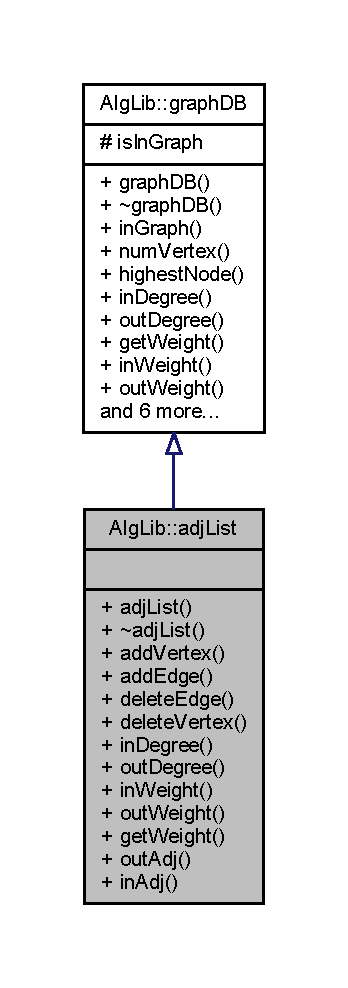
\includegraphics[width=167pt]{class_alg_lib_1_1adj_list__inherit__graph}
\end{center}
\end{figure}


Collaboration diagram for Alg\+Lib\+:\+:adj\+List\+:\nopagebreak
\begin{figure}[H]
\begin{center}
\leavevmode
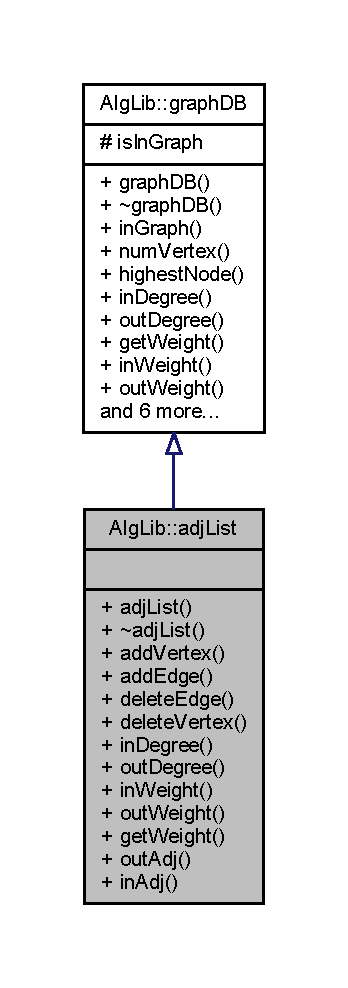
\includegraphics[width=167pt]{class_alg_lib_1_1adj_list__coll__graph}
\end{center}
\end{figure}
\subsection*{Public Member Functions}
\begin{DoxyCompactItemize}
\item 
\hyperlink{class_alg_lib_1_1adj_list_a5e849290c4eb81596d9940d689826099}{adj\+List} (int num\+Vertices=0)
\item 
virtual \hyperlink{class_alg_lib_1_1adj_list_a2dea5320bf4658b69cad9c31e7bf4ae7}{$\sim$adj\+List} ()
\item 
virtual void \hyperlink{class_alg_lib_1_1adj_list_a15380331b1b6b6b510052b5e43f4ba50}{add\+Vertex} () override
\item 
virtual void \hyperlink{class_alg_lib_1_1adj_list_a1010763e586866d884ebb769df8fba52}{add\+Edge} (int nodeS, int nodeE, double weight=1) override
\item 
virtual void \hyperlink{class_alg_lib_1_1adj_list_a11ced2c2ac3cc989e9c23c6e63dc41c5}{delete\+Edge} (int nodeS, int nodeE) override
\item 
virtual void \hyperlink{class_alg_lib_1_1adj_list_a37fa96194420fd556668dc8c4ce5472f}{delete\+Vertex} (int node) override
\item 
virtual int \hyperlink{class_alg_lib_1_1adj_list_a73b55f7e622358e9ac4f2dbd076b393d}{in\+Degree} (int node) const  override
\item 
virtual int \hyperlink{class_alg_lib_1_1adj_list_a3bb70be60dc28fedf1817c76f5b881f2}{out\+Degree} (int node) const  override
\item 
virtual double \hyperlink{class_alg_lib_1_1adj_list_a74fbc3342cdd18cfbd1a3c26982d03a0}{in\+Weight} (int node) const  override
\item 
virtual double \hyperlink{class_alg_lib_1_1adj_list_aeeabf593091f0d068f77d5ed000ab06b}{out\+Weight} (int node) const  override
\item 
virtual double \hyperlink{class_alg_lib_1_1adj_list_a1f365ed028dd4bdce2fc47119f47dde7}{get\+Weight} (int nodeS, int nodeE) const  override
\item 
virtual std\+::vector$<$ std\+::tuple$<$ int, double $>$ $>$ \hyperlink{class_alg_lib_1_1adj_list_a01a7eb08e676f75a339403079e004e00}{out\+Adj} (int node) const  override
\item 
virtual std\+::vector$<$ std\+::tuple$<$ int, double $>$ $>$ \hyperlink{class_alg_lib_1_1adj_list_a2f8f4af6435990aea3b90b3274bf64bf}{in\+Adj} (int node) const  override
\end{DoxyCompactItemize}
\subsection*{Additional Inherited Members}


\subsection{Detailed Description}


Definition at line 10 of file adj\+List.\+h.



\subsection{Constructor \& Destructor Documentation}
\index{Alg\+Lib\+::adj\+List@{Alg\+Lib\+::adj\+List}!adj\+List@{adj\+List}}
\index{adj\+List@{adj\+List}!Alg\+Lib\+::adj\+List@{Alg\+Lib\+::adj\+List}}
\subsubsection[{\texorpdfstring{adj\+List(int num\+Vertices=0)}{adjList(int numVertices=0)}}]{\setlength{\rightskip}{0pt plus 5cm}Alg\+Lib\+::adj\+List\+::adj\+List (
\begin{DoxyParamCaption}
\item[{int}]{num\+Vertices = {\ttfamily 0}}
\end{DoxyParamCaption}
)}\hypertarget{class_alg_lib_1_1adj_list_a5e849290c4eb81596d9940d689826099}{}\label{class_alg_lib_1_1adj_list_a5e849290c4eb81596d9940d689826099}
Default constructor 

Definition at line 10 of file adj\+List.\+cpp.

\index{Alg\+Lib\+::adj\+List@{Alg\+Lib\+::adj\+List}!````~adj\+List@{$\sim$adj\+List}}
\index{````~adj\+List@{$\sim$adj\+List}!Alg\+Lib\+::adj\+List@{Alg\+Lib\+::adj\+List}}
\subsubsection[{\texorpdfstring{$\sim$adj\+List()}{~adjList()}}]{\setlength{\rightskip}{0pt plus 5cm}Alg\+Lib\+::adj\+List\+::$\sim$adj\+List (
\begin{DoxyParamCaption}
{}
\end{DoxyParamCaption}
)\hspace{0.3cm}{\ttfamily [virtual]}}\hypertarget{class_alg_lib_1_1adj_list_a2dea5320bf4658b69cad9c31e7bf4ae7}{}\label{class_alg_lib_1_1adj_list_a2dea5320bf4658b69cad9c31e7bf4ae7}
Default destructor 

Definition at line 21 of file adj\+List.\+cpp.



\subsection{Member Function Documentation}
\index{Alg\+Lib\+::adj\+List@{Alg\+Lib\+::adj\+List}!add\+Edge@{add\+Edge}}
\index{add\+Edge@{add\+Edge}!Alg\+Lib\+::adj\+List@{Alg\+Lib\+::adj\+List}}
\subsubsection[{\texorpdfstring{add\+Edge(int node\+S, int node\+E, double weight=1) override}{addEdge(int nodeS, int nodeE, double weight=1) override}}]{\setlength{\rightskip}{0pt plus 5cm}void Alg\+Lib\+::adj\+List\+::add\+Edge (
\begin{DoxyParamCaption}
\item[{int}]{nodeS, }
\item[{int}]{nodeE, }
\item[{double}]{weight = {\ttfamily 1}}
\end{DoxyParamCaption}
)\hspace{0.3cm}{\ttfamily [override]}, {\ttfamily [virtual]}}\hypertarget{class_alg_lib_1_1adj_list_a1010763e586866d884ebb769df8fba52}{}\label{class_alg_lib_1_1adj_list_a1010763e586866d884ebb769df8fba52}


Implements \hyperlink{class_alg_lib_1_1graph_d_b_aeedc15cdbef55a131d7cf3d91778032e}{Alg\+Lib\+::graph\+DB}.



Definition at line 32 of file adj\+List.\+cpp.

\index{Alg\+Lib\+::adj\+List@{Alg\+Lib\+::adj\+List}!add\+Vertex@{add\+Vertex}}
\index{add\+Vertex@{add\+Vertex}!Alg\+Lib\+::adj\+List@{Alg\+Lib\+::adj\+List}}
\subsubsection[{\texorpdfstring{add\+Vertex() override}{addVertex() override}}]{\setlength{\rightskip}{0pt plus 5cm}void Alg\+Lib\+::adj\+List\+::add\+Vertex (
\begin{DoxyParamCaption}
{}
\end{DoxyParamCaption}
)\hspace{0.3cm}{\ttfamily [override]}, {\ttfamily [virtual]}}\hypertarget{class_alg_lib_1_1adj_list_a15380331b1b6b6b510052b5e43f4ba50}{}\label{class_alg_lib_1_1adj_list_a15380331b1b6b6b510052b5e43f4ba50}


Implements \hyperlink{class_alg_lib_1_1graph_d_b_af21b1c41a94e6240b661bbe76f9fcb35}{Alg\+Lib\+::graph\+DB}.



Definition at line 26 of file adj\+List.\+cpp.

\index{Alg\+Lib\+::adj\+List@{Alg\+Lib\+::adj\+List}!delete\+Edge@{delete\+Edge}}
\index{delete\+Edge@{delete\+Edge}!Alg\+Lib\+::adj\+List@{Alg\+Lib\+::adj\+List}}
\subsubsection[{\texorpdfstring{delete\+Edge(int node\+S, int node\+E) override}{deleteEdge(int nodeS, int nodeE) override}}]{\setlength{\rightskip}{0pt plus 5cm}void Alg\+Lib\+::adj\+List\+::delete\+Edge (
\begin{DoxyParamCaption}
\item[{int}]{nodeS, }
\item[{int}]{nodeE}
\end{DoxyParamCaption}
)\hspace{0.3cm}{\ttfamily [override]}, {\ttfamily [virtual]}}\hypertarget{class_alg_lib_1_1adj_list_a11ced2c2ac3cc989e9c23c6e63dc41c5}{}\label{class_alg_lib_1_1adj_list_a11ced2c2ac3cc989e9c23c6e63dc41c5}


Implements \hyperlink{class_alg_lib_1_1graph_d_b_a01fcc5af770b56fc187e40fb34ec9c9f}{Alg\+Lib\+::graph\+DB}.



Definition at line 55 of file adj\+List.\+cpp.

\index{Alg\+Lib\+::adj\+List@{Alg\+Lib\+::adj\+List}!delete\+Vertex@{delete\+Vertex}}
\index{delete\+Vertex@{delete\+Vertex}!Alg\+Lib\+::adj\+List@{Alg\+Lib\+::adj\+List}}
\subsubsection[{\texorpdfstring{delete\+Vertex(int node) override}{deleteVertex(int node) override}}]{\setlength{\rightskip}{0pt plus 5cm}void Alg\+Lib\+::adj\+List\+::delete\+Vertex (
\begin{DoxyParamCaption}
\item[{int}]{node}
\end{DoxyParamCaption}
)\hspace{0.3cm}{\ttfamily [override]}, {\ttfamily [virtual]}}\hypertarget{class_alg_lib_1_1adj_list_a37fa96194420fd556668dc8c4ce5472f}{}\label{class_alg_lib_1_1adj_list_a37fa96194420fd556668dc8c4ce5472f}


Implements \hyperlink{class_alg_lib_1_1graph_d_b_abb3e87cafce37173f075c27c9c129554}{Alg\+Lib\+::graph\+DB}.



Definition at line 66 of file adj\+List.\+cpp.

\index{Alg\+Lib\+::adj\+List@{Alg\+Lib\+::adj\+List}!get\+Weight@{get\+Weight}}
\index{get\+Weight@{get\+Weight}!Alg\+Lib\+::adj\+List@{Alg\+Lib\+::adj\+List}}
\subsubsection[{\texorpdfstring{get\+Weight(int node\+S, int node\+E) const  override}{getWeight(int nodeS, int nodeE) const  override}}]{\setlength{\rightskip}{0pt plus 5cm}double Alg\+Lib\+::adj\+List\+::get\+Weight (
\begin{DoxyParamCaption}
\item[{int}]{nodeS, }
\item[{int}]{nodeE}
\end{DoxyParamCaption}
) const\hspace{0.3cm}{\ttfamily [override]}, {\ttfamily [virtual]}}\hypertarget{class_alg_lib_1_1adj_list_a1f365ed028dd4bdce2fc47119f47dde7}{}\label{class_alg_lib_1_1adj_list_a1f365ed028dd4bdce2fc47119f47dde7}


Implements \hyperlink{class_alg_lib_1_1graph_d_b_a8b81f180d935d1f80f728c0fef64ca03}{Alg\+Lib\+::graph\+DB}.



Definition at line 155 of file adj\+List.\+cpp.

\index{Alg\+Lib\+::adj\+List@{Alg\+Lib\+::adj\+List}!in\+Adj@{in\+Adj}}
\index{in\+Adj@{in\+Adj}!Alg\+Lib\+::adj\+List@{Alg\+Lib\+::adj\+List}}
\subsubsection[{\texorpdfstring{in\+Adj(int node) const  override}{inAdj(int node) const  override}}]{\setlength{\rightskip}{0pt plus 5cm}std\+::vector$<$ std\+::tuple$<$ int, double $>$ $>$ Alg\+Lib\+::adj\+List\+::in\+Adj (
\begin{DoxyParamCaption}
\item[{int}]{node}
\end{DoxyParamCaption}
) const\hspace{0.3cm}{\ttfamily [override]}, {\ttfamily [virtual]}}\hypertarget{class_alg_lib_1_1adj_list_a2f8f4af6435990aea3b90b3274bf64bf}{}\label{class_alg_lib_1_1adj_list_a2f8f4af6435990aea3b90b3274bf64bf}


Implements \hyperlink{class_alg_lib_1_1graph_d_b_abf67bacae3ae1faa4a9d5260f52ab1ca}{Alg\+Lib\+::graph\+DB}.



Definition at line 139 of file adj\+List.\+cpp.

\index{Alg\+Lib\+::adj\+List@{Alg\+Lib\+::adj\+List}!in\+Degree@{in\+Degree}}
\index{in\+Degree@{in\+Degree}!Alg\+Lib\+::adj\+List@{Alg\+Lib\+::adj\+List}}
\subsubsection[{\texorpdfstring{in\+Degree(int node) const  override}{inDegree(int node) const  override}}]{\setlength{\rightskip}{0pt plus 5cm}int Alg\+Lib\+::adj\+List\+::in\+Degree (
\begin{DoxyParamCaption}
\item[{int}]{node}
\end{DoxyParamCaption}
) const\hspace{0.3cm}{\ttfamily [override]}, {\ttfamily [virtual]}}\hypertarget{class_alg_lib_1_1adj_list_a73b55f7e622358e9ac4f2dbd076b393d}{}\label{class_alg_lib_1_1adj_list_a73b55f7e622358e9ac4f2dbd076b393d}


Implements \hyperlink{class_alg_lib_1_1graph_d_b_a06faf4feb26d18b4491c5671158155f0}{Alg\+Lib\+::graph\+DB}.



Definition at line 85 of file adj\+List.\+cpp.

\index{Alg\+Lib\+::adj\+List@{Alg\+Lib\+::adj\+List}!in\+Weight@{in\+Weight}}
\index{in\+Weight@{in\+Weight}!Alg\+Lib\+::adj\+List@{Alg\+Lib\+::adj\+List}}
\subsubsection[{\texorpdfstring{in\+Weight(int node) const  override}{inWeight(int node) const  override}}]{\setlength{\rightskip}{0pt plus 5cm}double Alg\+Lib\+::adj\+List\+::in\+Weight (
\begin{DoxyParamCaption}
\item[{int}]{node}
\end{DoxyParamCaption}
) const\hspace{0.3cm}{\ttfamily [override]}, {\ttfamily [virtual]}}\hypertarget{class_alg_lib_1_1adj_list_a74fbc3342cdd18cfbd1a3c26982d03a0}{}\label{class_alg_lib_1_1adj_list_a74fbc3342cdd18cfbd1a3c26982d03a0}


Implements \hyperlink{class_alg_lib_1_1graph_d_b_a873a4aa752f53702fad8cd36ab409c0e}{Alg\+Lib\+::graph\+DB}.



Definition at line 110 of file adj\+List.\+cpp.

\index{Alg\+Lib\+::adj\+List@{Alg\+Lib\+::adj\+List}!out\+Adj@{out\+Adj}}
\index{out\+Adj@{out\+Adj}!Alg\+Lib\+::adj\+List@{Alg\+Lib\+::adj\+List}}
\subsubsection[{\texorpdfstring{out\+Adj(int node) const  override}{outAdj(int node) const  override}}]{\setlength{\rightskip}{0pt plus 5cm}std\+::vector$<$ std\+::tuple$<$ int, double $>$ $>$ Alg\+Lib\+::adj\+List\+::out\+Adj (
\begin{DoxyParamCaption}
\item[{int}]{node}
\end{DoxyParamCaption}
) const\hspace{0.3cm}{\ttfamily [override]}, {\ttfamily [virtual]}}\hypertarget{class_alg_lib_1_1adj_list_a01a7eb08e676f75a339403079e004e00}{}\label{class_alg_lib_1_1adj_list_a01a7eb08e676f75a339403079e004e00}


Implements \hyperlink{class_alg_lib_1_1graph_d_b_ae3c91d0775e8c2b28824a11f55571665}{Alg\+Lib\+::graph\+DB}.



Definition at line 134 of file adj\+List.\+cpp.

\index{Alg\+Lib\+::adj\+List@{Alg\+Lib\+::adj\+List}!out\+Degree@{out\+Degree}}
\index{out\+Degree@{out\+Degree}!Alg\+Lib\+::adj\+List@{Alg\+Lib\+::adj\+List}}
\subsubsection[{\texorpdfstring{out\+Degree(int node) const  override}{outDegree(int node) const  override}}]{\setlength{\rightskip}{0pt plus 5cm}int Alg\+Lib\+::adj\+List\+::out\+Degree (
\begin{DoxyParamCaption}
\item[{int}]{node}
\end{DoxyParamCaption}
) const\hspace{0.3cm}{\ttfamily [override]}, {\ttfamily [virtual]}}\hypertarget{class_alg_lib_1_1adj_list_a3bb70be60dc28fedf1817c76f5b881f2}{}\label{class_alg_lib_1_1adj_list_a3bb70be60dc28fedf1817c76f5b881f2}


Implements \hyperlink{class_alg_lib_1_1graph_d_b_a8ac8d9aa118a2584d36d881f2f22a0c8}{Alg\+Lib\+::graph\+DB}.



Definition at line 100 of file adj\+List.\+cpp.

\index{Alg\+Lib\+::adj\+List@{Alg\+Lib\+::adj\+List}!out\+Weight@{out\+Weight}}
\index{out\+Weight@{out\+Weight}!Alg\+Lib\+::adj\+List@{Alg\+Lib\+::adj\+List}}
\subsubsection[{\texorpdfstring{out\+Weight(int node) const  override}{outWeight(int node) const  override}}]{\setlength{\rightskip}{0pt plus 5cm}double Alg\+Lib\+::adj\+List\+::out\+Weight (
\begin{DoxyParamCaption}
\item[{int}]{node}
\end{DoxyParamCaption}
) const\hspace{0.3cm}{\ttfamily [override]}, {\ttfamily [virtual]}}\hypertarget{class_alg_lib_1_1adj_list_aeeabf593091f0d068f77d5ed000ab06b}{}\label{class_alg_lib_1_1adj_list_aeeabf593091f0d068f77d5ed000ab06b}


Implements \hyperlink{class_alg_lib_1_1graph_d_b_a86dea18aed8b3bbcfaf834776d36f20f}{Alg\+Lib\+::graph\+DB}.



Definition at line 126 of file adj\+List.\+cpp.



The documentation for this class was generated from the following files\+:\begin{DoxyCompactItemize}
\item 
D\+:/\+Data/\+Desktop/\+Github/include/\hyperlink{adj_list_8h}{adj\+List.\+h}\item 
D\+:/\+Data/\+Desktop/\+Github/src/\+Graph/\hyperlink{adj_list_8cpp}{adj\+List.\+cpp}\end{DoxyCompactItemize}

\hypertarget{class_alg_lib_1_1adj_matrix}{}\section{Alg\+Lib\+:\+:adj\+Matrix Class Reference}
\label{class_alg_lib_1_1adj_matrix}\index{Alg\+Lib\+::adj\+Matrix@{Alg\+Lib\+::adj\+Matrix}}


{\ttfamily \#include $<$adj\+Matrix.\+h$>$}



Inheritance diagram for Alg\+Lib\+:\+:adj\+Matrix\+:\nopagebreak
\begin{figure}[H]
\begin{center}
\leavevmode
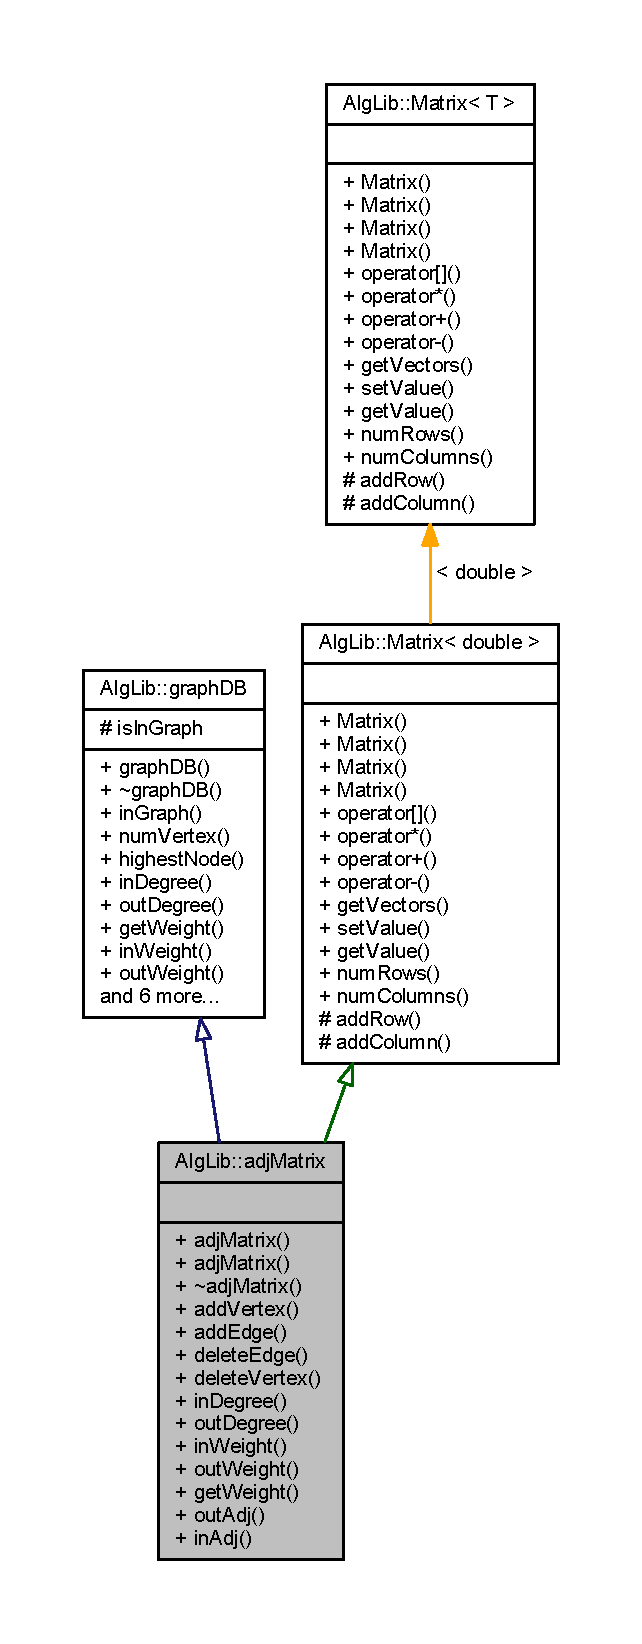
\includegraphics[height=550pt]{class_alg_lib_1_1adj_matrix__inherit__graph}
\end{center}
\end{figure}


Collaboration diagram for Alg\+Lib\+:\+:adj\+Matrix\+:\nopagebreak
\begin{figure}[H]
\begin{center}
\leavevmode
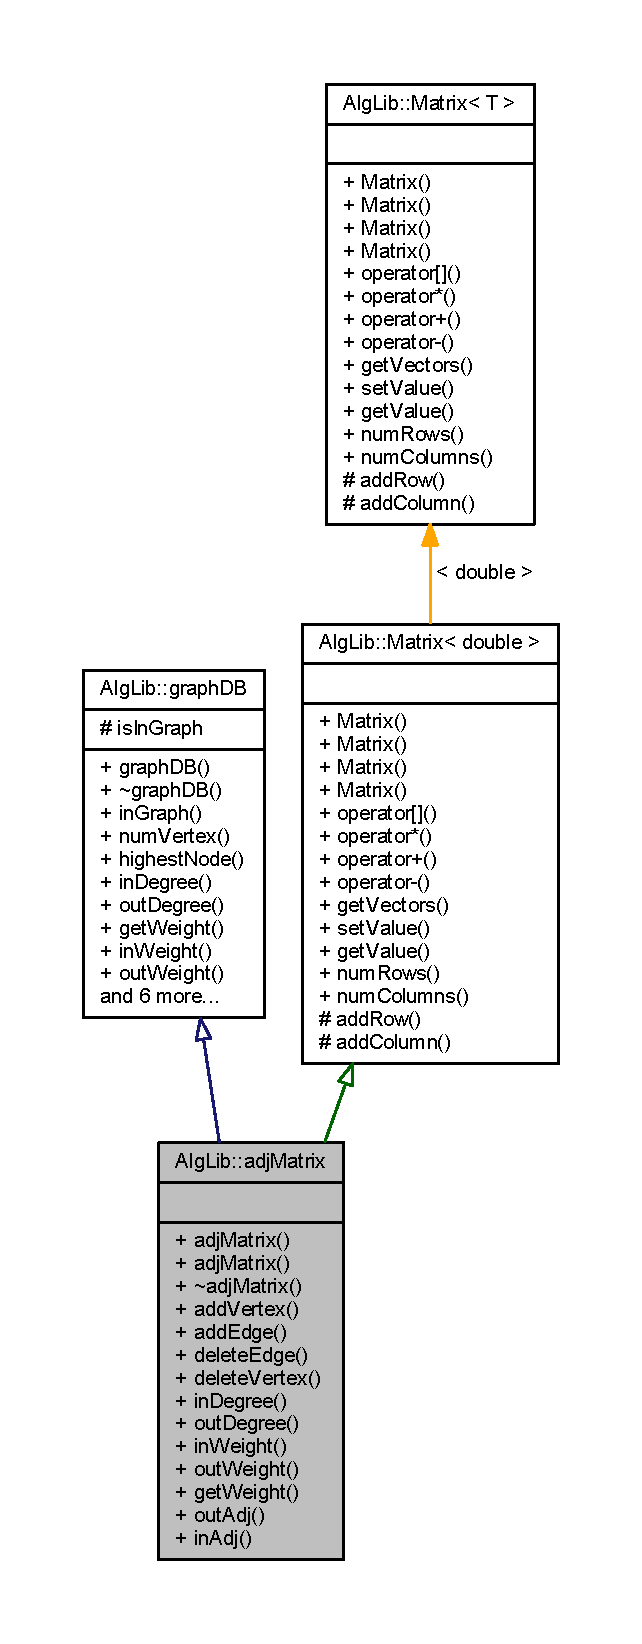
\includegraphics[height=550pt]{class_alg_lib_1_1adj_matrix__coll__graph}
\end{center}
\end{figure}
\subsection*{Public Member Functions}
\begin{DoxyCompactItemize}
\item 
\hyperlink{class_alg_lib_1_1adj_matrix_afed0a27060baa109a23159a5f2685914}{adj\+Matrix} (int num\+Vertices=0)
\begin{DoxyCompactList}\small\item\em (one liner) \end{DoxyCompactList}\item 
\hyperlink{class_alg_lib_1_1adj_matrix_ac612948d3f6ded49591cc7810609a7c2}{adj\+Matrix} (const \hyperlink{class_alg_lib_1_1_matrix}{Matrix}$<$ double $>$ \&other)
\item 
virtual \hyperlink{class_alg_lib_1_1adj_matrix_ae2cdc4fe2471a1358fe0a746a67e8403}{$\sim$adj\+Matrix} ()
\item 
virtual void \hyperlink{class_alg_lib_1_1adj_matrix_a55d736fcb0d25028df7e4775d0b7fa53}{add\+Vertex} () override
\item 
virtual void \hyperlink{class_alg_lib_1_1adj_matrix_a4ca87cc5146e1a1e8967a5cd358711cc}{add\+Edge} (int nodeS, int nodeE, double weight=1) override
\item 
virtual void \hyperlink{class_alg_lib_1_1adj_matrix_ac644ad4932439fea257938c42c7f6ec3}{delete\+Edge} (int nodeS, int nodeE) override
\item 
virtual void \hyperlink{class_alg_lib_1_1adj_matrix_a7e59572f5c9c80853364132cd92eb9a0}{delete\+Vertex} (int node) override
\item 
virtual int \hyperlink{class_alg_lib_1_1adj_matrix_a50039a0fb126b3996b30e3b9fd8e7933}{in\+Degree} (int node) const  override
\item 
virtual int \hyperlink{class_alg_lib_1_1adj_matrix_afbe220e5939f2c5bb621b482904eeef0}{out\+Degree} (int node) const  override
\item 
virtual double \hyperlink{class_alg_lib_1_1adj_matrix_aab4ecb9801ba43d2ce3c0f542e44643e}{in\+Weight} (int node) const  override
\item 
virtual double \hyperlink{class_alg_lib_1_1adj_matrix_a3d807c32353c656f362ed356c4f3d1ed}{out\+Weight} (int node) const  override
\item 
virtual double \hyperlink{class_alg_lib_1_1adj_matrix_a05bbb7b2b30f83c6b89ff75dc6cc84ea}{get\+Weight} (int nodeS, int nodeE) const  override
\item 
virtual std\+::vector$<$ std\+::tuple$<$ int, double $>$ $>$ \hyperlink{class_alg_lib_1_1adj_matrix_a0e8e97ad4fba9e2862d36ab1be2324f1}{out\+Adj} (int node) const  override
\item 
virtual std\+::vector$<$ std\+::tuple$<$ int, double $>$ $>$ \hyperlink{class_alg_lib_1_1adj_matrix_a52a5e7ac8fdd3bf11aa6dcf38d800ecb}{in\+Adj} (int node) const  override
\end{DoxyCompactItemize}
\subsection*{Additional Inherited Members}


\subsection{Detailed Description}


Definition at line 10 of file adj\+Matrix.\+h.



\subsection{Constructor \& Destructor Documentation}
\index{Alg\+Lib\+::adj\+Matrix@{Alg\+Lib\+::adj\+Matrix}!adj\+Matrix@{adj\+Matrix}}
\index{adj\+Matrix@{adj\+Matrix}!Alg\+Lib\+::adj\+Matrix@{Alg\+Lib\+::adj\+Matrix}}
\subsubsection[{\texorpdfstring{adj\+Matrix(int num\+Vertices=0)}{adjMatrix(int numVertices=0)}}]{\setlength{\rightskip}{0pt plus 5cm}Alg\+Lib\+::adj\+Matrix\+::adj\+Matrix (
\begin{DoxyParamCaption}
\item[{int}]{num\+Vertices = {\ttfamily 0}}
\end{DoxyParamCaption}
)}\hypertarget{class_alg_lib_1_1adj_matrix_afed0a27060baa109a23159a5f2685914}{}\label{class_alg_lib_1_1adj_matrix_afed0a27060baa109a23159a5f2685914}


(one liner) 

Default constructor

(documentation goes here) 

Definition at line 12 of file adj\+Matrix.\+cpp.

\index{Alg\+Lib\+::adj\+Matrix@{Alg\+Lib\+::adj\+Matrix}!adj\+Matrix@{adj\+Matrix}}
\index{adj\+Matrix@{adj\+Matrix}!Alg\+Lib\+::adj\+Matrix@{Alg\+Lib\+::adj\+Matrix}}
\subsubsection[{\texorpdfstring{adj\+Matrix(const Matrix$<$ double $>$ \&other)}{adjMatrix(const Matrix< double > &other)}}]{\setlength{\rightskip}{0pt plus 5cm}Alg\+Lib\+::adj\+Matrix\+::adj\+Matrix (
\begin{DoxyParamCaption}
\item[{const {\bf Matrix}$<$ double $>$ \&}]{other}
\end{DoxyParamCaption}
)}\hypertarget{class_alg_lib_1_1adj_matrix_ac612948d3f6ded49591cc7810609a7c2}{}\label{class_alg_lib_1_1adj_matrix_ac612948d3f6ded49591cc7810609a7c2}


Definition at line 19 of file adj\+Matrix.\+cpp.

\index{Alg\+Lib\+::adj\+Matrix@{Alg\+Lib\+::adj\+Matrix}!````~adj\+Matrix@{$\sim$adj\+Matrix}}
\index{````~adj\+Matrix@{$\sim$adj\+Matrix}!Alg\+Lib\+::adj\+Matrix@{Alg\+Lib\+::adj\+Matrix}}
\subsubsection[{\texorpdfstring{$\sim$adj\+Matrix()}{~adjMatrix()}}]{\setlength{\rightskip}{0pt plus 5cm}Alg\+Lib\+::adj\+Matrix\+::$\sim$adj\+Matrix (
\begin{DoxyParamCaption}
{}
\end{DoxyParamCaption}
)\hspace{0.3cm}{\ttfamily [virtual]}}\hypertarget{class_alg_lib_1_1adj_matrix_ae2cdc4fe2471a1358fe0a746a67e8403}{}\label{class_alg_lib_1_1adj_matrix_ae2cdc4fe2471a1358fe0a746a67e8403}
Default destructor 

Definition at line 26 of file adj\+Matrix.\+cpp.



\subsection{Member Function Documentation}
\index{Alg\+Lib\+::adj\+Matrix@{Alg\+Lib\+::adj\+Matrix}!add\+Edge@{add\+Edge}}
\index{add\+Edge@{add\+Edge}!Alg\+Lib\+::adj\+Matrix@{Alg\+Lib\+::adj\+Matrix}}
\subsubsection[{\texorpdfstring{add\+Edge(int node\+S, int node\+E, double weight=1) override}{addEdge(int nodeS, int nodeE, double weight=1) override}}]{\setlength{\rightskip}{0pt plus 5cm}void Alg\+Lib\+::adj\+Matrix\+::add\+Edge (
\begin{DoxyParamCaption}
\item[{int}]{nodeS, }
\item[{int}]{nodeE, }
\item[{double}]{weight = {\ttfamily 1}}
\end{DoxyParamCaption}
)\hspace{0.3cm}{\ttfamily [override]}, {\ttfamily [virtual]}}\hypertarget{class_alg_lib_1_1adj_matrix_a4ca87cc5146e1a1e8967a5cd358711cc}{}\label{class_alg_lib_1_1adj_matrix_a4ca87cc5146e1a1e8967a5cd358711cc}


Implements \hyperlink{class_alg_lib_1_1graph_d_b_aeedc15cdbef55a131d7cf3d91778032e}{Alg\+Lib\+::graph\+DB}.



Definition at line 38 of file adj\+Matrix.\+cpp.

\index{Alg\+Lib\+::adj\+Matrix@{Alg\+Lib\+::adj\+Matrix}!add\+Vertex@{add\+Vertex}}
\index{add\+Vertex@{add\+Vertex}!Alg\+Lib\+::adj\+Matrix@{Alg\+Lib\+::adj\+Matrix}}
\subsubsection[{\texorpdfstring{add\+Vertex() override}{addVertex() override}}]{\setlength{\rightskip}{0pt plus 5cm}void Alg\+Lib\+::adj\+Matrix\+::add\+Vertex (
\begin{DoxyParamCaption}
{}
\end{DoxyParamCaption}
)\hspace{0.3cm}{\ttfamily [override]}, {\ttfamily [virtual]}}\hypertarget{class_alg_lib_1_1adj_matrix_a55d736fcb0d25028df7e4775d0b7fa53}{}\label{class_alg_lib_1_1adj_matrix_a55d736fcb0d25028df7e4775d0b7fa53}


Implements \hyperlink{class_alg_lib_1_1graph_d_b_af21b1c41a94e6240b661bbe76f9fcb35}{Alg\+Lib\+::graph\+DB}.



Definition at line 31 of file adj\+Matrix.\+cpp.

\index{Alg\+Lib\+::adj\+Matrix@{Alg\+Lib\+::adj\+Matrix}!delete\+Edge@{delete\+Edge}}
\index{delete\+Edge@{delete\+Edge}!Alg\+Lib\+::adj\+Matrix@{Alg\+Lib\+::adj\+Matrix}}
\subsubsection[{\texorpdfstring{delete\+Edge(int node\+S, int node\+E) override}{deleteEdge(int nodeS, int nodeE) override}}]{\setlength{\rightskip}{0pt plus 5cm}void Alg\+Lib\+::adj\+Matrix\+::delete\+Edge (
\begin{DoxyParamCaption}
\item[{int}]{nodeS, }
\item[{int}]{nodeE}
\end{DoxyParamCaption}
)\hspace{0.3cm}{\ttfamily [override]}, {\ttfamily [virtual]}}\hypertarget{class_alg_lib_1_1adj_matrix_ac644ad4932439fea257938c42c7f6ec3}{}\label{class_alg_lib_1_1adj_matrix_ac644ad4932439fea257938c42c7f6ec3}


Implements \hyperlink{class_alg_lib_1_1graph_d_b_a01fcc5af770b56fc187e40fb34ec9c9f}{Alg\+Lib\+::graph\+DB}.



Definition at line 43 of file adj\+Matrix.\+cpp.

\index{Alg\+Lib\+::adj\+Matrix@{Alg\+Lib\+::adj\+Matrix}!delete\+Vertex@{delete\+Vertex}}
\index{delete\+Vertex@{delete\+Vertex}!Alg\+Lib\+::adj\+Matrix@{Alg\+Lib\+::adj\+Matrix}}
\subsubsection[{\texorpdfstring{delete\+Vertex(int node) override}{deleteVertex(int node) override}}]{\setlength{\rightskip}{0pt plus 5cm}void Alg\+Lib\+::adj\+Matrix\+::delete\+Vertex (
\begin{DoxyParamCaption}
\item[{int}]{node}
\end{DoxyParamCaption}
)\hspace{0.3cm}{\ttfamily [override]}, {\ttfamily [virtual]}}\hypertarget{class_alg_lib_1_1adj_matrix_a7e59572f5c9c80853364132cd92eb9a0}{}\label{class_alg_lib_1_1adj_matrix_a7e59572f5c9c80853364132cd92eb9a0}


Implements \hyperlink{class_alg_lib_1_1graph_d_b_abb3e87cafce37173f075c27c9c129554}{Alg\+Lib\+::graph\+DB}.



Definition at line 48 of file adj\+Matrix.\+cpp.

\index{Alg\+Lib\+::adj\+Matrix@{Alg\+Lib\+::adj\+Matrix}!get\+Weight@{get\+Weight}}
\index{get\+Weight@{get\+Weight}!Alg\+Lib\+::adj\+Matrix@{Alg\+Lib\+::adj\+Matrix}}
\subsubsection[{\texorpdfstring{get\+Weight(int node\+S, int node\+E) const  override}{getWeight(int nodeS, int nodeE) const  override}}]{\setlength{\rightskip}{0pt plus 5cm}double Alg\+Lib\+::adj\+Matrix\+::get\+Weight (
\begin{DoxyParamCaption}
\item[{int}]{nodeS, }
\item[{int}]{nodeE}
\end{DoxyParamCaption}
) const\hspace{0.3cm}{\ttfamily [override]}, {\ttfamily [virtual]}}\hypertarget{class_alg_lib_1_1adj_matrix_a05bbb7b2b30f83c6b89ff75dc6cc84ea}{}\label{class_alg_lib_1_1adj_matrix_a05bbb7b2b30f83c6b89ff75dc6cc84ea}


Implements \hyperlink{class_alg_lib_1_1graph_d_b_a8b81f180d935d1f80f728c0fef64ca03}{Alg\+Lib\+::graph\+DB}.



Definition at line 130 of file adj\+Matrix.\+cpp.

\index{Alg\+Lib\+::adj\+Matrix@{Alg\+Lib\+::adj\+Matrix}!in\+Adj@{in\+Adj}}
\index{in\+Adj@{in\+Adj}!Alg\+Lib\+::adj\+Matrix@{Alg\+Lib\+::adj\+Matrix}}
\subsubsection[{\texorpdfstring{in\+Adj(int node) const  override}{inAdj(int node) const  override}}]{\setlength{\rightskip}{0pt plus 5cm}std\+::vector$<$ std\+::tuple$<$ int, double $>$ $>$ Alg\+Lib\+::adj\+Matrix\+::in\+Adj (
\begin{DoxyParamCaption}
\item[{int}]{node}
\end{DoxyParamCaption}
) const\hspace{0.3cm}{\ttfamily [override]}, {\ttfamily [virtual]}}\hypertarget{class_alg_lib_1_1adj_matrix_a52a5e7ac8fdd3bf11aa6dcf38d800ecb}{}\label{class_alg_lib_1_1adj_matrix_a52a5e7ac8fdd3bf11aa6dcf38d800ecb}


Implements \hyperlink{class_alg_lib_1_1graph_d_b_abf67bacae3ae1faa4a9d5260f52ab1ca}{Alg\+Lib\+::graph\+DB}.



Definition at line 116 of file adj\+Matrix.\+cpp.

\index{Alg\+Lib\+::adj\+Matrix@{Alg\+Lib\+::adj\+Matrix}!in\+Degree@{in\+Degree}}
\index{in\+Degree@{in\+Degree}!Alg\+Lib\+::adj\+Matrix@{Alg\+Lib\+::adj\+Matrix}}
\subsubsection[{\texorpdfstring{in\+Degree(int node) const  override}{inDegree(int node) const  override}}]{\setlength{\rightskip}{0pt plus 5cm}int Alg\+Lib\+::adj\+Matrix\+::in\+Degree (
\begin{DoxyParamCaption}
\item[{int}]{node}
\end{DoxyParamCaption}
) const\hspace{0.3cm}{\ttfamily [override]}, {\ttfamily [virtual]}}\hypertarget{class_alg_lib_1_1adj_matrix_a50039a0fb126b3996b30e3b9fd8e7933}{}\label{class_alg_lib_1_1adj_matrix_a50039a0fb126b3996b30e3b9fd8e7933}


Implements \hyperlink{class_alg_lib_1_1graph_d_b_a06faf4feb26d18b4491c5671158155f0}{Alg\+Lib\+::graph\+DB}.



Definition at line 61 of file adj\+Matrix.\+cpp.

\index{Alg\+Lib\+::adj\+Matrix@{Alg\+Lib\+::adj\+Matrix}!in\+Weight@{in\+Weight}}
\index{in\+Weight@{in\+Weight}!Alg\+Lib\+::adj\+Matrix@{Alg\+Lib\+::adj\+Matrix}}
\subsubsection[{\texorpdfstring{in\+Weight(int node) const  override}{inWeight(int node) const  override}}]{\setlength{\rightskip}{0pt plus 5cm}double Alg\+Lib\+::adj\+Matrix\+::in\+Weight (
\begin{DoxyParamCaption}
\item[{int}]{node}
\end{DoxyParamCaption}
) const\hspace{0.3cm}{\ttfamily [override]}, {\ttfamily [virtual]}}\hypertarget{class_alg_lib_1_1adj_matrix_aab4ecb9801ba43d2ce3c0f542e44643e}{}\label{class_alg_lib_1_1adj_matrix_aab4ecb9801ba43d2ce3c0f542e44643e}


Implements \hyperlink{class_alg_lib_1_1graph_d_b_a873a4aa752f53702fad8cd36ab409c0e}{Alg\+Lib\+::graph\+DB}.



Definition at line 83 of file adj\+Matrix.\+cpp.

\index{Alg\+Lib\+::adj\+Matrix@{Alg\+Lib\+::adj\+Matrix}!out\+Adj@{out\+Adj}}
\index{out\+Adj@{out\+Adj}!Alg\+Lib\+::adj\+Matrix@{Alg\+Lib\+::adj\+Matrix}}
\subsubsection[{\texorpdfstring{out\+Adj(int node) const  override}{outAdj(int node) const  override}}]{\setlength{\rightskip}{0pt plus 5cm}std\+::vector$<$ std\+::tuple$<$ int, double $>$ $>$ Alg\+Lib\+::adj\+Matrix\+::out\+Adj (
\begin{DoxyParamCaption}
\item[{int}]{node}
\end{DoxyParamCaption}
) const\hspace{0.3cm}{\ttfamily [override]}, {\ttfamily [virtual]}}\hypertarget{class_alg_lib_1_1adj_matrix_a0e8e97ad4fba9e2862d36ab1be2324f1}{}\label{class_alg_lib_1_1adj_matrix_a0e8e97ad4fba9e2862d36ab1be2324f1}


Implements \hyperlink{class_alg_lib_1_1graph_d_b_ae3c91d0775e8c2b28824a11f55571665}{Alg\+Lib\+::graph\+DB}.



Definition at line 103 of file adj\+Matrix.\+cpp.

\index{Alg\+Lib\+::adj\+Matrix@{Alg\+Lib\+::adj\+Matrix}!out\+Degree@{out\+Degree}}
\index{out\+Degree@{out\+Degree}!Alg\+Lib\+::adj\+Matrix@{Alg\+Lib\+::adj\+Matrix}}
\subsubsection[{\texorpdfstring{out\+Degree(int node) const  override}{outDegree(int node) const  override}}]{\setlength{\rightskip}{0pt plus 5cm}int Alg\+Lib\+::adj\+Matrix\+::out\+Degree (
\begin{DoxyParamCaption}
\item[{int}]{node}
\end{DoxyParamCaption}
) const\hspace{0.3cm}{\ttfamily [override]}, {\ttfamily [virtual]}}\hypertarget{class_alg_lib_1_1adj_matrix_afbe220e5939f2c5bb621b482904eeef0}{}\label{class_alg_lib_1_1adj_matrix_afbe220e5939f2c5bb621b482904eeef0}


Implements \hyperlink{class_alg_lib_1_1graph_d_b_a8ac8d9aa118a2584d36d881f2f22a0c8}{Alg\+Lib\+::graph\+DB}.



Definition at line 72 of file adj\+Matrix.\+cpp.

\index{Alg\+Lib\+::adj\+Matrix@{Alg\+Lib\+::adj\+Matrix}!out\+Weight@{out\+Weight}}
\index{out\+Weight@{out\+Weight}!Alg\+Lib\+::adj\+Matrix@{Alg\+Lib\+::adj\+Matrix}}
\subsubsection[{\texorpdfstring{out\+Weight(int node) const  override}{outWeight(int node) const  override}}]{\setlength{\rightskip}{0pt plus 5cm}double Alg\+Lib\+::adj\+Matrix\+::out\+Weight (
\begin{DoxyParamCaption}
\item[{int}]{node}
\end{DoxyParamCaption}
) const\hspace{0.3cm}{\ttfamily [override]}, {\ttfamily [virtual]}}\hypertarget{class_alg_lib_1_1adj_matrix_a3d807c32353c656f362ed356c4f3d1ed}{}\label{class_alg_lib_1_1adj_matrix_a3d807c32353c656f362ed356c4f3d1ed}


Implements \hyperlink{class_alg_lib_1_1graph_d_b_a86dea18aed8b3bbcfaf834776d36f20f}{Alg\+Lib\+::graph\+DB}.



Definition at line 93 of file adj\+Matrix.\+cpp.



The documentation for this class was generated from the following files\+:\begin{DoxyCompactItemize}
\item 
D\+:/\+Data/\+Desktop/\+Github/include/\hyperlink{adj_matrix_8h}{adj\+Matrix.\+h}\item 
D\+:/\+Data/\+Desktop/\+Github/src/\+Graph/\hyperlink{adj_matrix_8cpp}{adj\+Matrix.\+cpp}\end{DoxyCompactItemize}

\hypertarget{class_alg_lib_1_1_fraction}{}\section{Alg\+Lib\+:\+:Fraction Class Reference}
\label{class_alg_lib_1_1_fraction}\index{Alg\+Lib\+::\+Fraction@{Alg\+Lib\+::\+Fraction}}


{\ttfamily \#include $<$Fraction.\+h$>$}



Collaboration diagram for Alg\+Lib\+:\+:Fraction\+:\nopagebreak
\begin{figure}[H]
\begin{center}
\leavevmode
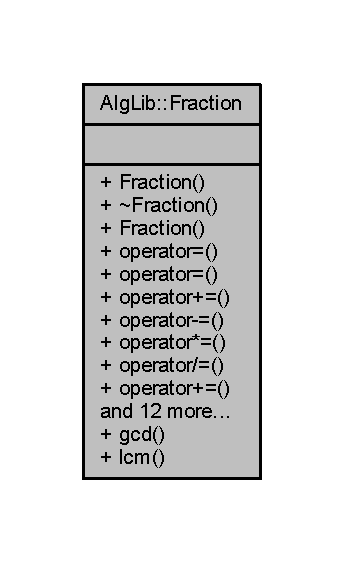
\includegraphics[width=165pt]{class_alg_lib_1_1_fraction__coll__graph}
\end{center}
\end{figure}
\subsection*{Public Member Functions}
\begin{DoxyCompactItemize}
\item 
\hyperlink{class_alg_lib_1_1_fraction_a4f4d5c1e3e177705af049ae1fc4ffb09}{Fraction} ()
\item 
virtual \hyperlink{class_alg_lib_1_1_fraction_aed844397d914c8b54fc5f8dd1893ea63}{$\sim$\+Fraction} ()
\item 
\hyperlink{class_alg_lib_1_1_fraction_a7d979fdca2756edb38e2f6e02c456945}{Fraction} (const \hyperlink{class_alg_lib_1_1_fraction}{Fraction} \&other)
\item 
virtual \hyperlink{class_alg_lib_1_1_fraction}{Fraction} \& \hyperlink{class_alg_lib_1_1_fraction_a93407b0ce7ebfd38f07a25e476243e46}{operator=} (const \hyperlink{class_alg_lib_1_1_fraction}{Fraction} \&other)
\item 
virtual \hyperlink{class_alg_lib_1_1_fraction}{Fraction} \& \hyperlink{class_alg_lib_1_1_fraction_a77f3cf204458ae50677be0a3d2fca383}{operator=} (const int n)
\item 
virtual \hyperlink{class_alg_lib_1_1_fraction}{Fraction} \& \hyperlink{class_alg_lib_1_1_fraction_afd8e8608c4789bfe09f957e377010275}{operator+=} (const int other)
\item 
virtual \hyperlink{class_alg_lib_1_1_fraction}{Fraction} \& \hyperlink{class_alg_lib_1_1_fraction_aa54117f58580597ec4159769c25745b0}{operator-\/=} (const int other)
\item 
virtual \hyperlink{class_alg_lib_1_1_fraction}{Fraction} \& \hyperlink{class_alg_lib_1_1_fraction_a2fcea0923ebd05d7e5fcbba499734da3}{operator$\ast$=} (const int other)
\item 
virtual \hyperlink{class_alg_lib_1_1_fraction}{Fraction} \& \hyperlink{class_alg_lib_1_1_fraction_ad844a41ab7d8a4155e8a563d70fca706}{operator/=} (const int other)
\item 
virtual \hyperlink{class_alg_lib_1_1_fraction}{Fraction} \& \hyperlink{class_alg_lib_1_1_fraction_ae91d89df1b4a0992fa23316a1736131a}{operator+=} (const \hyperlink{class_alg_lib_1_1_fraction}{Fraction} \&other)
\item 
virtual \hyperlink{class_alg_lib_1_1_fraction}{Fraction} \& \hyperlink{class_alg_lib_1_1_fraction_a5e99fb29b42a5e4c7f042b20c89787f4}{operator-\/=} (const \hyperlink{class_alg_lib_1_1_fraction}{Fraction} \&other)
\item 
virtual \hyperlink{class_alg_lib_1_1_fraction}{Fraction} \& \hyperlink{class_alg_lib_1_1_fraction_a43503b8b709459edb0445eceeb0eea55}{operator$\ast$=} (const \hyperlink{class_alg_lib_1_1_fraction}{Fraction} \&other)
\item 
virtual \hyperlink{class_alg_lib_1_1_fraction}{Fraction} \& \hyperlink{class_alg_lib_1_1_fraction_a5e0a2558eb0566f86826c8c97275b391}{operator/=} (const \hyperlink{class_alg_lib_1_1_fraction}{Fraction} \&other)
\item 
virtual bool \hyperlink{class_alg_lib_1_1_fraction_aa6d4323da2799ffda77543d955ef0ae7}{operator$>$} (const \hyperlink{class_alg_lib_1_1_fraction}{Fraction} \&other)
\item 
virtual bool \hyperlink{class_alg_lib_1_1_fraction_aad1c9b3fec500e7538435d4e3e329101}{operator$<$} (const \hyperlink{class_alg_lib_1_1_fraction}{Fraction} \&other)
\item 
virtual bool \hyperlink{class_alg_lib_1_1_fraction_a5f61edd6dbf3616996fa44195701fc00}{operator==} (const \hyperlink{class_alg_lib_1_1_fraction}{Fraction} \&other)
\item 
virtual bool \hyperlink{class_alg_lib_1_1_fraction_a1e3623fabfa02de42052943a319fc2b5}{operator!=} (const \hyperlink{class_alg_lib_1_1_fraction}{Fraction} \&other)
\item 
virtual bool \hyperlink{class_alg_lib_1_1_fraction_ac13e475bba27f25e1b1f8b2de3aed36c}{operator$>$=} (const \hyperlink{class_alg_lib_1_1_fraction}{Fraction} \&other)
\item 
virtual bool \hyperlink{class_alg_lib_1_1_fraction_a13e7582666ef2218c3f430302464f4ac}{operator$<$=} (const \hyperlink{class_alg_lib_1_1_fraction}{Fraction} \&other)
\item 
\hyperlink{class_alg_lib_1_1_fraction_a6d2b59a227bfcb55e852f07751949ff4}{Fraction} (int n, int d=1)
\begin{DoxyCompactList}\small\item\em (one liner) \end{DoxyCompactList}\item 
virtual std\+::string \hyperlink{class_alg_lib_1_1_fraction_a28d61a593ab5abaac86f091398cf7e00}{to\+String} ()
\item 
virtual double \hyperlink{class_alg_lib_1_1_fraction_af56bf89da08dd47e3dfc28d365195d46}{get\+Value} () const 
\end{DoxyCompactItemize}
\subsection*{Static Public Member Functions}
\begin{DoxyCompactItemize}
\item 
static int \hyperlink{class_alg_lib_1_1_fraction_ab63e88e7785efe993305ff803e35efa2}{gcd} (int a, int b)
\item 
static int \hyperlink{class_alg_lib_1_1_fraction_a6f95fe4660cfda996102bf5f4240fe4c}{lcm} (int a, int b)
\end{DoxyCompactItemize}
\subsection*{Friends}
\begin{DoxyCompactItemize}
\item 
\hyperlink{class_alg_lib_1_1_fraction}{Fraction} \hyperlink{class_alg_lib_1_1_fraction_a225c4aec1a9cdd366b04be2642ecf3bc}{operator+} (const \hyperlink{class_alg_lib_1_1_fraction}{Fraction} \&f1, const \hyperlink{class_alg_lib_1_1_fraction}{Fraction} \&f2)
\item 
\hyperlink{class_alg_lib_1_1_fraction}{Fraction} \hyperlink{class_alg_lib_1_1_fraction_aa93e0ab89fa477f3b044cf5826df7c14}{operator-\/} (const \hyperlink{class_alg_lib_1_1_fraction}{Fraction} \&f1, const \hyperlink{class_alg_lib_1_1_fraction}{Fraction} \&f2)
\item 
\hyperlink{class_alg_lib_1_1_fraction}{Fraction} \hyperlink{class_alg_lib_1_1_fraction_ad106ee756801021779f14e992439db4a}{operator$\ast$} (const \hyperlink{class_alg_lib_1_1_fraction}{Fraction} \&f1, const \hyperlink{class_alg_lib_1_1_fraction}{Fraction} \&f2)
\item 
\hyperlink{class_alg_lib_1_1_fraction}{Fraction} \hyperlink{class_alg_lib_1_1_fraction_a2a185031bd64d6b227509aeacf3b5c69}{operator/} (const \hyperlink{class_alg_lib_1_1_fraction}{Fraction} \&f1, const \hyperlink{class_alg_lib_1_1_fraction}{Fraction} \&f2)
\end{DoxyCompactItemize}


\subsection{Detailed Description}


Definition at line 6 of file Fraction.\+h.



\subsection{Constructor \& Destructor Documentation}
\index{Alg\+Lib\+::\+Fraction@{Alg\+Lib\+::\+Fraction}!Fraction@{Fraction}}
\index{Fraction@{Fraction}!Alg\+Lib\+::\+Fraction@{Alg\+Lib\+::\+Fraction}}
\subsubsection[{\texorpdfstring{Fraction()}{Fraction()}}]{\setlength{\rightskip}{0pt plus 5cm}Alg\+Lib\+::\+Fraction\+::\+Fraction (
\begin{DoxyParamCaption}
{}
\end{DoxyParamCaption}
)}\hypertarget{class_alg_lib_1_1_fraction_a4f4d5c1e3e177705af049ae1fc4ffb09}{}\label{class_alg_lib_1_1_fraction_a4f4d5c1e3e177705af049ae1fc4ffb09}
Default constructor 

Definition at line 59 of file Fraction.\+cpp.

\index{Alg\+Lib\+::\+Fraction@{Alg\+Lib\+::\+Fraction}!````~Fraction@{$\sim$\+Fraction}}
\index{````~Fraction@{$\sim$\+Fraction}!Alg\+Lib\+::\+Fraction@{Alg\+Lib\+::\+Fraction}}
\subsubsection[{\texorpdfstring{$\sim$\+Fraction()}{~Fraction()}}]{\setlength{\rightskip}{0pt plus 5cm}Alg\+Lib\+::\+Fraction\+::$\sim$\+Fraction (
\begin{DoxyParamCaption}
{}
\end{DoxyParamCaption}
)\hspace{0.3cm}{\ttfamily [virtual]}}\hypertarget{class_alg_lib_1_1_fraction_aed844397d914c8b54fc5f8dd1893ea63}{}\label{class_alg_lib_1_1_fraction_aed844397d914c8b54fc5f8dd1893ea63}
Default destructor 

Definition at line 66 of file Fraction.\+cpp.

\index{Alg\+Lib\+::\+Fraction@{Alg\+Lib\+::\+Fraction}!Fraction@{Fraction}}
\index{Fraction@{Fraction}!Alg\+Lib\+::\+Fraction@{Alg\+Lib\+::\+Fraction}}
\subsubsection[{\texorpdfstring{Fraction(const Fraction \&other)}{Fraction(const Fraction &other)}}]{\setlength{\rightskip}{0pt plus 5cm}Alg\+Lib\+::\+Fraction\+::\+Fraction (
\begin{DoxyParamCaption}
\item[{const {\bf Fraction} \&}]{other}
\end{DoxyParamCaption}
)}\hypertarget{class_alg_lib_1_1_fraction_a7d979fdca2756edb38e2f6e02c456945}{}\label{class_alg_lib_1_1_fraction_a7d979fdca2756edb38e2f6e02c456945}
Copy constructor 
\begin{DoxyParams}{Parameters}
{\em other} & Object to copy from \\
\hline
\end{DoxyParams}


Definition at line 71 of file Fraction.\+cpp.

\index{Alg\+Lib\+::\+Fraction@{Alg\+Lib\+::\+Fraction}!Fraction@{Fraction}}
\index{Fraction@{Fraction}!Alg\+Lib\+::\+Fraction@{Alg\+Lib\+::\+Fraction}}
\subsubsection[{\texorpdfstring{Fraction(int n, int d=1)}{Fraction(int n, int d=1)}}]{\setlength{\rightskip}{0pt plus 5cm}Alg\+Lib\+::\+Fraction\+::\+Fraction (
\begin{DoxyParamCaption}
\item[{int}]{n, }
\item[{int}]{d = {\ttfamily 1}}
\end{DoxyParamCaption}
)}\hypertarget{class_alg_lib_1_1_fraction_a6d2b59a227bfcb55e852f07751949ff4}{}\label{class_alg_lib_1_1_fraction_a6d2b59a227bfcb55e852f07751949ff4}


(one liner) 

(documentation goes here) 

Definition at line 149 of file Fraction.\+cpp.



\subsection{Member Function Documentation}
\index{Alg\+Lib\+::\+Fraction@{Alg\+Lib\+::\+Fraction}!gcd@{gcd}}
\index{gcd@{gcd}!Alg\+Lib\+::\+Fraction@{Alg\+Lib\+::\+Fraction}}
\subsubsection[{\texorpdfstring{gcd(int a, int b)}{gcd(int a, int b)}}]{\setlength{\rightskip}{0pt plus 5cm}int Alg\+Lib\+::\+Fraction\+::gcd (
\begin{DoxyParamCaption}
\item[{int}]{a, }
\item[{int}]{b}
\end{DoxyParamCaption}
)\hspace{0.3cm}{\ttfamily [static]}}\hypertarget{class_alg_lib_1_1_fraction_ab63e88e7785efe993305ff803e35efa2}{}\label{class_alg_lib_1_1_fraction_ab63e88e7785efe993305ff803e35efa2}


Definition at line 156 of file Fraction.\+cpp.

\index{Alg\+Lib\+::\+Fraction@{Alg\+Lib\+::\+Fraction}!get\+Value@{get\+Value}}
\index{get\+Value@{get\+Value}!Alg\+Lib\+::\+Fraction@{Alg\+Lib\+::\+Fraction}}
\subsubsection[{\texorpdfstring{get\+Value() const }{getValue() const }}]{\setlength{\rightskip}{0pt plus 5cm}double Alg\+Lib\+::\+Fraction\+::get\+Value (
\begin{DoxyParamCaption}
{}
\end{DoxyParamCaption}
) const\hspace{0.3cm}{\ttfamily [virtual]}}\hypertarget{class_alg_lib_1_1_fraction_af56bf89da08dd47e3dfc28d365195d46}{}\label{class_alg_lib_1_1_fraction_af56bf89da08dd47e3dfc28d365195d46}


Definition at line 21 of file Fraction.\+cpp.

\index{Alg\+Lib\+::\+Fraction@{Alg\+Lib\+::\+Fraction}!lcm@{lcm}}
\index{lcm@{lcm}!Alg\+Lib\+::\+Fraction@{Alg\+Lib\+::\+Fraction}}
\subsubsection[{\texorpdfstring{lcm(int a, int b)}{lcm(int a, int b)}}]{\setlength{\rightskip}{0pt plus 5cm}int Alg\+Lib\+::\+Fraction\+::lcm (
\begin{DoxyParamCaption}
\item[{int}]{a, }
\item[{int}]{b}
\end{DoxyParamCaption}
)\hspace{0.3cm}{\ttfamily [static]}}\hypertarget{class_alg_lib_1_1_fraction_a6f95fe4660cfda996102bf5f4240fe4c}{}\label{class_alg_lib_1_1_fraction_a6f95fe4660cfda996102bf5f4240fe4c}


Definition at line 180 of file Fraction.\+cpp.

\index{Alg\+Lib\+::\+Fraction@{Alg\+Lib\+::\+Fraction}!operator"!=@{operator"!=}}
\index{operator"!=@{operator"!=}!Alg\+Lib\+::\+Fraction@{Alg\+Lib\+::\+Fraction}}
\subsubsection[{\texorpdfstring{operator"!=(const Fraction \&other)}{operator!=(const Fraction &other)}}]{\setlength{\rightskip}{0pt plus 5cm}bool Alg\+Lib\+::\+Fraction\+::operator!= (
\begin{DoxyParamCaption}
\item[{const {\bf Fraction} \&}]{other}
\end{DoxyParamCaption}
)\hspace{0.3cm}{\ttfamily [virtual]}}\hypertarget{class_alg_lib_1_1_fraction_a1e3623fabfa02de42052943a319fc2b5}{}\label{class_alg_lib_1_1_fraction_a1e3623fabfa02de42052943a319fc2b5}


Definition at line 35 of file Fraction.\+cpp.

\index{Alg\+Lib\+::\+Fraction@{Alg\+Lib\+::\+Fraction}!operator$\ast$=@{operator$\ast$=}}
\index{operator$\ast$=@{operator$\ast$=}!Alg\+Lib\+::\+Fraction@{Alg\+Lib\+::\+Fraction}}
\subsubsection[{\texorpdfstring{operator$\ast$=(const int other)}{operator*=(const int other)}}]{\setlength{\rightskip}{0pt plus 5cm}{\bf Alg\+Lib\+::\+Fraction} \& Alg\+Lib\+::\+Fraction\+::operator$\ast$= (
\begin{DoxyParamCaption}
\item[{const int}]{other}
\end{DoxyParamCaption}
)\hspace{0.3cm}{\ttfamily [virtual]}}\hypertarget{class_alg_lib_1_1_fraction_a2fcea0923ebd05d7e5fcbba499734da3}{}\label{class_alg_lib_1_1_fraction_a2fcea0923ebd05d7e5fcbba499734da3}


Definition at line 100 of file Fraction.\+cpp.

\index{Alg\+Lib\+::\+Fraction@{Alg\+Lib\+::\+Fraction}!operator$\ast$=@{operator$\ast$=}}
\index{operator$\ast$=@{operator$\ast$=}!Alg\+Lib\+::\+Fraction@{Alg\+Lib\+::\+Fraction}}
\subsubsection[{\texorpdfstring{operator$\ast$=(const Fraction \&other)}{operator*=(const Fraction &other)}}]{\setlength{\rightskip}{0pt plus 5cm}{\bf Alg\+Lib\+::\+Fraction} \& Alg\+Lib\+::\+Fraction\+::operator$\ast$= (
\begin{DoxyParamCaption}
\item[{const {\bf Fraction} \&}]{other}
\end{DoxyParamCaption}
)\hspace{0.3cm}{\ttfamily [virtual]}}\hypertarget{class_alg_lib_1_1_fraction_a43503b8b709459edb0445eceeb0eea55}{}\label{class_alg_lib_1_1_fraction_a43503b8b709459edb0445eceeb0eea55}


Definition at line 124 of file Fraction.\+cpp.

\index{Alg\+Lib\+::\+Fraction@{Alg\+Lib\+::\+Fraction}!operator+=@{operator+=}}
\index{operator+=@{operator+=}!Alg\+Lib\+::\+Fraction@{Alg\+Lib\+::\+Fraction}}
\subsubsection[{\texorpdfstring{operator+=(const int other)}{operator+=(const int other)}}]{\setlength{\rightskip}{0pt plus 5cm}{\bf Alg\+Lib\+::\+Fraction} \& Alg\+Lib\+::\+Fraction\+::operator+= (
\begin{DoxyParamCaption}
\item[{const int}]{other}
\end{DoxyParamCaption}
)\hspace{0.3cm}{\ttfamily [virtual]}}\hypertarget{class_alg_lib_1_1_fraction_afd8e8608c4789bfe09f957e377010275}{}\label{class_alg_lib_1_1_fraction_afd8e8608c4789bfe09f957e377010275}


Definition at line 88 of file Fraction.\+cpp.

\index{Alg\+Lib\+::\+Fraction@{Alg\+Lib\+::\+Fraction}!operator+=@{operator+=}}
\index{operator+=@{operator+=}!Alg\+Lib\+::\+Fraction@{Alg\+Lib\+::\+Fraction}}
\subsubsection[{\texorpdfstring{operator+=(const Fraction \&other)}{operator+=(const Fraction &other)}}]{\setlength{\rightskip}{0pt plus 5cm}{\bf Alg\+Lib\+::\+Fraction} \& Alg\+Lib\+::\+Fraction\+::operator+= (
\begin{DoxyParamCaption}
\item[{const {\bf Fraction} \&}]{other}
\end{DoxyParamCaption}
)\hspace{0.3cm}{\ttfamily [virtual]}}\hypertarget{class_alg_lib_1_1_fraction_ae91d89df1b4a0992fa23316a1736131a}{}\label{class_alg_lib_1_1_fraction_ae91d89df1b4a0992fa23316a1736131a}


Definition at line 112 of file Fraction.\+cpp.

\index{Alg\+Lib\+::\+Fraction@{Alg\+Lib\+::\+Fraction}!operator-\/=@{operator-\/=}}
\index{operator-\/=@{operator-\/=}!Alg\+Lib\+::\+Fraction@{Alg\+Lib\+::\+Fraction}}
\subsubsection[{\texorpdfstring{operator-\/=(const int other)}{operator-=(const int other)}}]{\setlength{\rightskip}{0pt plus 5cm}{\bf Alg\+Lib\+::\+Fraction} \& Alg\+Lib\+::\+Fraction\+::operator-\/= (
\begin{DoxyParamCaption}
\item[{const int}]{other}
\end{DoxyParamCaption}
)\hspace{0.3cm}{\ttfamily [virtual]}}\hypertarget{class_alg_lib_1_1_fraction_aa54117f58580597ec4159769c25745b0}{}\label{class_alg_lib_1_1_fraction_aa54117f58580597ec4159769c25745b0}


Definition at line 94 of file Fraction.\+cpp.

\index{Alg\+Lib\+::\+Fraction@{Alg\+Lib\+::\+Fraction}!operator-\/=@{operator-\/=}}
\index{operator-\/=@{operator-\/=}!Alg\+Lib\+::\+Fraction@{Alg\+Lib\+::\+Fraction}}
\subsubsection[{\texorpdfstring{operator-\/=(const Fraction \&other)}{operator-=(const Fraction &other)}}]{\setlength{\rightskip}{0pt plus 5cm}{\bf Alg\+Lib\+::\+Fraction} \& Alg\+Lib\+::\+Fraction\+::operator-\/= (
\begin{DoxyParamCaption}
\item[{const {\bf Fraction} \&}]{other}
\end{DoxyParamCaption}
)\hspace{0.3cm}{\ttfamily [virtual]}}\hypertarget{class_alg_lib_1_1_fraction_a5e99fb29b42a5e4c7f042b20c89787f4}{}\label{class_alg_lib_1_1_fraction_a5e99fb29b42a5e4c7f042b20c89787f4}


Definition at line 118 of file Fraction.\+cpp.

\index{Alg\+Lib\+::\+Fraction@{Alg\+Lib\+::\+Fraction}!operator/=@{operator/=}}
\index{operator/=@{operator/=}!Alg\+Lib\+::\+Fraction@{Alg\+Lib\+::\+Fraction}}
\subsubsection[{\texorpdfstring{operator/=(const int other)}{operator/=(const int other)}}]{\setlength{\rightskip}{0pt plus 5cm}{\bf Alg\+Lib\+::\+Fraction} \& Alg\+Lib\+::\+Fraction\+::operator/= (
\begin{DoxyParamCaption}
\item[{const int}]{other}
\end{DoxyParamCaption}
)\hspace{0.3cm}{\ttfamily [virtual]}}\hypertarget{class_alg_lib_1_1_fraction_ad844a41ab7d8a4155e8a563d70fca706}{}\label{class_alg_lib_1_1_fraction_ad844a41ab7d8a4155e8a563d70fca706}


Definition at line 106 of file Fraction.\+cpp.

\index{Alg\+Lib\+::\+Fraction@{Alg\+Lib\+::\+Fraction}!operator/=@{operator/=}}
\index{operator/=@{operator/=}!Alg\+Lib\+::\+Fraction@{Alg\+Lib\+::\+Fraction}}
\subsubsection[{\texorpdfstring{operator/=(const Fraction \&other)}{operator/=(const Fraction &other)}}]{\setlength{\rightskip}{0pt plus 5cm}{\bf Alg\+Lib\+::\+Fraction} \& Alg\+Lib\+::\+Fraction\+::operator/= (
\begin{DoxyParamCaption}
\item[{const {\bf Fraction} \&}]{other}
\end{DoxyParamCaption}
)\hspace{0.3cm}{\ttfamily [virtual]}}\hypertarget{class_alg_lib_1_1_fraction_a5e0a2558eb0566f86826c8c97275b391}{}\label{class_alg_lib_1_1_fraction_a5e0a2558eb0566f86826c8c97275b391}


Definition at line 130 of file Fraction.\+cpp.

\index{Alg\+Lib\+::\+Fraction@{Alg\+Lib\+::\+Fraction}!operator$<$@{operator$<$}}
\index{operator$<$@{operator$<$}!Alg\+Lib\+::\+Fraction@{Alg\+Lib\+::\+Fraction}}
\subsubsection[{\texorpdfstring{operator$<$(const Fraction \&other)}{operator<(const Fraction &other)}}]{\setlength{\rightskip}{0pt plus 5cm}bool Alg\+Lib\+::\+Fraction\+::operator$<$ (
\begin{DoxyParamCaption}
\item[{const {\bf Fraction} \&}]{other}
\end{DoxyParamCaption}
)\hspace{0.3cm}{\ttfamily [virtual]}}\hypertarget{class_alg_lib_1_1_fraction_aad1c9b3fec500e7538435d4e3e329101}{}\label{class_alg_lib_1_1_fraction_aad1c9b3fec500e7538435d4e3e329101}


Definition at line 45 of file Fraction.\+cpp.

\index{Alg\+Lib\+::\+Fraction@{Alg\+Lib\+::\+Fraction}!operator$<$=@{operator$<$=}}
\index{operator$<$=@{operator$<$=}!Alg\+Lib\+::\+Fraction@{Alg\+Lib\+::\+Fraction}}
\subsubsection[{\texorpdfstring{operator$<$=(const Fraction \&other)}{operator<=(const Fraction &other)}}]{\setlength{\rightskip}{0pt plus 5cm}bool Alg\+Lib\+::\+Fraction\+::operator$<$= (
\begin{DoxyParamCaption}
\item[{const {\bf Fraction} \&}]{other}
\end{DoxyParamCaption}
)\hspace{0.3cm}{\ttfamily [virtual]}}\hypertarget{class_alg_lib_1_1_fraction_a13e7582666ef2218c3f430302464f4ac}{}\label{class_alg_lib_1_1_fraction_a13e7582666ef2218c3f430302464f4ac}


Definition at line 25 of file Fraction.\+cpp.

\index{Alg\+Lib\+::\+Fraction@{Alg\+Lib\+::\+Fraction}!operator=@{operator=}}
\index{operator=@{operator=}!Alg\+Lib\+::\+Fraction@{Alg\+Lib\+::\+Fraction}}
\subsubsection[{\texorpdfstring{operator=(const Fraction \&other)}{operator=(const Fraction &other)}}]{\setlength{\rightskip}{0pt plus 5cm}{\bf Alg\+Lib\+::\+Fraction} \& Alg\+Lib\+::\+Fraction\+::operator= (
\begin{DoxyParamCaption}
\item[{const {\bf Fraction} \&}]{other}
\end{DoxyParamCaption}
)\hspace{0.3cm}{\ttfamily [virtual]}}\hypertarget{class_alg_lib_1_1_fraction_a93407b0ce7ebfd38f07a25e476243e46}{}\label{class_alg_lib_1_1_fraction_a93407b0ce7ebfd38f07a25e476243e46}


Definition at line 78 of file Fraction.\+cpp.

\index{Alg\+Lib\+::\+Fraction@{Alg\+Lib\+::\+Fraction}!operator=@{operator=}}
\index{operator=@{operator=}!Alg\+Lib\+::\+Fraction@{Alg\+Lib\+::\+Fraction}}
\subsubsection[{\texorpdfstring{operator=(const int n)}{operator=(const int n)}}]{\setlength{\rightskip}{0pt plus 5cm}{\bf Alg\+Lib\+::\+Fraction} \& Alg\+Lib\+::\+Fraction\+::operator= (
\begin{DoxyParamCaption}
\item[{const int}]{n}
\end{DoxyParamCaption}
)\hspace{0.3cm}{\ttfamily [virtual]}}\hypertarget{class_alg_lib_1_1_fraction_a77f3cf204458ae50677be0a3d2fca383}{}\label{class_alg_lib_1_1_fraction_a77f3cf204458ae50677be0a3d2fca383}


Definition at line 136 of file Fraction.\+cpp.

\index{Alg\+Lib\+::\+Fraction@{Alg\+Lib\+::\+Fraction}!operator==@{operator==}}
\index{operator==@{operator==}!Alg\+Lib\+::\+Fraction@{Alg\+Lib\+::\+Fraction}}
\subsubsection[{\texorpdfstring{operator==(const Fraction \&other)}{operator==(const Fraction &other)}}]{\setlength{\rightskip}{0pt plus 5cm}bool Alg\+Lib\+::\+Fraction\+::operator== (
\begin{DoxyParamCaption}
\item[{const {\bf Fraction} \&}]{other}
\end{DoxyParamCaption}
)\hspace{0.3cm}{\ttfamily [virtual]}}\hypertarget{class_alg_lib_1_1_fraction_a5f61edd6dbf3616996fa44195701fc00}{}\label{class_alg_lib_1_1_fraction_a5f61edd6dbf3616996fa44195701fc00}


Definition at line 40 of file Fraction.\+cpp.

\index{Alg\+Lib\+::\+Fraction@{Alg\+Lib\+::\+Fraction}!operator$>$@{operator$>$}}
\index{operator$>$@{operator$>$}!Alg\+Lib\+::\+Fraction@{Alg\+Lib\+::\+Fraction}}
\subsubsection[{\texorpdfstring{operator$>$(const Fraction \&other)}{operator>(const Fraction &other)}}]{\setlength{\rightskip}{0pt plus 5cm}bool Alg\+Lib\+::\+Fraction\+::operator$>$ (
\begin{DoxyParamCaption}
\item[{const {\bf Fraction} \&}]{other}
\end{DoxyParamCaption}
)\hspace{0.3cm}{\ttfamily [virtual]}}\hypertarget{class_alg_lib_1_1_fraction_aa6d4323da2799ffda77543d955ef0ae7}{}\label{class_alg_lib_1_1_fraction_aa6d4323da2799ffda77543d955ef0ae7}


Definition at line 50 of file Fraction.\+cpp.

\index{Alg\+Lib\+::\+Fraction@{Alg\+Lib\+::\+Fraction}!operator$>$=@{operator$>$=}}
\index{operator$>$=@{operator$>$=}!Alg\+Lib\+::\+Fraction@{Alg\+Lib\+::\+Fraction}}
\subsubsection[{\texorpdfstring{operator$>$=(const Fraction \&other)}{operator>=(const Fraction &other)}}]{\setlength{\rightskip}{0pt plus 5cm}bool Alg\+Lib\+::\+Fraction\+::operator$>$= (
\begin{DoxyParamCaption}
\item[{const {\bf Fraction} \&}]{other}
\end{DoxyParamCaption}
)\hspace{0.3cm}{\ttfamily [virtual]}}\hypertarget{class_alg_lib_1_1_fraction_ac13e475bba27f25e1b1f8b2de3aed36c}{}\label{class_alg_lib_1_1_fraction_ac13e475bba27f25e1b1f8b2de3aed36c}


Definition at line 30 of file Fraction.\+cpp.

\index{Alg\+Lib\+::\+Fraction@{Alg\+Lib\+::\+Fraction}!to\+String@{to\+String}}
\index{to\+String@{to\+String}!Alg\+Lib\+::\+Fraction@{Alg\+Lib\+::\+Fraction}}
\subsubsection[{\texorpdfstring{to\+String()}{toString()}}]{\setlength{\rightskip}{0pt plus 5cm}std\+::string Alg\+Lib\+::\+Fraction\+::to\+String (
\begin{DoxyParamCaption}
{}
\end{DoxyParamCaption}
)\hspace{0.3cm}{\ttfamily [virtual]}}\hypertarget{class_alg_lib_1_1_fraction_a28d61a593ab5abaac86f091398cf7e00}{}\label{class_alg_lib_1_1_fraction_a28d61a593ab5abaac86f091398cf7e00}


Definition at line 185 of file Fraction.\+cpp.



\subsection{Friends And Related Function Documentation}
\index{Alg\+Lib\+::\+Fraction@{Alg\+Lib\+::\+Fraction}!operator$\ast$@{operator$\ast$}}
\index{operator$\ast$@{operator$\ast$}!Alg\+Lib\+::\+Fraction@{Alg\+Lib\+::\+Fraction}}
\subsubsection[{\texorpdfstring{operator$\ast$}{operator*}}]{\setlength{\rightskip}{0pt plus 5cm}{\bf Fraction} operator$\ast$ (
\begin{DoxyParamCaption}
\item[{const {\bf Fraction} \&}]{f1, }
\item[{const {\bf Fraction} \&}]{f2}
\end{DoxyParamCaption}
)\hspace{0.3cm}{\ttfamily [friend]}}\hypertarget{class_alg_lib_1_1_fraction_ad106ee756801021779f14e992439db4a}{}\label{class_alg_lib_1_1_fraction_ad106ee756801021779f14e992439db4a}


Definition at line 13 of file Fraction.\+cpp.

\index{Alg\+Lib\+::\+Fraction@{Alg\+Lib\+::\+Fraction}!operator+@{operator+}}
\index{operator+@{operator+}!Alg\+Lib\+::\+Fraction@{Alg\+Lib\+::\+Fraction}}
\subsubsection[{\texorpdfstring{operator+}{operator+}}]{\setlength{\rightskip}{0pt plus 5cm}{\bf Fraction} operator+ (
\begin{DoxyParamCaption}
\item[{const {\bf Fraction} \&}]{f1, }
\item[{const {\bf Fraction} \&}]{f2}
\end{DoxyParamCaption}
)\hspace{0.3cm}{\ttfamily [friend]}}\hypertarget{class_alg_lib_1_1_fraction_a225c4aec1a9cdd366b04be2642ecf3bc}{}\label{class_alg_lib_1_1_fraction_a225c4aec1a9cdd366b04be2642ecf3bc}
Assignment operator 
\begin{DoxyParams}{Parameters}
{\em other} & Object to assign from \\
\hline
\end{DoxyParams}
\begin{DoxyReturn}{Returns}
A reference to this 
\end{DoxyReturn}


Definition at line 5 of file Fraction.\+cpp.

\index{Alg\+Lib\+::\+Fraction@{Alg\+Lib\+::\+Fraction}!operator-\/@{operator-\/}}
\index{operator-\/@{operator-\/}!Alg\+Lib\+::\+Fraction@{Alg\+Lib\+::\+Fraction}}
\subsubsection[{\texorpdfstring{operator-\/}{operator-}}]{\setlength{\rightskip}{0pt plus 5cm}{\bf Fraction} operator-\/ (
\begin{DoxyParamCaption}
\item[{const {\bf Fraction} \&}]{f1, }
\item[{const {\bf Fraction} \&}]{f2}
\end{DoxyParamCaption}
)\hspace{0.3cm}{\ttfamily [friend]}}\hypertarget{class_alg_lib_1_1_fraction_aa93e0ab89fa477f3b044cf5826df7c14}{}\label{class_alg_lib_1_1_fraction_aa93e0ab89fa477f3b044cf5826df7c14}


Definition at line 9 of file Fraction.\+cpp.

\index{Alg\+Lib\+::\+Fraction@{Alg\+Lib\+::\+Fraction}!operator/@{operator/}}
\index{operator/@{operator/}!Alg\+Lib\+::\+Fraction@{Alg\+Lib\+::\+Fraction}}
\subsubsection[{\texorpdfstring{operator/}{operator/}}]{\setlength{\rightskip}{0pt plus 5cm}{\bf Fraction} operator/ (
\begin{DoxyParamCaption}
\item[{const {\bf Fraction} \&}]{f1, }
\item[{const {\bf Fraction} \&}]{f2}
\end{DoxyParamCaption}
)\hspace{0.3cm}{\ttfamily [friend]}}\hypertarget{class_alg_lib_1_1_fraction_a2a185031bd64d6b227509aeacf3b5c69}{}\label{class_alg_lib_1_1_fraction_a2a185031bd64d6b227509aeacf3b5c69}


Definition at line 17 of file Fraction.\+cpp.



The documentation for this class was generated from the following files\+:\begin{DoxyCompactItemize}
\item 
D\+:/\+Data/\+Desktop/\+Github/include/\hyperlink{_fraction_8h}{Fraction.\+h}\item 
D\+:/\+Data/\+Desktop/\+Github/src/\+Fraction/\hyperlink{_fraction_8cpp}{Fraction.\+cpp}\end{DoxyCompactItemize}

\hypertarget{class_alg_lib_1_1_graph}{}\section{Alg\+Lib\+:\+:Graph Class Reference}
\label{class_alg_lib_1_1_graph}\index{Alg\+Lib\+::\+Graph@{Alg\+Lib\+::\+Graph}}


{\ttfamily \#include $<$Graph.\+h$>$}



Collaboration diagram for Alg\+Lib\+:\+:Graph\+:\nopagebreak
\begin{figure}[H]
\begin{center}
\leavevmode
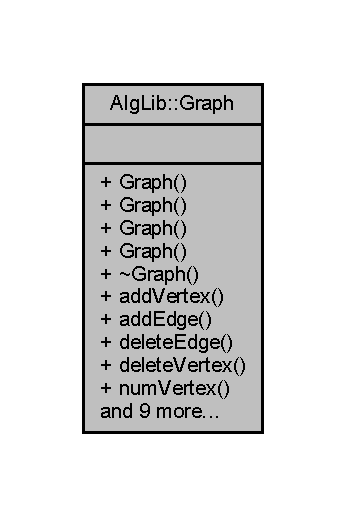
\includegraphics[width=166pt]{class_alg_lib_1_1_graph__coll__graph}
\end{center}
\end{figure}
\subsection*{Public Member Functions}
\begin{DoxyCompactItemize}
\item 
\hyperlink{class_alg_lib_1_1_graph_a365631724157558b77009a33f08104bd}{Graph} (int num\+Vertices, \hyperlink{namespace_alg_lib_a11966d2ea6c430adfb83a6ebaa05e337}{db\+Type} storage\+Type=\hyperlink{namespace_alg_lib_a11966d2ea6c430adfb83a6ebaa05e337a9d8e68c3898f769422174fed0be93fd2}{db\+Type\+::\+A\+D\+J\+A\+C\+E\+N\+C\+Y\+\_\+\+M\+A\+T\+R\+IX})
\begin{DoxyCompactList}\small\item\em A constructor. \end{DoxyCompactList}\item 
\hyperlink{class_alg_lib_1_1_graph_a99e286da01db1f3e8130cbef8ead77d5}{Graph} (const std\+::vector$<$ std\+::tuple$<$ int, int, double $>$ $>$ \&edgepairs, \hyperlink{namespace_alg_lib_a11966d2ea6c430adfb83a6ebaa05e337}{db\+Type} storage\+Type=\hyperlink{namespace_alg_lib_a11966d2ea6c430adfb83a6ebaa05e337a6d02e698876f8aa2b2e975e8c0010c10}{db\+Type\+::\+A\+D\+J\+A\+C\+E\+N\+C\+Y\+\_\+\+L\+I\+ST})
\begin{DoxyCompactList}\small\item\em A constructor that takes in edge pairs. \end{DoxyCompactList}\item 
\hyperlink{class_alg_lib_1_1_graph_a0cc9e7a1ff569edc8c019a5f2d9e4ee8}{Graph} (const \hyperlink{class_alg_lib_1_1_matrix}{Matrix}$<$ double $>$ \&adj\+Mat, \hyperlink{namespace_alg_lib_a11966d2ea6c430adfb83a6ebaa05e337}{db\+Type} storage\+Type=\hyperlink{namespace_alg_lib_a11966d2ea6c430adfb83a6ebaa05e337a9d8e68c3898f769422174fed0be93fd2}{db\+Type\+::\+A\+D\+J\+A\+C\+E\+N\+C\+Y\+\_\+\+M\+A\+T\+R\+IX})
\begin{DoxyCompactList}\small\item\em Constructor that takes in an adjacency matrix. \end{DoxyCompactList}\item 
\hyperlink{class_alg_lib_1_1_graph_abeb1fbb52b7f9ed8346f085b935fb7a8}{Graph} (const std\+::vector$<$ std\+::vector$<$ std\+::tuple$<$ int, double $>$ $>$ $>$ \&in\+Adj\+List, \hyperlink{namespace_alg_lib_a11966d2ea6c430adfb83a6ebaa05e337}{db\+Type} storage\+Type=\hyperlink{namespace_alg_lib_a11966d2ea6c430adfb83a6ebaa05e337a6d02e698876f8aa2b2e975e8c0010c10}{db\+Type\+::\+A\+D\+J\+A\+C\+E\+N\+C\+Y\+\_\+\+L\+I\+ST})
\begin{DoxyCompactList}\small\item\em Takes in an adjacency list to construct a graph. \end{DoxyCompactList}\item 
virtual \hyperlink{class_alg_lib_1_1_graph_a32cc4dfc6d81626b0175a237b0f2f765}{$\sim$\+Graph} ()
\item 
virtual void \hyperlink{class_alg_lib_1_1_graph_a48bb6066d823827bf8f030b528383b0a}{add\+Vertex} ()
\begin{DoxyCompactList}\small\item\em Adds a vertex to the graph. \end{DoxyCompactList}\item 
virtual void \hyperlink{class_alg_lib_1_1_graph_af5d14ec7c8cda4468f19777c612fce36}{add\+Edge} (int nodeS, int nodeE, double weight=1)
\begin{DoxyCompactList}\small\item\em Adds the edge nodeS -\/$>$ nodeE with the indicated weight. \end{DoxyCompactList}\item 
virtual void \hyperlink{class_alg_lib_1_1_graph_a7d92680925dcacb3761cf1c0cfd375a1}{delete\+Edge} (int nodeS, int nodeE)
\begin{DoxyCompactList}\small\item\em deletes the edge node\+S-\/$>$nodeE (really just sets the weight to 0) \end{DoxyCompactList}\item 
virtual void \hyperlink{class_alg_lib_1_1_graph_a44e68263784ec1eac40136fb2880b27f}{delete\+Vertex} (int node)
\begin{DoxyCompactList}\small\item\em Deletes the vertex numbered \char`\"{}node\char`\"{}. \end{DoxyCompactList}\item 
virtual int \hyperlink{class_alg_lib_1_1_graph_ad755bcd2eb09640252df1b137e18d129}{num\+Vertex} () const 
\begin{DoxyCompactList}\small\item\em Gives the number of vertices in the graph. \end{DoxyCompactList}\item 
virtual int \hyperlink{class_alg_lib_1_1_graph_afcf119c74be1f705e76929fcdf8c6532}{highest\+Node} () const 
\begin{DoxyCompactList}\small\item\em Returns the highest numbered node. \end{DoxyCompactList}\item 
virtual int \hyperlink{class_alg_lib_1_1_graph_af0d0a75b2003e433cc1f78cc2d528de6}{in\+Degree} (int node) const 
\begin{DoxyCompactList}\small\item\em Counts the number of edges going into a node. \end{DoxyCompactList}\item 
virtual int \hyperlink{class_alg_lib_1_1_graph_afd5a7862e0d564d4eb35bccae5b13d75}{out\+Degree} (int node) const 
\begin{DoxyCompactList}\small\item\em Counts the number of edges going out of a node. \end{DoxyCompactList}\item 
virtual double \hyperlink{class_alg_lib_1_1_graph_a320cb53252cef3ea2f1995dde174c727}{in\+Weight} (int node) const 
\begin{DoxyCompactList}\small\item\em Gives the total weight going into a node. \end{DoxyCompactList}\item 
virtual double \hyperlink{class_alg_lib_1_1_graph_ad0d722ed1e8530d3b6cdfa2224facb84}{out\+Weight} (int node) const 
\begin{DoxyCompactList}\small\item\em Gives the total weight going out of a node. \end{DoxyCompactList}\item 
virtual double \hyperlink{class_alg_lib_1_1_graph_acecdf6452fd10b763e8e9af300126771}{get\+Weight} (int nodeS, int nodeE) const 
\begin{DoxyCompactList}\small\item\em Returns the weight of edge node\+S-\/$>$nodeE. \end{DoxyCompactList}\item 
virtual bool \hyperlink{class_alg_lib_1_1_graph_a9b503efefa9c45a6acc9933a3502283c}{in\+Graph} (int node) const 
\begin{DoxyCompactList}\small\item\em A bool value of whether the number node is in the graph. \end{DoxyCompactList}\item 
virtual std\+::vector$<$ std\+::tuple$<$ int, double $>$ $>$ \hyperlink{class_alg_lib_1_1_graph_ab7c03a0caa842c589334c3a4aaaf4746}{out\+Adj} (int node) const 
\begin{DoxyCompactList}\small\item\em Gives the tuples with nodes x such that node-\/$>$x. \end{DoxyCompactList}\item 
virtual std\+::vector$<$ std\+::tuple$<$ int, double $>$ $>$ \hyperlink{class_alg_lib_1_1_graph_a59f621c5416a42b2b040b7bdd2d6b453}{in\+Adj} (int node) const 
\begin{DoxyCompactList}\small\item\em Gives the tuples with nodes x such that x-\/$>$node. \end{DoxyCompactList}\end{DoxyCompactItemize}


\subsection{Detailed Description}


Definition at line 15 of file Graph.\+h.



\subsection{Constructor \& Destructor Documentation}
\index{Alg\+Lib\+::\+Graph@{Alg\+Lib\+::\+Graph}!Graph@{Graph}}
\index{Graph@{Graph}!Alg\+Lib\+::\+Graph@{Alg\+Lib\+::\+Graph}}
\subsubsection[{\texorpdfstring{Graph(int num\+Vertices, db\+Type storage\+Type=db\+Type\+::\+A\+D\+J\+A\+C\+E\+N\+C\+Y\+\_\+\+M\+A\+T\+R\+I\+X)}{Graph(int numVertices, dbType storageType=dbType::ADJACENCY_MATRIX)}}]{\setlength{\rightskip}{0pt plus 5cm}Alg\+Lib\+::\+Graph\+::\+Graph (
\begin{DoxyParamCaption}
\item[{int}]{num\+Vertices, }
\item[{{\bf db\+Type}}]{storage\+Type = {\ttfamily {\bf db\+Type\+::\+A\+D\+J\+A\+C\+E\+N\+C\+Y\+\_\+\+M\+A\+T\+R\+IX}}}
\end{DoxyParamCaption}
)}\hypertarget{class_alg_lib_1_1_graph_a365631724157558b77009a33f08104bd}{}\label{class_alg_lib_1_1_graph_a365631724157558b77009a33f08104bd}


A constructor. 


\begin{DoxyParams}{Parameters}
{\em num\+Vertices} & the number of vertices for the graph to have \\
\hline
{\em storage\+Type} & an optional parameter about how the graph should be stored. \\
\hline
\end{DoxyParams}
\begin{DoxySeeAlso}{See also}
\hyperlink{namespace_alg_lib_a11966d2ea6c430adfb83a6ebaa05e337}{db\+Type} for more information on the types of graph databases available 
\end{DoxySeeAlso}


Definition at line 12 of file Graph.\+cpp.

\index{Alg\+Lib\+::\+Graph@{Alg\+Lib\+::\+Graph}!Graph@{Graph}}
\index{Graph@{Graph}!Alg\+Lib\+::\+Graph@{Alg\+Lib\+::\+Graph}}
\subsubsection[{\texorpdfstring{Graph(const std\+::vector$<$ std\+::tuple$<$ int, int, double $>$ $>$ \&edgepairs, db\+Type storage\+Type=db\+Type\+::\+A\+D\+J\+A\+C\+E\+N\+C\+Y\+\_\+\+L\+I\+S\+T)}{Graph(const std::vector< std::tuple< int, int, double > > &edgepairs, dbType storageType=dbType::ADJACENCY_LIST)}}]{\setlength{\rightskip}{0pt plus 5cm}Alg\+Lib\+::\+Graph\+::\+Graph (
\begin{DoxyParamCaption}
\item[{const std\+::vector$<$ std\+::tuple$<$ int, int, double $>$ $>$ \&}]{edgepairs, }
\item[{{\bf db\+Type}}]{storage\+Type = {\ttfamily {\bf db\+Type\+::\+A\+D\+J\+A\+C\+E\+N\+C\+Y\+\_\+\+L\+I\+ST}}}
\end{DoxyParamCaption}
)}\hypertarget{class_alg_lib_1_1_graph_a99e286da01db1f3e8130cbef8ead77d5}{}\label{class_alg_lib_1_1_graph_a99e286da01db1f3e8130cbef8ead77d5}


A constructor that takes in edge pairs. 


\begin{DoxyParams}{Parameters}
{\em edgepairs} & a vector containing tuples of the form (node1, node2, edgeweight) which will denote an edge from node1 to node 2 with weight edgeweight \\
\hline
{\em storage\+Type} & an optional parameter about how the graph should be stored. \\
\hline
\end{DoxyParams}
\begin{DoxySeeAlso}{See also}
\hyperlink{namespace_alg_lib_a11966d2ea6c430adfb83a6ebaa05e337}{db\+Type} for more information on the types of graph databases available 
\end{DoxySeeAlso}
\index{Alg\+Lib\+::\+Graph@{Alg\+Lib\+::\+Graph}!Graph@{Graph}}
\index{Graph@{Graph}!Alg\+Lib\+::\+Graph@{Alg\+Lib\+::\+Graph}}
\subsubsection[{\texorpdfstring{Graph(const Matrix$<$ double $>$ \&adj\+Mat, db\+Type storage\+Type=db\+Type\+::\+A\+D\+J\+A\+C\+E\+N\+C\+Y\+\_\+\+M\+A\+T\+R\+I\+X)}{Graph(const Matrix< double > &adjMat, dbType storageType=dbType::ADJACENCY_MATRIX)}}]{\setlength{\rightskip}{0pt plus 5cm}Alg\+Lib\+::\+Graph\+::\+Graph (
\begin{DoxyParamCaption}
\item[{const {\bf Matrix}$<$ double $>$ \&}]{adj\+Mat, }
\item[{{\bf db\+Type}}]{storage\+Type = {\ttfamily {\bf db\+Type\+::\+A\+D\+J\+A\+C\+E\+N\+C\+Y\+\_\+\+M\+A\+T\+R\+IX}}}
\end{DoxyParamCaption}
)}\hypertarget{class_alg_lib_1_1_graph_a0cc9e7a1ff569edc8c019a5f2d9e4ee8}{}\label{class_alg_lib_1_1_graph_a0cc9e7a1ff569edc8c019a5f2d9e4ee8}


Constructor that takes in an adjacency matrix. 


\begin{DoxyParams}{Parameters}
{\em adj\+Mat} & the adjacency matrix to take in. Edge i-\/$>$j with weight adj\+Mat\mbox{[}i\mbox{]}\mbox{[}j\mbox{]} \\
\hline
{\em storage\+Type} & an optional parameter about how the graph should be stored \\
\hline
\end{DoxyParams}
\begin{DoxySeeAlso}{See also}
\hyperlink{namespace_alg_lib_a11966d2ea6c430adfb83a6ebaa05e337}{db\+Type} for more information on the types of graph databases available 
\end{DoxySeeAlso}


Definition at line 53 of file Graph.\+cpp.

\index{Alg\+Lib\+::\+Graph@{Alg\+Lib\+::\+Graph}!Graph@{Graph}}
\index{Graph@{Graph}!Alg\+Lib\+::\+Graph@{Alg\+Lib\+::\+Graph}}
\subsubsection[{\texorpdfstring{Graph(const std\+::vector$<$ std\+::vector$<$ std\+::tuple$<$ int, double $>$ $>$ $>$ \&in\+Adj\+List, db\+Type storage\+Type=db\+Type\+::\+A\+D\+J\+A\+C\+E\+N\+C\+Y\+\_\+\+L\+I\+S\+T)}{Graph(const std::vector< std::vector< std::tuple< int, double > > > &inAdjList, dbType storageType=dbType::ADJACENCY_LIST)}}]{\setlength{\rightskip}{0pt plus 5cm}Alg\+Lib\+::\+Graph\+::\+Graph (
\begin{DoxyParamCaption}
\item[{const std\+::vector$<$ std\+::vector$<$ std\+::tuple$<$ int, double $>$ $>$ $>$ \&}]{in\+Adj\+List, }
\item[{{\bf db\+Type}}]{storage\+Type = {\ttfamily {\bf db\+Type\+::\+A\+D\+J\+A\+C\+E\+N\+C\+Y\+\_\+\+L\+I\+ST}}}
\end{DoxyParamCaption}
)}\hypertarget{class_alg_lib_1_1_graph_abeb1fbb52b7f9ed8346f085b935fb7a8}{}\label{class_alg_lib_1_1_graph_abeb1fbb52b7f9ed8346f085b935fb7a8}


Takes in an adjacency list to construct a graph. 


\begin{DoxyParams}{Parameters}
{\em in\+Adj\+List} & the adjacency list to take in. \\
\hline
{\em storage\+Type} & optional parameter about how the graph should be stored \\
\hline
\end{DoxyParams}
\begin{DoxySeeAlso}{See also}
\hyperlink{namespace_alg_lib_a11966d2ea6c430adfb83a6ebaa05e337}{db\+Type} for more information on the types of graph databases available 
\end{DoxySeeAlso}
\index{Alg\+Lib\+::\+Graph@{Alg\+Lib\+::\+Graph}!````~Graph@{$\sim$\+Graph}}
\index{````~Graph@{$\sim$\+Graph}!Alg\+Lib\+::\+Graph@{Alg\+Lib\+::\+Graph}}
\subsubsection[{\texorpdfstring{$\sim$\+Graph()}{~Graph()}}]{\setlength{\rightskip}{0pt plus 5cm}Alg\+Lib\+::\+Graph\+::$\sim$\+Graph (
\begin{DoxyParamCaption}
{}
\end{DoxyParamCaption}
)\hspace{0.3cm}{\ttfamily [virtual]}}\hypertarget{class_alg_lib_1_1_graph_a32cc4dfc6d81626b0175a237b0f2f765}{}\label{class_alg_lib_1_1_graph_a32cc4dfc6d81626b0175a237b0f2f765}
Default destructor 

Definition at line 103 of file Graph.\+cpp.



\subsection{Member Function Documentation}
\index{Alg\+Lib\+::\+Graph@{Alg\+Lib\+::\+Graph}!add\+Edge@{add\+Edge}}
\index{add\+Edge@{add\+Edge}!Alg\+Lib\+::\+Graph@{Alg\+Lib\+::\+Graph}}
\subsubsection[{\texorpdfstring{add\+Edge(int node\+S, int node\+E, double weight=1)}{addEdge(int nodeS, int nodeE, double weight=1)}}]{\setlength{\rightskip}{0pt plus 5cm}void Alg\+Lib\+::\+Graph\+::add\+Edge (
\begin{DoxyParamCaption}
\item[{int}]{nodeS, }
\item[{int}]{nodeE, }
\item[{double}]{weight = {\ttfamily 1}}
\end{DoxyParamCaption}
)\hspace{0.3cm}{\ttfamily [virtual]}}\hypertarget{class_alg_lib_1_1_graph_af5d14ec7c8cda4468f19777c612fce36}{}\label{class_alg_lib_1_1_graph_af5d14ec7c8cda4468f19777c612fce36}


Adds the edge nodeS -\/$>$ nodeE with the indicated weight. 


\begin{DoxyParams}{Parameters}
{\em nodeS} & the first node (the start) \\
\hline
{\em nodeE} & the second node (the end) \\
\hline
{\em weight} & the weight of the edge node\+S-\/$>$nodeE\\
\hline
\end{DoxyParams}
This will create a directed edge from nodeS to nodeE with weight 

Definition at line 114 of file Graph.\+cpp.

\index{Alg\+Lib\+::\+Graph@{Alg\+Lib\+::\+Graph}!add\+Vertex@{add\+Vertex}}
\index{add\+Vertex@{add\+Vertex}!Alg\+Lib\+::\+Graph@{Alg\+Lib\+::\+Graph}}
\subsubsection[{\texorpdfstring{add\+Vertex()}{addVertex()}}]{\setlength{\rightskip}{0pt plus 5cm}void Alg\+Lib\+::\+Graph\+::add\+Vertex (
\begin{DoxyParamCaption}
{}
\end{DoxyParamCaption}
)\hspace{0.3cm}{\ttfamily [virtual]}}\hypertarget{class_alg_lib_1_1_graph_a48bb6066d823827bf8f030b528383b0a}{}\label{class_alg_lib_1_1_graph_a48bb6066d823827bf8f030b528383b0a}


Adds a vertex to the graph. 

The node number that is added is the graph\textquotesingle{}s highest node number + 1, regardless of whether other nodes deleted. 

Definition at line 109 of file Graph.\+cpp.

\index{Alg\+Lib\+::\+Graph@{Alg\+Lib\+::\+Graph}!delete\+Edge@{delete\+Edge}}
\index{delete\+Edge@{delete\+Edge}!Alg\+Lib\+::\+Graph@{Alg\+Lib\+::\+Graph}}
\subsubsection[{\texorpdfstring{delete\+Edge(int node\+S, int node\+E)}{deleteEdge(int nodeS, int nodeE)}}]{\setlength{\rightskip}{0pt plus 5cm}void Alg\+Lib\+::\+Graph\+::delete\+Edge (
\begin{DoxyParamCaption}
\item[{int}]{nodeS, }
\item[{int}]{nodeE}
\end{DoxyParamCaption}
)\hspace{0.3cm}{\ttfamily [virtual]}}\hypertarget{class_alg_lib_1_1_graph_a7d92680925dcacb3761cf1c0cfd375a1}{}\label{class_alg_lib_1_1_graph_a7d92680925dcacb3761cf1c0cfd375a1}


deletes the edge node\+S-\/$>$nodeE (really just sets the weight to 0) 


\begin{DoxyParams}{Parameters}
{\em nodeS} & the first node of the edge \\
\hline
{\em nodeE} & the second node of the edge\\
\hline
\end{DoxyParams}
The edge is set to 0. It is no longer considered and adjacent edge of nodeS and nodeE 

Definition at line 119 of file Graph.\+cpp.

\index{Alg\+Lib\+::\+Graph@{Alg\+Lib\+::\+Graph}!delete\+Vertex@{delete\+Vertex}}
\index{delete\+Vertex@{delete\+Vertex}!Alg\+Lib\+::\+Graph@{Alg\+Lib\+::\+Graph}}
\subsubsection[{\texorpdfstring{delete\+Vertex(int node)}{deleteVertex(int node)}}]{\setlength{\rightskip}{0pt plus 5cm}void Alg\+Lib\+::\+Graph\+::delete\+Vertex (
\begin{DoxyParamCaption}
\item[{int}]{node}
\end{DoxyParamCaption}
)\hspace{0.3cm}{\ttfamily [virtual]}}\hypertarget{class_alg_lib_1_1_graph_a44e68263784ec1eac40136fb2880b27f}{}\label{class_alg_lib_1_1_graph_a44e68263784ec1eac40136fb2880b27f}


Deletes the vertex numbered \char`\"{}node\char`\"{}. 


\begin{DoxyParams}{Parameters}
{\em node} & The node to be removed\\
\hline
\end{DoxyParams}
The removal of this vertex will not affect the numbering of the nodes. It will simply be recorded that the node is not in the graph anymore. 

Definition at line 124 of file Graph.\+cpp.

\index{Alg\+Lib\+::\+Graph@{Alg\+Lib\+::\+Graph}!get\+Weight@{get\+Weight}}
\index{get\+Weight@{get\+Weight}!Alg\+Lib\+::\+Graph@{Alg\+Lib\+::\+Graph}}
\subsubsection[{\texorpdfstring{get\+Weight(int node\+S, int node\+E) const }{getWeight(int nodeS, int nodeE) const }}]{\setlength{\rightskip}{0pt plus 5cm}double Alg\+Lib\+::\+Graph\+::get\+Weight (
\begin{DoxyParamCaption}
\item[{int}]{nodeS, }
\item[{int}]{nodeE}
\end{DoxyParamCaption}
) const\hspace{0.3cm}{\ttfamily [virtual]}}\hypertarget{class_alg_lib_1_1_graph_acecdf6452fd10b763e8e9af300126771}{}\label{class_alg_lib_1_1_graph_acecdf6452fd10b763e8e9af300126771}


Returns the weight of edge node\+S-\/$>$nodeE. 


\begin{DoxyParams}{Parameters}
{\em nodeS} & the first node \\
\hline
{\em nodeE} & the second node \\
\hline
\end{DoxyParams}
\begin{DoxyReturn}{Returns}
the weight of edge node\+S-\/$>$nodeE 
\end{DoxyReturn}


Definition at line 159 of file Graph.\+cpp.

\index{Alg\+Lib\+::\+Graph@{Alg\+Lib\+::\+Graph}!highest\+Node@{highest\+Node}}
\index{highest\+Node@{highest\+Node}!Alg\+Lib\+::\+Graph@{Alg\+Lib\+::\+Graph}}
\subsubsection[{\texorpdfstring{highest\+Node() const }{highestNode() const }}]{\setlength{\rightskip}{0pt plus 5cm}int Alg\+Lib\+::\+Graph\+::highest\+Node (
\begin{DoxyParamCaption}
{}
\end{DoxyParamCaption}
) const\hspace{0.3cm}{\ttfamily [virtual]}}\hypertarget{class_alg_lib_1_1_graph_afcf119c74be1f705e76929fcdf8c6532}{}\label{class_alg_lib_1_1_graph_afcf119c74be1f705e76929fcdf8c6532}


Returns the highest numbered node. 

\begin{DoxyReturn}{Returns}
The highest numbered node in the graph. 
\end{DoxyReturn}
\begin{DoxySeeAlso}{See also}
\hyperlink{class_alg_lib_1_1_graph_ad755bcd2eb09640252df1b137e18d129}{num\+Vertex()} to find the number of ways to get the number of nodes 
\end{DoxySeeAlso}


Definition at line 134 of file Graph.\+cpp.

\index{Alg\+Lib\+::\+Graph@{Alg\+Lib\+::\+Graph}!in\+Adj@{in\+Adj}}
\index{in\+Adj@{in\+Adj}!Alg\+Lib\+::\+Graph@{Alg\+Lib\+::\+Graph}}
\subsubsection[{\texorpdfstring{in\+Adj(int node) const }{inAdj(int node) const }}]{\setlength{\rightskip}{0pt plus 5cm}std\+::vector$<$ std\+::tuple$<$ int, double $>$ $>$ Alg\+Lib\+::\+Graph\+::in\+Adj (
\begin{DoxyParamCaption}
\item[{int}]{node}
\end{DoxyParamCaption}
) const\hspace{0.3cm}{\ttfamily [virtual]}}\hypertarget{class_alg_lib_1_1_graph_a59f621c5416a42b2b040b7bdd2d6b453}{}\label{class_alg_lib_1_1_graph_a59f621c5416a42b2b040b7bdd2d6b453}


Gives the tuples with nodes x such that x-\/$>$node. 


\begin{DoxyParams}{Parameters}
{\em node} & The sink node\\
\hline
\end{DoxyParams}
\begin{DoxyReturn}{Returns}
A std\+::vector of std\+::tuple$<$int, double$>$ where the int is the connected node and double is the weight of the edge 
\end{DoxyReturn}


Definition at line 174 of file Graph.\+cpp.

\index{Alg\+Lib\+::\+Graph@{Alg\+Lib\+::\+Graph}!in\+Degree@{in\+Degree}}
\index{in\+Degree@{in\+Degree}!Alg\+Lib\+::\+Graph@{Alg\+Lib\+::\+Graph}}
\subsubsection[{\texorpdfstring{in\+Degree(int node) const }{inDegree(int node) const }}]{\setlength{\rightskip}{0pt plus 5cm}int Alg\+Lib\+::\+Graph\+::in\+Degree (
\begin{DoxyParamCaption}
\item[{int}]{node}
\end{DoxyParamCaption}
) const\hspace{0.3cm}{\ttfamily [virtual]}}\hypertarget{class_alg_lib_1_1_graph_af0d0a75b2003e433cc1f78cc2d528de6}{}\label{class_alg_lib_1_1_graph_af0d0a75b2003e433cc1f78cc2d528de6}


Counts the number of edges going into a node. 


\begin{DoxyParams}{Parameters}
{\em node} & The node\\
\hline
\end{DoxyParams}
\begin{DoxyReturn}{Returns}
The number of non zero directed edges going into that node 
\end{DoxyReturn}


Definition at line 139 of file Graph.\+cpp.

\index{Alg\+Lib\+::\+Graph@{Alg\+Lib\+::\+Graph}!in\+Graph@{in\+Graph}}
\index{in\+Graph@{in\+Graph}!Alg\+Lib\+::\+Graph@{Alg\+Lib\+::\+Graph}}
\subsubsection[{\texorpdfstring{in\+Graph(int node) const }{inGraph(int node) const }}]{\setlength{\rightskip}{0pt plus 5cm}bool Alg\+Lib\+::\+Graph\+::in\+Graph (
\begin{DoxyParamCaption}
\item[{int}]{node}
\end{DoxyParamCaption}
) const\hspace{0.3cm}{\ttfamily [virtual]}}\hypertarget{class_alg_lib_1_1_graph_a9b503efefa9c45a6acc9933a3502283c}{}\label{class_alg_lib_1_1_graph_a9b503efefa9c45a6acc9933a3502283c}


A bool value of whether the number node is in the graph. 


\begin{DoxyParams}{Parameters}
{\em node} & The number to see if it is a node in the graph\\
\hline
\end{DoxyParams}
\begin{DoxyReturn}{Returns}
True if node is in the graph, false otherwise. 
\end{DoxyReturn}


Definition at line 164 of file Graph.\+cpp.

\index{Alg\+Lib\+::\+Graph@{Alg\+Lib\+::\+Graph}!in\+Weight@{in\+Weight}}
\index{in\+Weight@{in\+Weight}!Alg\+Lib\+::\+Graph@{Alg\+Lib\+::\+Graph}}
\subsubsection[{\texorpdfstring{in\+Weight(int node) const }{inWeight(int node) const }}]{\setlength{\rightskip}{0pt plus 5cm}double Alg\+Lib\+::\+Graph\+::in\+Weight (
\begin{DoxyParamCaption}
\item[{int}]{node}
\end{DoxyParamCaption}
) const\hspace{0.3cm}{\ttfamily [virtual]}}\hypertarget{class_alg_lib_1_1_graph_a320cb53252cef3ea2f1995dde174c727}{}\label{class_alg_lib_1_1_graph_a320cb53252cef3ea2f1995dde174c727}


Gives the total weight going into a node. 


\begin{DoxyParams}{Parameters}
{\em node} & The node\\
\hline
\end{DoxyParams}
\begin{DoxyReturn}{Returns}
The total weight going into {\ttfamily node} 
\end{DoxyReturn}


Definition at line 149 of file Graph.\+cpp.

\index{Alg\+Lib\+::\+Graph@{Alg\+Lib\+::\+Graph}!num\+Vertex@{num\+Vertex}}
\index{num\+Vertex@{num\+Vertex}!Alg\+Lib\+::\+Graph@{Alg\+Lib\+::\+Graph}}
\subsubsection[{\texorpdfstring{num\+Vertex() const }{numVertex() const }}]{\setlength{\rightskip}{0pt plus 5cm}int Alg\+Lib\+::\+Graph\+::num\+Vertex (
\begin{DoxyParamCaption}
{}
\end{DoxyParamCaption}
) const\hspace{0.3cm}{\ttfamily [virtual]}}\hypertarget{class_alg_lib_1_1_graph_ad755bcd2eb09640252df1b137e18d129}{}\label{class_alg_lib_1_1_graph_ad755bcd2eb09640252df1b137e18d129}


Gives the number of vertices in the graph. 

\begin{DoxyReturn}{Returns}
The number of vertices in the graph. Removed nodes are not counted 
\end{DoxyReturn}
\begin{DoxySeeAlso}{See also}
\hyperlink{class_alg_lib_1_1_graph_afcf119c74be1f705e76929fcdf8c6532}{highest\+Node()} for how to get the highest numbered node 
\end{DoxySeeAlso}


Definition at line 129 of file Graph.\+cpp.

\index{Alg\+Lib\+::\+Graph@{Alg\+Lib\+::\+Graph}!out\+Adj@{out\+Adj}}
\index{out\+Adj@{out\+Adj}!Alg\+Lib\+::\+Graph@{Alg\+Lib\+::\+Graph}}
\subsubsection[{\texorpdfstring{out\+Adj(int node) const }{outAdj(int node) const }}]{\setlength{\rightskip}{0pt plus 5cm}std\+::vector$<$ std\+::tuple$<$ int, double $>$ $>$ Alg\+Lib\+::\+Graph\+::out\+Adj (
\begin{DoxyParamCaption}
\item[{int}]{node}
\end{DoxyParamCaption}
) const\hspace{0.3cm}{\ttfamily [virtual]}}\hypertarget{class_alg_lib_1_1_graph_ab7c03a0caa842c589334c3a4aaaf4746}{}\label{class_alg_lib_1_1_graph_ab7c03a0caa842c589334c3a4aaaf4746}


Gives the tuples with nodes x such that node-\/$>$x. 


\begin{DoxyParams}{Parameters}
{\em node} & The source node\\
\hline
\end{DoxyParams}
\begin{DoxyReturn}{Returns}
A std\+::vector of std\+::tuple$<$int, double$>$ where the int is the connected node and double is the weight of the edge 
\end{DoxyReturn}


Definition at line 169 of file Graph.\+cpp.

\index{Alg\+Lib\+::\+Graph@{Alg\+Lib\+::\+Graph}!out\+Degree@{out\+Degree}}
\index{out\+Degree@{out\+Degree}!Alg\+Lib\+::\+Graph@{Alg\+Lib\+::\+Graph}}
\subsubsection[{\texorpdfstring{out\+Degree(int node) const }{outDegree(int node) const }}]{\setlength{\rightskip}{0pt plus 5cm}int Alg\+Lib\+::\+Graph\+::out\+Degree (
\begin{DoxyParamCaption}
\item[{int}]{node}
\end{DoxyParamCaption}
) const\hspace{0.3cm}{\ttfamily [virtual]}}\hypertarget{class_alg_lib_1_1_graph_afd5a7862e0d564d4eb35bccae5b13d75}{}\label{class_alg_lib_1_1_graph_afd5a7862e0d564d4eb35bccae5b13d75}


Counts the number of edges going out of a node. 


\begin{DoxyParams}{Parameters}
{\em node} & The node\\
\hline
\end{DoxyParams}
\begin{DoxyReturn}{Returns}
The number of non zero directed edges going out of that node 
\end{DoxyReturn}


Definition at line 144 of file Graph.\+cpp.

\index{Alg\+Lib\+::\+Graph@{Alg\+Lib\+::\+Graph}!out\+Weight@{out\+Weight}}
\index{out\+Weight@{out\+Weight}!Alg\+Lib\+::\+Graph@{Alg\+Lib\+::\+Graph}}
\subsubsection[{\texorpdfstring{out\+Weight(int node) const }{outWeight(int node) const }}]{\setlength{\rightskip}{0pt plus 5cm}double Alg\+Lib\+::\+Graph\+::out\+Weight (
\begin{DoxyParamCaption}
\item[{int}]{node}
\end{DoxyParamCaption}
) const\hspace{0.3cm}{\ttfamily [virtual]}}\hypertarget{class_alg_lib_1_1_graph_ad0d722ed1e8530d3b6cdfa2224facb84}{}\label{class_alg_lib_1_1_graph_ad0d722ed1e8530d3b6cdfa2224facb84}


Gives the total weight going out of a node. 


\begin{DoxyParams}{Parameters}
{\em node} & The node\\
\hline
\end{DoxyParams}
\begin{DoxyReturn}{Returns}
The total weight going out of {\ttfamily node} 
\end{DoxyReturn}


Definition at line 154 of file Graph.\+cpp.



The documentation for this class was generated from the following files\+:\begin{DoxyCompactItemize}
\item 
D\+:/\+Data/\+Desktop/\+Github/include/\hyperlink{_graph_8h}{Graph.\+h}\item 
D\+:/\+Data/\+Desktop/\+Github/src/\+Graph/\hyperlink{_graph_8cpp}{Graph.\+cpp}\end{DoxyCompactItemize}

\hypertarget{class_alg_lib_1_1graph_d_b}{}\section{Alg\+Lib\+:\+:graph\+DB Class Reference}
\label{class_alg_lib_1_1graph_d_b}\index{Alg\+Lib\+::graph\+DB@{Alg\+Lib\+::graph\+DB}}


{\ttfamily \#include $<$graph\+D\+B.\+h$>$}



Inheritance diagram for Alg\+Lib\+:\+:graph\+DB\+:\nopagebreak
\begin{figure}[H]
\begin{center}
\leavevmode
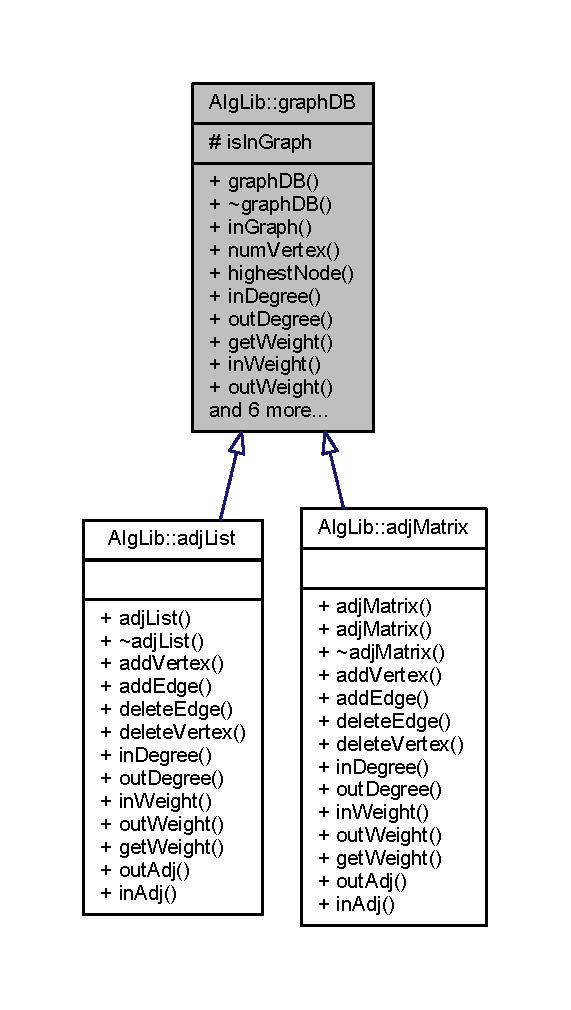
\includegraphics[width=274pt]{class_alg_lib_1_1graph_d_b__inherit__graph}
\end{center}
\end{figure}


Collaboration diagram for Alg\+Lib\+:\+:graph\+DB\+:\nopagebreak
\begin{figure}[H]
\begin{center}
\leavevmode
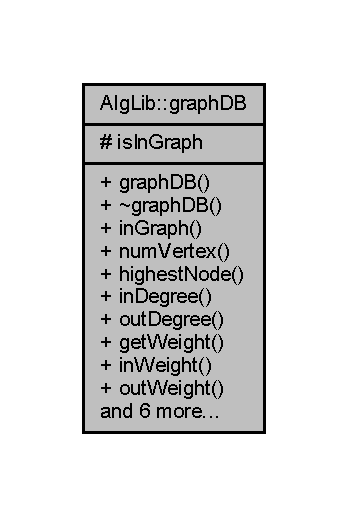
\includegraphics[width=167pt]{class_alg_lib_1_1graph_d_b__coll__graph}
\end{center}
\end{figure}
\subsection*{Public Member Functions}
\begin{DoxyCompactItemize}
\item 
\hyperlink{class_alg_lib_1_1graph_d_b_af5ab632982eda709108278a5153f6c70}{graph\+DB} (int num\+Vertices=0)
\item 
virtual \hyperlink{class_alg_lib_1_1graph_d_b_a58e8a1ab216494a97785fb21c7c344bc}{$\sim$graph\+DB} ()
\item 
virtual bool \hyperlink{class_alg_lib_1_1graph_d_b_ab897b7e45cbcfa65bf0c636630b52d93}{in\+Graph} (int node) const 
\item 
virtual int \hyperlink{class_alg_lib_1_1graph_d_b_a8d64de3b748352ed05aa0272c3a51195}{num\+Vertex} () const 
\item 
virtual int \hyperlink{class_alg_lib_1_1graph_d_b_a068476d8649ba9d30d32ed3f14dc2f6c}{highest\+Node} () const 
\item 
virtual int \hyperlink{class_alg_lib_1_1graph_d_b_a06faf4feb26d18b4491c5671158155f0}{in\+Degree} (int node) const  =0
\item 
virtual int \hyperlink{class_alg_lib_1_1graph_d_b_a8ac8d9aa118a2584d36d881f2f22a0c8}{out\+Degree} (int node) const  =0
\item 
virtual double \hyperlink{class_alg_lib_1_1graph_d_b_a8b81f180d935d1f80f728c0fef64ca03}{get\+Weight} (int nodeS, int nodeE) const  =0
\item 
virtual double \hyperlink{class_alg_lib_1_1graph_d_b_a873a4aa752f53702fad8cd36ab409c0e}{in\+Weight} (int node) const  =0
\item 
virtual double \hyperlink{class_alg_lib_1_1graph_d_b_a86dea18aed8b3bbcfaf834776d36f20f}{out\+Weight} (int node) const  =0
\item 
virtual std\+::vector$<$ std\+::tuple$<$ int, double $>$ $>$ \hyperlink{class_alg_lib_1_1graph_d_b_ae3c91d0775e8c2b28824a11f55571665}{out\+Adj} (int node) const  =0
\item 
virtual std\+::vector$<$ std\+::tuple$<$ int, double $>$ $>$ \hyperlink{class_alg_lib_1_1graph_d_b_abf67bacae3ae1faa4a9d5260f52ab1ca}{in\+Adj} (int node) const  =0
\item 
virtual void \hyperlink{class_alg_lib_1_1graph_d_b_abb3e87cafce37173f075c27c9c129554}{delete\+Vertex} (int node)=0
\item 
virtual void \hyperlink{class_alg_lib_1_1graph_d_b_a01fcc5af770b56fc187e40fb34ec9c9f}{delete\+Edge} (int nodeS, int nodeE)=0
\item 
virtual void \hyperlink{class_alg_lib_1_1graph_d_b_af21b1c41a94e6240b661bbe76f9fcb35}{add\+Vertex} ()=0
\item 
virtual void \hyperlink{class_alg_lib_1_1graph_d_b_aeedc15cdbef55a131d7cf3d91778032e}{add\+Edge} (int nodeS, int nodeE, double weight=1)=0
\end{DoxyCompactItemize}
\subsection*{Protected Attributes}
\begin{DoxyCompactItemize}
\item 
std\+::vector$<$ bool $>$ \hyperlink{class_alg_lib_1_1graph_d_b_adc2ea4ed0aec4a2cd22cbe292c4152ae}{is\+In\+Graph}
\end{DoxyCompactItemize}


\subsection{Detailed Description}


Definition at line 7 of file graph\+D\+B.\+h.



\subsection{Constructor \& Destructor Documentation}
\index{Alg\+Lib\+::graph\+DB@{Alg\+Lib\+::graph\+DB}!graph\+DB@{graph\+DB}}
\index{graph\+DB@{graph\+DB}!Alg\+Lib\+::graph\+DB@{Alg\+Lib\+::graph\+DB}}
\subsubsection[{\texorpdfstring{graph\+D\+B(int num\+Vertices=0)}{graphDB(int numVertices=0)}}]{\setlength{\rightskip}{0pt plus 5cm}Alg\+Lib\+::graph\+D\+B\+::graph\+DB (
\begin{DoxyParamCaption}
\item[{int}]{num\+Vertices = {\ttfamily 0}}
\end{DoxyParamCaption}
)}\hypertarget{class_alg_lib_1_1graph_d_b_af5ab632982eda709108278a5153f6c70}{}\label{class_alg_lib_1_1graph_d_b_af5ab632982eda709108278a5153f6c70}
Default constructor 

Definition at line 5 of file graph\+D\+B.\+cpp.

\index{Alg\+Lib\+::graph\+DB@{Alg\+Lib\+::graph\+DB}!````~graph\+DB@{$\sim$graph\+DB}}
\index{````~graph\+DB@{$\sim$graph\+DB}!Alg\+Lib\+::graph\+DB@{Alg\+Lib\+::graph\+DB}}
\subsubsection[{\texorpdfstring{$\sim$graph\+D\+B()}{~graphDB()}}]{\setlength{\rightskip}{0pt plus 5cm}Alg\+Lib\+::graph\+D\+B\+::$\sim$graph\+DB (
\begin{DoxyParamCaption}
{}
\end{DoxyParamCaption}
)\hspace{0.3cm}{\ttfamily [virtual]}}\hypertarget{class_alg_lib_1_1graph_d_b_a58e8a1ab216494a97785fb21c7c344bc}{}\label{class_alg_lib_1_1graph_d_b_a58e8a1ab216494a97785fb21c7c344bc}
Default destructor 

Definition at line 11 of file graph\+D\+B.\+cpp.



\subsection{Member Function Documentation}
\index{Alg\+Lib\+::graph\+DB@{Alg\+Lib\+::graph\+DB}!add\+Edge@{add\+Edge}}
\index{add\+Edge@{add\+Edge}!Alg\+Lib\+::graph\+DB@{Alg\+Lib\+::graph\+DB}}
\subsubsection[{\texorpdfstring{add\+Edge(int node\+S, int node\+E, double weight=1)=0}{addEdge(int nodeS, int nodeE, double weight=1)=0}}]{\setlength{\rightskip}{0pt plus 5cm}virtual void Alg\+Lib\+::graph\+D\+B\+::add\+Edge (
\begin{DoxyParamCaption}
\item[{int}]{nodeS, }
\item[{int}]{nodeE, }
\item[{double}]{weight = {\ttfamily 1}}
\end{DoxyParamCaption}
)\hspace{0.3cm}{\ttfamily [pure virtual]}}\hypertarget{class_alg_lib_1_1graph_d_b_aeedc15cdbef55a131d7cf3d91778032e}{}\label{class_alg_lib_1_1graph_d_b_aeedc15cdbef55a131d7cf3d91778032e}


Implemented in \hyperlink{class_alg_lib_1_1adj_matrix_a4ca87cc5146e1a1e8967a5cd358711cc}{Alg\+Lib\+::adj\+Matrix}, and \hyperlink{class_alg_lib_1_1adj_list_a1010763e586866d884ebb769df8fba52}{Alg\+Lib\+::adj\+List}.

\index{Alg\+Lib\+::graph\+DB@{Alg\+Lib\+::graph\+DB}!add\+Vertex@{add\+Vertex}}
\index{add\+Vertex@{add\+Vertex}!Alg\+Lib\+::graph\+DB@{Alg\+Lib\+::graph\+DB}}
\subsubsection[{\texorpdfstring{add\+Vertex()=0}{addVertex()=0}}]{\setlength{\rightskip}{0pt plus 5cm}virtual void Alg\+Lib\+::graph\+D\+B\+::add\+Vertex (
\begin{DoxyParamCaption}
{}
\end{DoxyParamCaption}
)\hspace{0.3cm}{\ttfamily [pure virtual]}}\hypertarget{class_alg_lib_1_1graph_d_b_af21b1c41a94e6240b661bbe76f9fcb35}{}\label{class_alg_lib_1_1graph_d_b_af21b1c41a94e6240b661bbe76f9fcb35}


Implemented in \hyperlink{class_alg_lib_1_1adj_matrix_a55d736fcb0d25028df7e4775d0b7fa53}{Alg\+Lib\+::adj\+Matrix}, and \hyperlink{class_alg_lib_1_1adj_list_a15380331b1b6b6b510052b5e43f4ba50}{Alg\+Lib\+::adj\+List}.

\index{Alg\+Lib\+::graph\+DB@{Alg\+Lib\+::graph\+DB}!delete\+Edge@{delete\+Edge}}
\index{delete\+Edge@{delete\+Edge}!Alg\+Lib\+::graph\+DB@{Alg\+Lib\+::graph\+DB}}
\subsubsection[{\texorpdfstring{delete\+Edge(int node\+S, int node\+E)=0}{deleteEdge(int nodeS, int nodeE)=0}}]{\setlength{\rightskip}{0pt plus 5cm}virtual void Alg\+Lib\+::graph\+D\+B\+::delete\+Edge (
\begin{DoxyParamCaption}
\item[{int}]{nodeS, }
\item[{int}]{nodeE}
\end{DoxyParamCaption}
)\hspace{0.3cm}{\ttfamily [pure virtual]}}\hypertarget{class_alg_lib_1_1graph_d_b_a01fcc5af770b56fc187e40fb34ec9c9f}{}\label{class_alg_lib_1_1graph_d_b_a01fcc5af770b56fc187e40fb34ec9c9f}


Implemented in \hyperlink{class_alg_lib_1_1adj_matrix_ac644ad4932439fea257938c42c7f6ec3}{Alg\+Lib\+::adj\+Matrix}, and \hyperlink{class_alg_lib_1_1adj_list_a11ced2c2ac3cc989e9c23c6e63dc41c5}{Alg\+Lib\+::adj\+List}.

\index{Alg\+Lib\+::graph\+DB@{Alg\+Lib\+::graph\+DB}!delete\+Vertex@{delete\+Vertex}}
\index{delete\+Vertex@{delete\+Vertex}!Alg\+Lib\+::graph\+DB@{Alg\+Lib\+::graph\+DB}}
\subsubsection[{\texorpdfstring{delete\+Vertex(int node)=0}{deleteVertex(int node)=0}}]{\setlength{\rightskip}{0pt plus 5cm}virtual void Alg\+Lib\+::graph\+D\+B\+::delete\+Vertex (
\begin{DoxyParamCaption}
\item[{int}]{node}
\end{DoxyParamCaption}
)\hspace{0.3cm}{\ttfamily [pure virtual]}}\hypertarget{class_alg_lib_1_1graph_d_b_abb3e87cafce37173f075c27c9c129554}{}\label{class_alg_lib_1_1graph_d_b_abb3e87cafce37173f075c27c9c129554}


Implemented in \hyperlink{class_alg_lib_1_1adj_matrix_a7e59572f5c9c80853364132cd92eb9a0}{Alg\+Lib\+::adj\+Matrix}, and \hyperlink{class_alg_lib_1_1adj_list_a37fa96194420fd556668dc8c4ce5472f}{Alg\+Lib\+::adj\+List}.

\index{Alg\+Lib\+::graph\+DB@{Alg\+Lib\+::graph\+DB}!get\+Weight@{get\+Weight}}
\index{get\+Weight@{get\+Weight}!Alg\+Lib\+::graph\+DB@{Alg\+Lib\+::graph\+DB}}
\subsubsection[{\texorpdfstring{get\+Weight(int node\+S, int node\+E) const  =0}{getWeight(int nodeS, int nodeE) const  =0}}]{\setlength{\rightskip}{0pt plus 5cm}virtual double Alg\+Lib\+::graph\+D\+B\+::get\+Weight (
\begin{DoxyParamCaption}
\item[{int}]{nodeS, }
\item[{int}]{nodeE}
\end{DoxyParamCaption}
) const\hspace{0.3cm}{\ttfamily [pure virtual]}}\hypertarget{class_alg_lib_1_1graph_d_b_a8b81f180d935d1f80f728c0fef64ca03}{}\label{class_alg_lib_1_1graph_d_b_a8b81f180d935d1f80f728c0fef64ca03}


Implemented in \hyperlink{class_alg_lib_1_1adj_matrix_a05bbb7b2b30f83c6b89ff75dc6cc84ea}{Alg\+Lib\+::adj\+Matrix}, and \hyperlink{class_alg_lib_1_1adj_list_a1f365ed028dd4bdce2fc47119f47dde7}{Alg\+Lib\+::adj\+List}.

\index{Alg\+Lib\+::graph\+DB@{Alg\+Lib\+::graph\+DB}!highest\+Node@{highest\+Node}}
\index{highest\+Node@{highest\+Node}!Alg\+Lib\+::graph\+DB@{Alg\+Lib\+::graph\+DB}}
\subsubsection[{\texorpdfstring{highest\+Node() const }{highestNode() const }}]{\setlength{\rightskip}{0pt plus 5cm}int Alg\+Lib\+::graph\+D\+B\+::highest\+Node (
\begin{DoxyParamCaption}
{}
\end{DoxyParamCaption}
) const\hspace{0.3cm}{\ttfamily [virtual]}}\hypertarget{class_alg_lib_1_1graph_d_b_a068476d8649ba9d30d32ed3f14dc2f6c}{}\label{class_alg_lib_1_1graph_d_b_a068476d8649ba9d30d32ed3f14dc2f6c}


Definition at line 34 of file graph\+D\+B.\+cpp.

\index{Alg\+Lib\+::graph\+DB@{Alg\+Lib\+::graph\+DB}!in\+Adj@{in\+Adj}}
\index{in\+Adj@{in\+Adj}!Alg\+Lib\+::graph\+DB@{Alg\+Lib\+::graph\+DB}}
\subsubsection[{\texorpdfstring{in\+Adj(int node) const  =0}{inAdj(int node) const  =0}}]{\setlength{\rightskip}{0pt plus 5cm}virtual std\+::vector$<$ std\+::tuple $<$int, double$>$ $>$ Alg\+Lib\+::graph\+D\+B\+::in\+Adj (
\begin{DoxyParamCaption}
\item[{int}]{node}
\end{DoxyParamCaption}
) const\hspace{0.3cm}{\ttfamily [pure virtual]}}\hypertarget{class_alg_lib_1_1graph_d_b_abf67bacae3ae1faa4a9d5260f52ab1ca}{}\label{class_alg_lib_1_1graph_d_b_abf67bacae3ae1faa4a9d5260f52ab1ca}


Implemented in \hyperlink{class_alg_lib_1_1adj_matrix_a52a5e7ac8fdd3bf11aa6dcf38d800ecb}{Alg\+Lib\+::adj\+Matrix}, and \hyperlink{class_alg_lib_1_1adj_list_a2f8f4af6435990aea3b90b3274bf64bf}{Alg\+Lib\+::adj\+List}.

\index{Alg\+Lib\+::graph\+DB@{Alg\+Lib\+::graph\+DB}!in\+Degree@{in\+Degree}}
\index{in\+Degree@{in\+Degree}!Alg\+Lib\+::graph\+DB@{Alg\+Lib\+::graph\+DB}}
\subsubsection[{\texorpdfstring{in\+Degree(int node) const  =0}{inDegree(int node) const  =0}}]{\setlength{\rightskip}{0pt plus 5cm}virtual int Alg\+Lib\+::graph\+D\+B\+::in\+Degree (
\begin{DoxyParamCaption}
\item[{int}]{node}
\end{DoxyParamCaption}
) const\hspace{0.3cm}{\ttfamily [pure virtual]}}\hypertarget{class_alg_lib_1_1graph_d_b_a06faf4feb26d18b4491c5671158155f0}{}\label{class_alg_lib_1_1graph_d_b_a06faf4feb26d18b4491c5671158155f0}


Implemented in \hyperlink{class_alg_lib_1_1adj_matrix_a50039a0fb126b3996b30e3b9fd8e7933}{Alg\+Lib\+::adj\+Matrix}, and \hyperlink{class_alg_lib_1_1adj_list_a73b55f7e622358e9ac4f2dbd076b393d}{Alg\+Lib\+::adj\+List}.

\index{Alg\+Lib\+::graph\+DB@{Alg\+Lib\+::graph\+DB}!in\+Graph@{in\+Graph}}
\index{in\+Graph@{in\+Graph}!Alg\+Lib\+::graph\+DB@{Alg\+Lib\+::graph\+DB}}
\subsubsection[{\texorpdfstring{in\+Graph(int node) const }{inGraph(int node) const }}]{\setlength{\rightskip}{0pt plus 5cm}bool Alg\+Lib\+::graph\+D\+B\+::in\+Graph (
\begin{DoxyParamCaption}
\item[{int}]{node}
\end{DoxyParamCaption}
) const\hspace{0.3cm}{\ttfamily [virtual]}}\hypertarget{class_alg_lib_1_1graph_d_b_ab897b7e45cbcfa65bf0c636630b52d93}{}\label{class_alg_lib_1_1graph_d_b_ab897b7e45cbcfa65bf0c636630b52d93}


Definition at line 16 of file graph\+D\+B.\+cpp.

\index{Alg\+Lib\+::graph\+DB@{Alg\+Lib\+::graph\+DB}!in\+Weight@{in\+Weight}}
\index{in\+Weight@{in\+Weight}!Alg\+Lib\+::graph\+DB@{Alg\+Lib\+::graph\+DB}}
\subsubsection[{\texorpdfstring{in\+Weight(int node) const  =0}{inWeight(int node) const  =0}}]{\setlength{\rightskip}{0pt plus 5cm}virtual double Alg\+Lib\+::graph\+D\+B\+::in\+Weight (
\begin{DoxyParamCaption}
\item[{int}]{node}
\end{DoxyParamCaption}
) const\hspace{0.3cm}{\ttfamily [pure virtual]}}\hypertarget{class_alg_lib_1_1graph_d_b_a873a4aa752f53702fad8cd36ab409c0e}{}\label{class_alg_lib_1_1graph_d_b_a873a4aa752f53702fad8cd36ab409c0e}


Implemented in \hyperlink{class_alg_lib_1_1adj_matrix_aab4ecb9801ba43d2ce3c0f542e44643e}{Alg\+Lib\+::adj\+Matrix}, and \hyperlink{class_alg_lib_1_1adj_list_a74fbc3342cdd18cfbd1a3c26982d03a0}{Alg\+Lib\+::adj\+List}.

\index{Alg\+Lib\+::graph\+DB@{Alg\+Lib\+::graph\+DB}!num\+Vertex@{num\+Vertex}}
\index{num\+Vertex@{num\+Vertex}!Alg\+Lib\+::graph\+DB@{Alg\+Lib\+::graph\+DB}}
\subsubsection[{\texorpdfstring{num\+Vertex() const }{numVertex() const }}]{\setlength{\rightskip}{0pt plus 5cm}int Alg\+Lib\+::graph\+D\+B\+::num\+Vertex (
\begin{DoxyParamCaption}
{}
\end{DoxyParamCaption}
) const\hspace{0.3cm}{\ttfamily [virtual]}}\hypertarget{class_alg_lib_1_1graph_d_b_a8d64de3b748352ed05aa0272c3a51195}{}\label{class_alg_lib_1_1graph_d_b_a8d64de3b748352ed05aa0272c3a51195}


Definition at line 23 of file graph\+D\+B.\+cpp.

\index{Alg\+Lib\+::graph\+DB@{Alg\+Lib\+::graph\+DB}!out\+Adj@{out\+Adj}}
\index{out\+Adj@{out\+Adj}!Alg\+Lib\+::graph\+DB@{Alg\+Lib\+::graph\+DB}}
\subsubsection[{\texorpdfstring{out\+Adj(int node) const  =0}{outAdj(int node) const  =0}}]{\setlength{\rightskip}{0pt plus 5cm}virtual std\+::vector$<$ std\+::tuple $<$int, double$>$ $>$ Alg\+Lib\+::graph\+D\+B\+::out\+Adj (
\begin{DoxyParamCaption}
\item[{int}]{node}
\end{DoxyParamCaption}
) const\hspace{0.3cm}{\ttfamily [pure virtual]}}\hypertarget{class_alg_lib_1_1graph_d_b_ae3c91d0775e8c2b28824a11f55571665}{}\label{class_alg_lib_1_1graph_d_b_ae3c91d0775e8c2b28824a11f55571665}


Implemented in \hyperlink{class_alg_lib_1_1adj_matrix_a0e8e97ad4fba9e2862d36ab1be2324f1}{Alg\+Lib\+::adj\+Matrix}, and \hyperlink{class_alg_lib_1_1adj_list_a01a7eb08e676f75a339403079e004e00}{Alg\+Lib\+::adj\+List}.

\index{Alg\+Lib\+::graph\+DB@{Alg\+Lib\+::graph\+DB}!out\+Degree@{out\+Degree}}
\index{out\+Degree@{out\+Degree}!Alg\+Lib\+::graph\+DB@{Alg\+Lib\+::graph\+DB}}
\subsubsection[{\texorpdfstring{out\+Degree(int node) const  =0}{outDegree(int node) const  =0}}]{\setlength{\rightskip}{0pt plus 5cm}virtual int Alg\+Lib\+::graph\+D\+B\+::out\+Degree (
\begin{DoxyParamCaption}
\item[{int}]{node}
\end{DoxyParamCaption}
) const\hspace{0.3cm}{\ttfamily [pure virtual]}}\hypertarget{class_alg_lib_1_1graph_d_b_a8ac8d9aa118a2584d36d881f2f22a0c8}{}\label{class_alg_lib_1_1graph_d_b_a8ac8d9aa118a2584d36d881f2f22a0c8}


Implemented in \hyperlink{class_alg_lib_1_1adj_matrix_afbe220e5939f2c5bb621b482904eeef0}{Alg\+Lib\+::adj\+Matrix}, and \hyperlink{class_alg_lib_1_1adj_list_a3bb70be60dc28fedf1817c76f5b881f2}{Alg\+Lib\+::adj\+List}.

\index{Alg\+Lib\+::graph\+DB@{Alg\+Lib\+::graph\+DB}!out\+Weight@{out\+Weight}}
\index{out\+Weight@{out\+Weight}!Alg\+Lib\+::graph\+DB@{Alg\+Lib\+::graph\+DB}}
\subsubsection[{\texorpdfstring{out\+Weight(int node) const  =0}{outWeight(int node) const  =0}}]{\setlength{\rightskip}{0pt plus 5cm}virtual double Alg\+Lib\+::graph\+D\+B\+::out\+Weight (
\begin{DoxyParamCaption}
\item[{int}]{node}
\end{DoxyParamCaption}
) const\hspace{0.3cm}{\ttfamily [pure virtual]}}\hypertarget{class_alg_lib_1_1graph_d_b_a86dea18aed8b3bbcfaf834776d36f20f}{}\label{class_alg_lib_1_1graph_d_b_a86dea18aed8b3bbcfaf834776d36f20f}


Implemented in \hyperlink{class_alg_lib_1_1adj_matrix_a3d807c32353c656f362ed356c4f3d1ed}{Alg\+Lib\+::adj\+Matrix}, and \hyperlink{class_alg_lib_1_1adj_list_aeeabf593091f0d068f77d5ed000ab06b}{Alg\+Lib\+::adj\+List}.



\subsection{Member Data Documentation}
\index{Alg\+Lib\+::graph\+DB@{Alg\+Lib\+::graph\+DB}!is\+In\+Graph@{is\+In\+Graph}}
\index{is\+In\+Graph@{is\+In\+Graph}!Alg\+Lib\+::graph\+DB@{Alg\+Lib\+::graph\+DB}}
\subsubsection[{\texorpdfstring{is\+In\+Graph}{isInGraph}}]{\setlength{\rightskip}{0pt plus 5cm}std\+::vector$<$bool$>$ Alg\+Lib\+::graph\+D\+B\+::is\+In\+Graph\hspace{0.3cm}{\ttfamily [protected]}}\hypertarget{class_alg_lib_1_1graph_d_b_adc2ea4ed0aec4a2cd22cbe292c4152ae}{}\label{class_alg_lib_1_1graph_d_b_adc2ea4ed0aec4a2cd22cbe292c4152ae}


Definition at line 35 of file graph\+D\+B.\+h.



The documentation for this class was generated from the following files\+:\begin{DoxyCompactItemize}
\item 
D\+:/\+Data/\+Desktop/\+Github/include/\hyperlink{graph_d_b_8h}{graph\+D\+B.\+h}\item 
D\+:/\+Data/\+Desktop/\+Github/src/\+Graph/\hyperlink{graph_d_b_8cpp}{graph\+D\+B.\+cpp}\end{DoxyCompactItemize}

\hypertarget{class_alg_lib_1_1_heap}{}\section{Alg\+Lib\+:\+:Heap$<$ T $>$ Class Template Reference}
\label{class_alg_lib_1_1_heap}\index{Alg\+Lib\+::\+Heap$<$ T $>$@{Alg\+Lib\+::\+Heap$<$ T $>$}}


{\ttfamily \#include $<$Heap.\+h$>$}



Collaboration diagram for Alg\+Lib\+:\+:Heap$<$ T $>$\+:\nopagebreak
\begin{figure}[H]
\begin{center}
\leavevmode
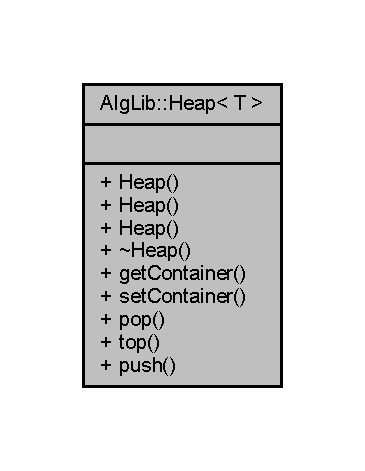
\includegraphics[width=175pt]{class_alg_lib_1_1_heap__coll__graph}
\end{center}
\end{figure}
\subsection*{Public Member Functions}
\begin{DoxyCompactItemize}
\item 
\hyperlink{class_alg_lib_1_1_heap_aba2cc050f886d9a8247f24347d9c9b55}{Heap} ()
\item 
\hyperlink{class_alg_lib_1_1_heap_a068f2a62a4468625b4ad14507a386fc8}{Heap} (std\+::vector$<$ T $>$ container)
\item 
\hyperlink{class_alg_lib_1_1_heap_a7b009e741c0442339eb54d992d3c74da}{Heap} (std\+::initializer\+\_\+list$<$ T $>$ args)
\begin{DoxyCompactList}\small\item\em (one liner) \end{DoxyCompactList}\item 
virtual \hyperlink{class_alg_lib_1_1_heap_a0d6a73495b76725db1d612050c090c73}{$\sim$\+Heap} ()
\item 
virtual std\+::vector$<$ T $>$ \hyperlink{class_alg_lib_1_1_heap_a26fff42a724f914607f61c25dc4f80bd}{get\+Container} ()
\item 
virtual void \hyperlink{class_alg_lib_1_1_heap_a0c406e0e00559e3372637d1547af1023}{set\+Container} (std\+::vector$<$ T $>$ val)
\item 
virtual T \hyperlink{class_alg_lib_1_1_heap_a827f1aa55e4d2b366e3c2e1753b2bb38}{pop} ()
\item 
virtual T \hyperlink{class_alg_lib_1_1_heap_a4f1ab496a7f4a4cc4d5c917fe10514ff}{top} ()
\item 
virtual void \hyperlink{class_alg_lib_1_1_heap_a37d97dc0bc90f4b1dedfaa3378133f89}{push} (T elem)
\begin{DoxyCompactList}\small\item\em (one liner) \end{DoxyCompactList}\end{DoxyCompactItemize}


\subsection{Detailed Description}
\subsubsection*{template$<$typename T$>$\\*
class Alg\+Lib\+::\+Heap$<$ T $>$}



Definition at line 9 of file Heap.\+h.



\subsection{Constructor \& Destructor Documentation}
\index{Alg\+Lib\+::\+Heap@{Alg\+Lib\+::\+Heap}!Heap@{Heap}}
\index{Heap@{Heap}!Alg\+Lib\+::\+Heap@{Alg\+Lib\+::\+Heap}}
\subsubsection[{\texorpdfstring{Heap()}{Heap()}}]{\setlength{\rightskip}{0pt plus 5cm}template$<$typename T $>$ {\bf Alg\+Lib\+::\+Heap}$<$ T $>$\+::{\bf Heap} (
\begin{DoxyParamCaption}
{}
\end{DoxyParamCaption}
)}\hypertarget{class_alg_lib_1_1_heap_aba2cc050f886d9a8247f24347d9c9b55}{}\label{class_alg_lib_1_1_heap_aba2cc050f886d9a8247f24347d9c9b55}
Default constructor 

Definition at line 8 of file Heap.\+cpp.

\index{Alg\+Lib\+::\+Heap@{Alg\+Lib\+::\+Heap}!Heap@{Heap}}
\index{Heap@{Heap}!Alg\+Lib\+::\+Heap@{Alg\+Lib\+::\+Heap}}
\subsubsection[{\texorpdfstring{Heap(std\+::vector$<$ T $>$ container)}{Heap(std::vector< T > container)}}]{\setlength{\rightskip}{0pt plus 5cm}template$<$typename T $>$ {\bf Alg\+Lib\+::\+Heap}$<$ T $>$\+::{\bf Heap} (
\begin{DoxyParamCaption}
\item[{std\+::vector$<$ T $>$}]{container}
\end{DoxyParamCaption}
)}\hypertarget{class_alg_lib_1_1_heap_a068f2a62a4468625b4ad14507a386fc8}{}\label{class_alg_lib_1_1_heap_a068f2a62a4468625b4ad14507a386fc8}
Constructor that takes in vector$<$\+T$>$ 

Definition at line 15 of file Heap.\+cpp.

\index{Alg\+Lib\+::\+Heap@{Alg\+Lib\+::\+Heap}!Heap@{Heap}}
\index{Heap@{Heap}!Alg\+Lib\+::\+Heap@{Alg\+Lib\+::\+Heap}}
\subsubsection[{\texorpdfstring{Heap(std\+::initializer\+\_\+list$<$ T $>$ args)}{Heap(std::initializer_list< T > args)}}]{\setlength{\rightskip}{0pt plus 5cm}template$<$typename T $>$ {\bf Alg\+Lib\+::\+Heap}$<$ T $>$\+::{\bf Heap} (
\begin{DoxyParamCaption}
\item[{std\+::initializer\+\_\+list$<$ T $>$}]{args}
\end{DoxyParamCaption}
)}\hypertarget{class_alg_lib_1_1_heap_a7b009e741c0442339eb54d992d3c74da}{}\label{class_alg_lib_1_1_heap_a7b009e741c0442339eb54d992d3c74da}


(one liner) 

Initializer list constructor

(documentation goes here) 

Definition at line 27 of file Heap.\+cpp.

\index{Alg\+Lib\+::\+Heap@{Alg\+Lib\+::\+Heap}!````~Heap@{$\sim$\+Heap}}
\index{````~Heap@{$\sim$\+Heap}!Alg\+Lib\+::\+Heap@{Alg\+Lib\+::\+Heap}}
\subsubsection[{\texorpdfstring{$\sim$\+Heap()}{~Heap()}}]{\setlength{\rightskip}{0pt plus 5cm}template$<$typename T $>$ {\bf Alg\+Lib\+::\+Heap}$<$ T $>$\+::$\sim${\bf Heap} (
\begin{DoxyParamCaption}
{}
\end{DoxyParamCaption}
)\hspace{0.3cm}{\ttfamily [virtual]}}\hypertarget{class_alg_lib_1_1_heap_a0d6a73495b76725db1d612050c090c73}{}\label{class_alg_lib_1_1_heap_a0d6a73495b76725db1d612050c090c73}
Default destructor 

Definition at line 60 of file Heap.\+cpp.



\subsection{Member Function Documentation}
\index{Alg\+Lib\+::\+Heap@{Alg\+Lib\+::\+Heap}!get\+Container@{get\+Container}}
\index{get\+Container@{get\+Container}!Alg\+Lib\+::\+Heap@{Alg\+Lib\+::\+Heap}}
\subsubsection[{\texorpdfstring{get\+Container()}{getContainer()}}]{\setlength{\rightskip}{0pt plus 5cm}template$<$typename T$>$ virtual std\+::vector$<$T$>$ {\bf Alg\+Lib\+::\+Heap}$<$ T $>$\+::get\+Container (
\begin{DoxyParamCaption}
{}
\end{DoxyParamCaption}
)\hspace{0.3cm}{\ttfamily [inline]}, {\ttfamily [virtual]}}\hypertarget{class_alg_lib_1_1_heap_a26fff42a724f914607f61c25dc4f80bd}{}\label{class_alg_lib_1_1_heap_a26fff42a724f914607f61c25dc4f80bd}
Access m\+Container \begin{DoxyReturn}{Returns}
The current value of m\+Container 
\end{DoxyReturn}


Definition at line 24 of file Heap.\+h.

\index{Alg\+Lib\+::\+Heap@{Alg\+Lib\+::\+Heap}!pop@{pop}}
\index{pop@{pop}!Alg\+Lib\+::\+Heap@{Alg\+Lib\+::\+Heap}}
\subsubsection[{\texorpdfstring{pop()}{pop()}}]{\setlength{\rightskip}{0pt plus 5cm}template$<$typename T $>$ T {\bf Alg\+Lib\+::\+Heap}$<$ T $>$\+::pop (
\begin{DoxyParamCaption}
{}
\end{DoxyParamCaption}
)\hspace{0.3cm}{\ttfamily [virtual]}}\hypertarget{class_alg_lib_1_1_heap_a827f1aa55e4d2b366e3c2e1753b2bb38}{}\label{class_alg_lib_1_1_heap_a827f1aa55e4d2b366e3c2e1753b2bb38}


Definition at line 47 of file Heap.\+cpp.

\index{Alg\+Lib\+::\+Heap@{Alg\+Lib\+::\+Heap}!push@{push}}
\index{push@{push}!Alg\+Lib\+::\+Heap@{Alg\+Lib\+::\+Heap}}
\subsubsection[{\texorpdfstring{push(\+T elem)}{push(T elem)}}]{\setlength{\rightskip}{0pt plus 5cm}template$<$typename T $>$ void {\bf Alg\+Lib\+::\+Heap}$<$ T $>$\+::push (
\begin{DoxyParamCaption}
\item[{T}]{elem}
\end{DoxyParamCaption}
)\hspace{0.3cm}{\ttfamily [virtual]}}\hypertarget{class_alg_lib_1_1_heap_a37d97dc0bc90f4b1dedfaa3378133f89}{}\label{class_alg_lib_1_1_heap_a37d97dc0bc90f4b1dedfaa3378133f89}


(one liner) 

(documentation goes here) 

Definition at line 133 of file Heap.\+cpp.

\index{Alg\+Lib\+::\+Heap@{Alg\+Lib\+::\+Heap}!set\+Container@{set\+Container}}
\index{set\+Container@{set\+Container}!Alg\+Lib\+::\+Heap@{Alg\+Lib\+::\+Heap}}
\subsubsection[{\texorpdfstring{set\+Container(std\+::vector$<$ T $>$ val)}{setContainer(std::vector< T > val)}}]{\setlength{\rightskip}{0pt plus 5cm}template$<$typename T$>$ virtual void {\bf Alg\+Lib\+::\+Heap}$<$ T $>$\+::set\+Container (
\begin{DoxyParamCaption}
\item[{std\+::vector$<$ T $>$}]{val}
\end{DoxyParamCaption}
)\hspace{0.3cm}{\ttfamily [inline]}, {\ttfamily [virtual]}}\hypertarget{class_alg_lib_1_1_heap_a0c406e0e00559e3372637d1547af1023}{}\label{class_alg_lib_1_1_heap_a0c406e0e00559e3372637d1547af1023}
Set m\+Container 
\begin{DoxyParams}{Parameters}
{\em val} & New value to set \\
\hline
\end{DoxyParams}


Definition at line 28 of file Heap.\+h.

\index{Alg\+Lib\+::\+Heap@{Alg\+Lib\+::\+Heap}!top@{top}}
\index{top@{top}!Alg\+Lib\+::\+Heap@{Alg\+Lib\+::\+Heap}}
\subsubsection[{\texorpdfstring{top()}{top()}}]{\setlength{\rightskip}{0pt plus 5cm}template$<$typename T $>$ T {\bf Alg\+Lib\+::\+Heap}$<$ T $>$\+::top (
\begin{DoxyParamCaption}
{}
\end{DoxyParamCaption}
)\hspace{0.3cm}{\ttfamily [virtual]}}\hypertarget{class_alg_lib_1_1_heap_a4f1ab496a7f4a4cc4d5c917fe10514ff}{}\label{class_alg_lib_1_1_heap_a4f1ab496a7f4a4cc4d5c917fe10514ff}


Definition at line 41 of file Heap.\+cpp.



The documentation for this class was generated from the following files\+:\begin{DoxyCompactItemize}
\item 
D\+:/\+Data/\+Desktop/\+Github/include/\hyperlink{_heap_8h}{Heap.\+h}\item 
D\+:/\+Data/\+Desktop/\+Github/src/\+Heap/\hyperlink{_heap_8cpp}{Heap.\+cpp}\end{DoxyCompactItemize}

\hypertarget{class_alg_lib_1_1_integer_polynomial}{}\section{Alg\+Lib\+:\+:Integer\+Polynomial Class Reference}
\label{class_alg_lib_1_1_integer_polynomial}\index{Alg\+Lib\+::\+Integer\+Polynomial@{Alg\+Lib\+::\+Integer\+Polynomial}}


{\ttfamily \#include $<$Polynomial.\+h$>$}



Inheritance diagram for Alg\+Lib\+:\+:Integer\+Polynomial\+:\nopagebreak
\begin{figure}[H]
\begin{center}
\leavevmode
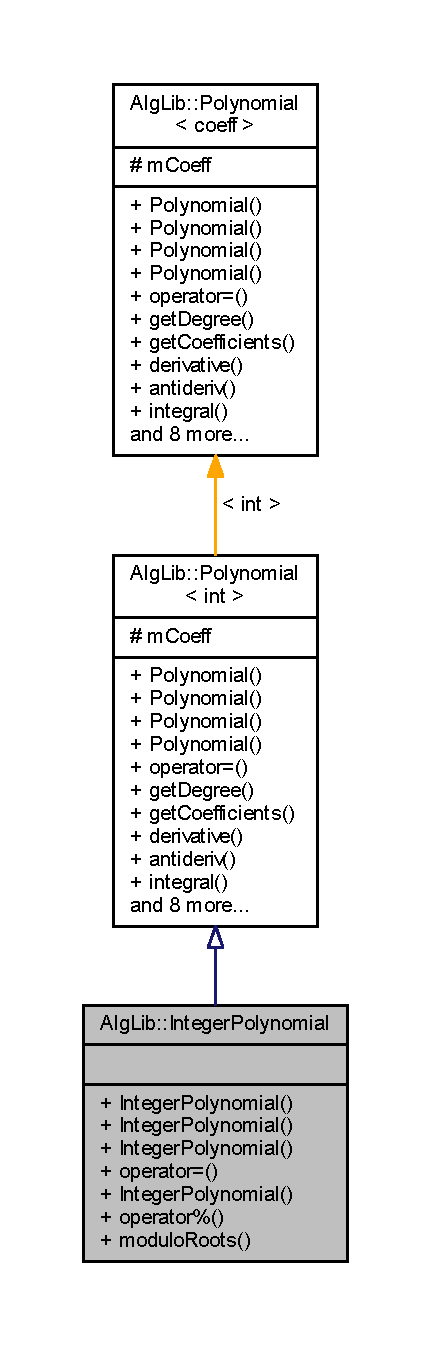
\includegraphics[height=550pt]{class_alg_lib_1_1_integer_polynomial__inherit__graph}
\end{center}
\end{figure}


Collaboration diagram for Alg\+Lib\+:\+:Integer\+Polynomial\+:\nopagebreak
\begin{figure}[H]
\begin{center}
\leavevmode
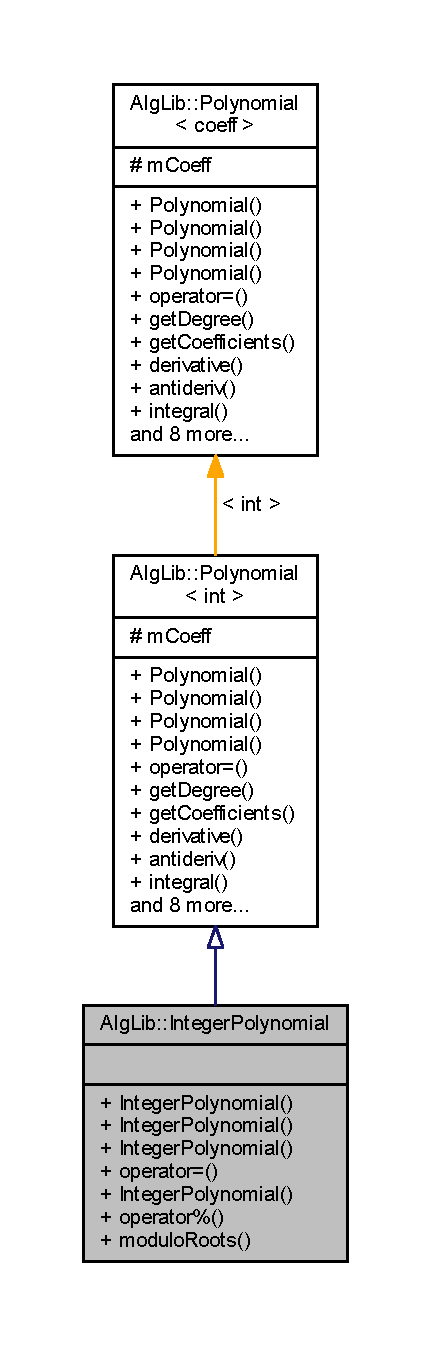
\includegraphics[height=550pt]{class_alg_lib_1_1_integer_polynomial__coll__graph}
\end{center}
\end{figure}
\subsection*{Public Member Functions}
\begin{DoxyCompactItemize}
\item 
\hyperlink{class_alg_lib_1_1_integer_polynomial_a655e9a0c3787323872d78194fb4321da}{Integer\+Polynomial} (std\+::vector$<$ int $>$ \&coefficients)
\begin{DoxyCompactList}\small\item\em (one liner) \end{DoxyCompactList}\item 
\hyperlink{class_alg_lib_1_1_integer_polynomial_a61873b5d4a577020238163251566077e}{Integer\+Polynomial} (std\+::initializer\+\_\+list$<$ int $>$ args)
\item 
\hyperlink{class_alg_lib_1_1_integer_polynomial_ae2f5396eab8162b3550db51bbcb30c55}{Integer\+Polynomial} (const \hyperlink{class_alg_lib_1_1_polynomial}{Polynomial}$<$ int $>$ \&other)
\item 
\hyperlink{class_alg_lib_1_1_integer_polynomial}{Integer\+Polynomial} \& \hyperlink{class_alg_lib_1_1_integer_polynomial_a6ce9a26baa35c33c35b91be4a930cf95}{operator=} (const \hyperlink{class_alg_lib_1_1_polynomial}{Polynomial}$<$ int $>$ \&other)
\item 
\hyperlink{class_alg_lib_1_1_integer_polynomial_ae74ad4d007e847f6bb385b93865bb88a}{Integer\+Polynomial} ()
\item 
virtual \hyperlink{class_alg_lib_1_1_integer_polynomial}{Integer\+Polynomial} \hyperlink{class_alg_lib_1_1_integer_polynomial_a2589da92ddd64bb3d2b52b7dbd197c07}{operator\%} (int mod) const 
\begin{DoxyCompactList}\small\item\em Takes modulo something. \end{DoxyCompactList}\item 
virtual std\+::vector$<$ int $>$ \hyperlink{class_alg_lib_1_1_integer_polynomial_ab0549a5f249b0b1c2868a784cd9b890b}{modulo\+Roots} (int mod) const 
\end{DoxyCompactItemize}
\subsection*{Additional Inherited Members}


\subsection{Detailed Description}


Definition at line 50 of file Polynomial.\+h.



\subsection{Constructor \& Destructor Documentation}
\index{Alg\+Lib\+::\+Integer\+Polynomial@{Alg\+Lib\+::\+Integer\+Polynomial}!Integer\+Polynomial@{Integer\+Polynomial}}
\index{Integer\+Polynomial@{Integer\+Polynomial}!Alg\+Lib\+::\+Integer\+Polynomial@{Alg\+Lib\+::\+Integer\+Polynomial}}
\subsubsection[{\texorpdfstring{Integer\+Polynomial(std\+::vector$<$ int $>$ \&coefficients)}{IntegerPolynomial(std::vector< int > &coefficients)}}]{\setlength{\rightskip}{0pt plus 5cm}Alg\+Lib\+::\+Integer\+Polynomial\+::\+Integer\+Polynomial (
\begin{DoxyParamCaption}
\item[{std\+::vector$<$ int $>$ \&}]{coefficients}
\end{DoxyParamCaption}
)}\hypertarget{class_alg_lib_1_1_integer_polynomial_a655e9a0c3787323872d78194fb4321da}{}\label{class_alg_lib_1_1_integer_polynomial_a655e9a0c3787323872d78194fb4321da}


(one liner) 

(documentation goes here) 

Definition at line 22 of file Int\+Polynomial.\+cpp.

\index{Alg\+Lib\+::\+Integer\+Polynomial@{Alg\+Lib\+::\+Integer\+Polynomial}!Integer\+Polynomial@{Integer\+Polynomial}}
\index{Integer\+Polynomial@{Integer\+Polynomial}!Alg\+Lib\+::\+Integer\+Polynomial@{Alg\+Lib\+::\+Integer\+Polynomial}}
\subsubsection[{\texorpdfstring{Integer\+Polynomial(std\+::initializer\+\_\+list$<$ int $>$ args)}{IntegerPolynomial(std::initializer_list< int > args)}}]{\setlength{\rightskip}{0pt plus 5cm}Alg\+Lib\+::\+Integer\+Polynomial\+::\+Integer\+Polynomial (
\begin{DoxyParamCaption}
\item[{std\+::initializer\+\_\+list$<$ int $>$}]{args}
\end{DoxyParamCaption}
)}\hypertarget{class_alg_lib_1_1_integer_polynomial_a61873b5d4a577020238163251566077e}{}\label{class_alg_lib_1_1_integer_polynomial_a61873b5d4a577020238163251566077e}


Definition at line 35 of file Int\+Polynomial.\+cpp.

\index{Alg\+Lib\+::\+Integer\+Polynomial@{Alg\+Lib\+::\+Integer\+Polynomial}!Integer\+Polynomial@{Integer\+Polynomial}}
\index{Integer\+Polynomial@{Integer\+Polynomial}!Alg\+Lib\+::\+Integer\+Polynomial@{Alg\+Lib\+::\+Integer\+Polynomial}}
\subsubsection[{\texorpdfstring{Integer\+Polynomial(const Polynomial$<$ int $>$ \&other)}{IntegerPolynomial(const Polynomial< int > &other)}}]{\setlength{\rightskip}{0pt plus 5cm}Alg\+Lib\+::\+Integer\+Polynomial\+::\+Integer\+Polynomial (
\begin{DoxyParamCaption}
\item[{const {\bf Polynomial}$<$ int $>$ \&}]{other}
\end{DoxyParamCaption}
)}\hypertarget{class_alg_lib_1_1_integer_polynomial_ae2f5396eab8162b3550db51bbcb30c55}{}\label{class_alg_lib_1_1_integer_polynomial_ae2f5396eab8162b3550db51bbcb30c55}


Definition at line 31 of file Int\+Polynomial.\+cpp.

\index{Alg\+Lib\+::\+Integer\+Polynomial@{Alg\+Lib\+::\+Integer\+Polynomial}!Integer\+Polynomial@{Integer\+Polynomial}}
\index{Integer\+Polynomial@{Integer\+Polynomial}!Alg\+Lib\+::\+Integer\+Polynomial@{Alg\+Lib\+::\+Integer\+Polynomial}}
\subsubsection[{\texorpdfstring{Integer\+Polynomial()}{IntegerPolynomial()}}]{\setlength{\rightskip}{0pt plus 5cm}Alg\+Lib\+::\+Integer\+Polynomial\+::\+Integer\+Polynomial (
\begin{DoxyParamCaption}
{}
\end{DoxyParamCaption}
)}\hypertarget{class_alg_lib_1_1_integer_polynomial_ae74ad4d007e847f6bb385b93865bb88a}{}\label{class_alg_lib_1_1_integer_polynomial_ae74ad4d007e847f6bb385b93865bb88a}


Definition at line 39 of file Int\+Polynomial.\+cpp.



\subsection{Member Function Documentation}
\index{Alg\+Lib\+::\+Integer\+Polynomial@{Alg\+Lib\+::\+Integer\+Polynomial}!modulo\+Roots@{modulo\+Roots}}
\index{modulo\+Roots@{modulo\+Roots}!Alg\+Lib\+::\+Integer\+Polynomial@{Alg\+Lib\+::\+Integer\+Polynomial}}
\subsubsection[{\texorpdfstring{modulo\+Roots(int mod) const }{moduloRoots(int mod) const }}]{\setlength{\rightskip}{0pt plus 5cm}std\+::vector$<$ int $>$ Alg\+Lib\+::\+Integer\+Polynomial\+::modulo\+Roots (
\begin{DoxyParamCaption}
\item[{int}]{mod}
\end{DoxyParamCaption}
) const\hspace{0.3cm}{\ttfamily [virtual]}}\hypertarget{class_alg_lib_1_1_integer_polynomial_ab0549a5f249b0b1c2868a784cd9b890b}{}\label{class_alg_lib_1_1_integer_polynomial_ab0549a5f249b0b1c2868a784cd9b890b}


Definition at line 44 of file Int\+Polynomial.\+cpp.

\index{Alg\+Lib\+::\+Integer\+Polynomial@{Alg\+Lib\+::\+Integer\+Polynomial}!operator\%@{operator\%}}
\index{operator\%@{operator\%}!Alg\+Lib\+::\+Integer\+Polynomial@{Alg\+Lib\+::\+Integer\+Polynomial}}
\subsubsection[{\texorpdfstring{operator\%(int mod) const }{operator%(int mod) const }}]{\setlength{\rightskip}{0pt plus 5cm}{\bf Alg\+Lib\+::\+Integer\+Polynomial} Alg\+Lib\+::\+Integer\+Polynomial\+::operator\% (
\begin{DoxyParamCaption}
\item[{int}]{mod}
\end{DoxyParamCaption}
) const\hspace{0.3cm}{\ttfamily [virtual]}}\hypertarget{class_alg_lib_1_1_integer_polynomial_a2589da92ddd64bb3d2b52b7dbd197c07}{}\label{class_alg_lib_1_1_integer_polynomial_a2589da92ddd64bb3d2b52b7dbd197c07}


Takes modulo something. 

Return \hyperlink{class_alg_lib_1_1_polynomial}{Polynomial} that takes the mod of the coefficients 

Definition at line 8 of file Int\+Polynomial.\+cpp.

\index{Alg\+Lib\+::\+Integer\+Polynomial@{Alg\+Lib\+::\+Integer\+Polynomial}!operator=@{operator=}}
\index{operator=@{operator=}!Alg\+Lib\+::\+Integer\+Polynomial@{Alg\+Lib\+::\+Integer\+Polynomial}}
\subsubsection[{\texorpdfstring{operator=(const Polynomial$<$ int $>$ \&other)}{operator=(const Polynomial< int > &other)}}]{\setlength{\rightskip}{0pt plus 5cm}{\bf Alg\+Lib\+::\+Integer\+Polynomial} \& Alg\+Lib\+::\+Integer\+Polynomial\+::operator= (
\begin{DoxyParamCaption}
\item[{const {\bf Polynomial}$<$ int $>$ \&}]{other}
\end{DoxyParamCaption}
)}\hypertarget{class_alg_lib_1_1_integer_polynomial_a6ce9a26baa35c33c35b91be4a930cf95}{}\label{class_alg_lib_1_1_integer_polynomial_a6ce9a26baa35c33c35b91be4a930cf95}


Definition at line 26 of file Int\+Polynomial.\+cpp.



The documentation for this class was generated from the following files\+:\begin{DoxyCompactItemize}
\item 
D\+:/\+Data/\+Desktop/\+Github/include/\hyperlink{_polynomial_8h}{Polynomial.\+h}\item 
D\+:/\+Data/\+Desktop/\+Github/src/\+Polynomial/\hyperlink{_int_polynomial_8cpp}{Int\+Polynomial.\+cpp}\end{DoxyCompactItemize}

\hypertarget{class_alg_lib_1_1_matrix}{}\section{Alg\+Lib\+:\+:Matrix$<$ T $>$ Class Template Reference}
\label{class_alg_lib_1_1_matrix}\index{Alg\+Lib\+::\+Matrix$<$ T $>$@{Alg\+Lib\+::\+Matrix$<$ T $>$}}


{\ttfamily \#include $<$Matrix.\+h$>$}



Inheritance diagram for Alg\+Lib\+:\+:Matrix$<$ T $>$\+:\nopagebreak
\begin{figure}[H]
\begin{center}
\leavevmode
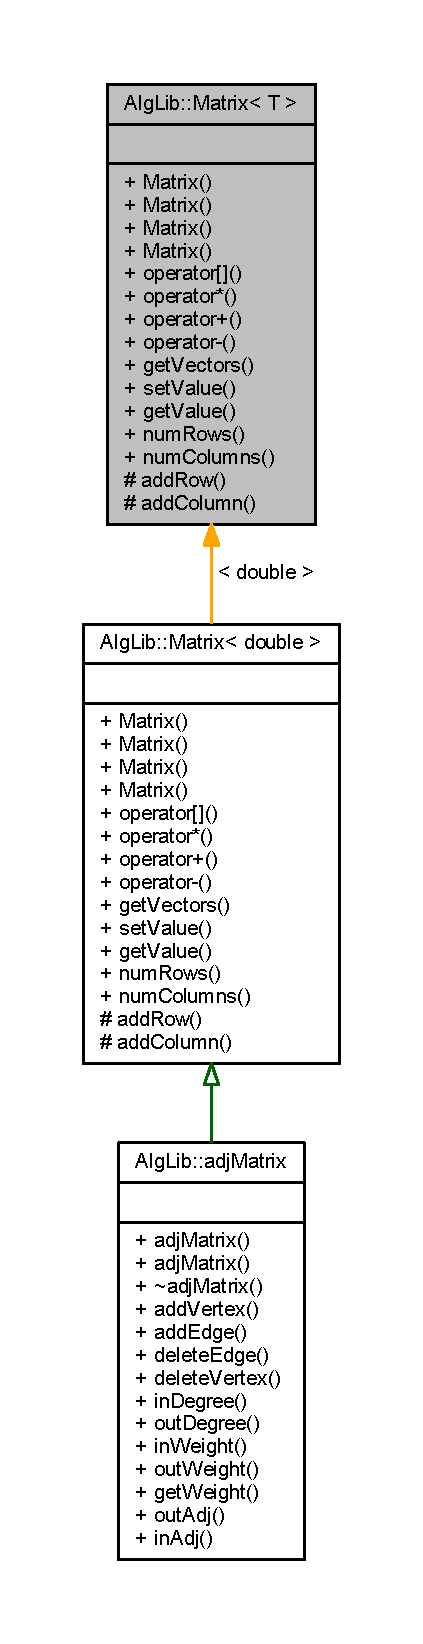
\includegraphics[height=550pt]{class_alg_lib_1_1_matrix__inherit__graph}
\end{center}
\end{figure}


Collaboration diagram for Alg\+Lib\+:\+:Matrix$<$ T $>$\+:\nopagebreak
\begin{figure}[H]
\begin{center}
\leavevmode
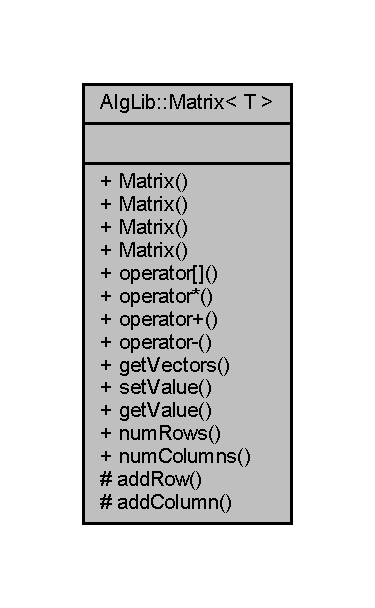
\includegraphics[width=180pt]{class_alg_lib_1_1_matrix__coll__graph}
\end{center}
\end{figure}
\subsection*{Public Member Functions}
\begin{DoxyCompactItemize}
\item 
\hyperlink{class_alg_lib_1_1_matrix_aa928f1b4f97f3689739fb76f37ea8b32}{Matrix} (int row, int column)
\item 
\hyperlink{class_alg_lib_1_1_matrix_ae5fe940d778538e4e9b92e559d4892f9}{Matrix} (const std\+::vector$<$ std\+::vector$<$ T $>$ $>$ \&the\+Matrix)
\item 
\hyperlink{class_alg_lib_1_1_matrix_a3c8f9c4d2a7a1d6235e364081c7b2291}{Matrix} (std\+::initializer\+\_\+list$<$ std\+::initializer\+\_\+list$<$ T $>$ $>$ m)
\item 
\hyperlink{class_alg_lib_1_1_matrix_af032730ee4314ca530b7926441135377}{Matrix} (const \hyperlink{class_alg_lib_1_1_matrix}{Matrix} \&rhs)
\item 
virtual std\+::vector$<$ T $>$ \& \hyperlink{class_alg_lib_1_1_matrix_aad964932a50c21c7b6f49f5193f42b3c}{operator\mbox{[}$\,$\mbox{]}} (int row)
\item 
virtual \hyperlink{class_alg_lib_1_1_matrix}{Matrix} \hyperlink{class_alg_lib_1_1_matrix_abd934caac0e4025576d38f2b9ebc85d0}{operator$\ast$} (const \hyperlink{class_alg_lib_1_1_matrix}{Matrix} \&other) const 
\item 
virtual \hyperlink{class_alg_lib_1_1_matrix}{Matrix} \hyperlink{class_alg_lib_1_1_matrix_ac85ab14586f80045033981c7751fd124}{operator+} (const \hyperlink{class_alg_lib_1_1_matrix}{Matrix} \&other) const 
\item 
virtual \hyperlink{class_alg_lib_1_1_matrix}{Matrix} \hyperlink{class_alg_lib_1_1_matrix_ae947b17fc992a714c6fc5dfa7365deb8}{operator-\/} (const \hyperlink{class_alg_lib_1_1_matrix}{Matrix} \&other) const 
\item 
virtual std\+::vector$<$ std\+::vector$<$ T $>$ $>$ \hyperlink{class_alg_lib_1_1_matrix_a5c651bc81f24c02ccbee007f4be49dfa}{get\+Vectors} () const 
\item 
virtual void \hyperlink{class_alg_lib_1_1_matrix_a434ac30c8fe0674d740ab8e513318cae}{set\+Value} (int row, int col, T value)
\item 
virtual T \hyperlink{class_alg_lib_1_1_matrix_a99342d63d4ed38c0289f14566381958e}{get\+Value} (int row, int col) const 
\item 
virtual int \hyperlink{class_alg_lib_1_1_matrix_ae78e1e7470110c5d8e43fe1199c6540e}{num\+Rows} () const 
\item 
virtual int \hyperlink{class_alg_lib_1_1_matrix_ac9a4892052b6d988fc79390528122f00}{num\+Columns} () const 
\end{DoxyCompactItemize}
\subsection*{Protected Member Functions}
\begin{DoxyCompactItemize}
\item 
virtual void \hyperlink{class_alg_lib_1_1_matrix_acb50a61a0a93f26ad60829edef419a3a}{add\+Row} ()
\item 
virtual void \hyperlink{class_alg_lib_1_1_matrix_a960028989285032b7c5847235358f894}{add\+Column} ()
\end{DoxyCompactItemize}


\subsection{Detailed Description}
\subsubsection*{template$<$typename T$>$\\*
class Alg\+Lib\+::\+Matrix$<$ T $>$}



Definition at line 11 of file Matrix.\+h.



\subsection{Constructor \& Destructor Documentation}
\index{Alg\+Lib\+::\+Matrix@{Alg\+Lib\+::\+Matrix}!Matrix@{Matrix}}
\index{Matrix@{Matrix}!Alg\+Lib\+::\+Matrix@{Alg\+Lib\+::\+Matrix}}
\subsubsection[{\texorpdfstring{Matrix(int row, int column)}{Matrix(int row, int column)}}]{\setlength{\rightskip}{0pt plus 5cm}template$<$typename T $>$ {\bf Alg\+Lib\+::\+Matrix}$<$ T $>$\+::{\bf Matrix} (
\begin{DoxyParamCaption}
\item[{int}]{row, }
\item[{int}]{column}
\end{DoxyParamCaption}
)}\hypertarget{class_alg_lib_1_1_matrix_aa928f1b4f97f3689739fb76f37ea8b32}{}\label{class_alg_lib_1_1_matrix_aa928f1b4f97f3689739fb76f37ea8b32}


Definition at line 7 of file Matrix.\+cpp.

\index{Alg\+Lib\+::\+Matrix@{Alg\+Lib\+::\+Matrix}!Matrix@{Matrix}}
\index{Matrix@{Matrix}!Alg\+Lib\+::\+Matrix@{Alg\+Lib\+::\+Matrix}}
\subsubsection[{\texorpdfstring{Matrix(const std\+::vector$<$ std\+::vector$<$ T $>$ $>$ \&the\+Matrix)}{Matrix(const std::vector< std::vector< T > > &theMatrix)}}]{\setlength{\rightskip}{0pt plus 5cm}template$<$typename T$>$ {\bf Alg\+Lib\+::\+Matrix}$<$ T $>$\+::{\bf Matrix} (
\begin{DoxyParamCaption}
\item[{const std\+::vector$<$ std\+::vector$<$ T $>$ $>$ \&}]{the\+Matrix}
\end{DoxyParamCaption}
)}\hypertarget{class_alg_lib_1_1_matrix_ae5fe940d778538e4e9b92e559d4892f9}{}\label{class_alg_lib_1_1_matrix_ae5fe940d778538e4e9b92e559d4892f9}


Definition at line 22 of file Matrix.\+cpp.

\index{Alg\+Lib\+::\+Matrix@{Alg\+Lib\+::\+Matrix}!Matrix@{Matrix}}
\index{Matrix@{Matrix}!Alg\+Lib\+::\+Matrix@{Alg\+Lib\+::\+Matrix}}
\subsubsection[{\texorpdfstring{Matrix(std\+::initializer\+\_\+list$<$ std\+::initializer\+\_\+list$<$ T $>$ $>$ m)}{Matrix(std::initializer_list< std::initializer_list< T > > m)}}]{\setlength{\rightskip}{0pt plus 5cm}template$<$typename T$>$ {\bf Alg\+Lib\+::\+Matrix}$<$ T $>$\+::{\bf Matrix} (
\begin{DoxyParamCaption}
\item[{std\+::initializer\+\_\+list$<$ std\+::initializer\+\_\+list$<$ T $>$ $>$}]{m}
\end{DoxyParamCaption}
)}\hypertarget{class_alg_lib_1_1_matrix_a3c8f9c4d2a7a1d6235e364081c7b2291}{}\label{class_alg_lib_1_1_matrix_a3c8f9c4d2a7a1d6235e364081c7b2291}


Definition at line 33 of file Matrix.\+cpp.

\index{Alg\+Lib\+::\+Matrix@{Alg\+Lib\+::\+Matrix}!Matrix@{Matrix}}
\index{Matrix@{Matrix}!Alg\+Lib\+::\+Matrix@{Alg\+Lib\+::\+Matrix}}
\subsubsection[{\texorpdfstring{Matrix(const Matrix \&rhs)}{Matrix(const Matrix &rhs)}}]{\setlength{\rightskip}{0pt plus 5cm}template$<$typename T$>$ {\bf Alg\+Lib\+::\+Matrix}$<$ T $>$\+::{\bf Matrix} (
\begin{DoxyParamCaption}
\item[{const {\bf Matrix}$<$ T $>$ \&}]{rhs}
\end{DoxyParamCaption}
)}\hypertarget{class_alg_lib_1_1_matrix_af032730ee4314ca530b7926441135377}{}\label{class_alg_lib_1_1_matrix_af032730ee4314ca530b7926441135377}
Copy constructor 

Definition at line 59 of file Matrix.\+cpp.



\subsection{Member Function Documentation}
\index{Alg\+Lib\+::\+Matrix@{Alg\+Lib\+::\+Matrix}!add\+Column@{add\+Column}}
\index{add\+Column@{add\+Column}!Alg\+Lib\+::\+Matrix@{Alg\+Lib\+::\+Matrix}}
\subsubsection[{\texorpdfstring{add\+Column()}{addColumn()}}]{\setlength{\rightskip}{0pt plus 5cm}template$<$typename T $>$ void {\bf Alg\+Lib\+::\+Matrix}$<$ T $>$\+::add\+Column (
\begin{DoxyParamCaption}
{}
\end{DoxyParamCaption}
)\hspace{0.3cm}{\ttfamily [protected]}, {\ttfamily [virtual]}}\hypertarget{class_alg_lib_1_1_matrix_a960028989285032b7c5847235358f894}{}\label{class_alg_lib_1_1_matrix_a960028989285032b7c5847235358f894}


Definition at line 176 of file Matrix.\+cpp.

\index{Alg\+Lib\+::\+Matrix@{Alg\+Lib\+::\+Matrix}!add\+Row@{add\+Row}}
\index{add\+Row@{add\+Row}!Alg\+Lib\+::\+Matrix@{Alg\+Lib\+::\+Matrix}}
\subsubsection[{\texorpdfstring{add\+Row()}{addRow()}}]{\setlength{\rightskip}{0pt plus 5cm}template$<$typename T $>$ void {\bf Alg\+Lib\+::\+Matrix}$<$ T $>$\+::add\+Row (
\begin{DoxyParamCaption}
{}
\end{DoxyParamCaption}
)\hspace{0.3cm}{\ttfamily [protected]}, {\ttfamily [virtual]}}\hypertarget{class_alg_lib_1_1_matrix_acb50a61a0a93f26ad60829edef419a3a}{}\label{class_alg_lib_1_1_matrix_acb50a61a0a93f26ad60829edef419a3a}


Definition at line 170 of file Matrix.\+cpp.

\index{Alg\+Lib\+::\+Matrix@{Alg\+Lib\+::\+Matrix}!get\+Value@{get\+Value}}
\index{get\+Value@{get\+Value}!Alg\+Lib\+::\+Matrix@{Alg\+Lib\+::\+Matrix}}
\subsubsection[{\texorpdfstring{get\+Value(int row, int col) const }{getValue(int row, int col) const }}]{\setlength{\rightskip}{0pt plus 5cm}template$<$typename T $>$ T {\bf Alg\+Lib\+::\+Matrix}$<$ T $>$\+::get\+Value (
\begin{DoxyParamCaption}
\item[{int}]{row, }
\item[{int}]{col}
\end{DoxyParamCaption}
) const\hspace{0.3cm}{\ttfamily [virtual]}}\hypertarget{class_alg_lib_1_1_matrix_a99342d63d4ed38c0289f14566381958e}{}\label{class_alg_lib_1_1_matrix_a99342d63d4ed38c0289f14566381958e}


Definition at line 185 of file Matrix.\+cpp.

\index{Alg\+Lib\+::\+Matrix@{Alg\+Lib\+::\+Matrix}!get\+Vectors@{get\+Vectors}}
\index{get\+Vectors@{get\+Vectors}!Alg\+Lib\+::\+Matrix@{Alg\+Lib\+::\+Matrix}}
\subsubsection[{\texorpdfstring{get\+Vectors() const }{getVectors() const }}]{\setlength{\rightskip}{0pt plus 5cm}template$<$typename T $>$ std\+::vector$<$ std\+::vector$<$ T $>$ $>$ {\bf Alg\+Lib\+::\+Matrix}$<$ T $>$\+::get\+Vectors (
\begin{DoxyParamCaption}
{}
\end{DoxyParamCaption}
) const\hspace{0.3cm}{\ttfamily [virtual]}}\hypertarget{class_alg_lib_1_1_matrix_a5c651bc81f24c02ccbee007f4be49dfa}{}\label{class_alg_lib_1_1_matrix_a5c651bc81f24c02ccbee007f4be49dfa}


Definition at line 79 of file Matrix.\+cpp.

\index{Alg\+Lib\+::\+Matrix@{Alg\+Lib\+::\+Matrix}!num\+Columns@{num\+Columns}}
\index{num\+Columns@{num\+Columns}!Alg\+Lib\+::\+Matrix@{Alg\+Lib\+::\+Matrix}}
\subsubsection[{\texorpdfstring{num\+Columns() const }{numColumns() const }}]{\setlength{\rightskip}{0pt plus 5cm}template$<$typename T $>$ int {\bf Alg\+Lib\+::\+Matrix}$<$ T $>$\+::num\+Columns (
\begin{DoxyParamCaption}
{}
\end{DoxyParamCaption}
) const\hspace{0.3cm}{\ttfamily [virtual]}}\hypertarget{class_alg_lib_1_1_matrix_ac9a4892052b6d988fc79390528122f00}{}\label{class_alg_lib_1_1_matrix_ac9a4892052b6d988fc79390528122f00}


Definition at line 164 of file Matrix.\+cpp.

\index{Alg\+Lib\+::\+Matrix@{Alg\+Lib\+::\+Matrix}!num\+Rows@{num\+Rows}}
\index{num\+Rows@{num\+Rows}!Alg\+Lib\+::\+Matrix@{Alg\+Lib\+::\+Matrix}}
\subsubsection[{\texorpdfstring{num\+Rows() const }{numRows() const }}]{\setlength{\rightskip}{0pt plus 5cm}template$<$typename T $>$ int {\bf Alg\+Lib\+::\+Matrix}$<$ T $>$\+::num\+Rows (
\begin{DoxyParamCaption}
{}
\end{DoxyParamCaption}
) const\hspace{0.3cm}{\ttfamily [virtual]}}\hypertarget{class_alg_lib_1_1_matrix_ae78e1e7470110c5d8e43fe1199c6540e}{}\label{class_alg_lib_1_1_matrix_ae78e1e7470110c5d8e43fe1199c6540e}


Definition at line 159 of file Matrix.\+cpp.

\index{Alg\+Lib\+::\+Matrix@{Alg\+Lib\+::\+Matrix}!operator$\ast$@{operator$\ast$}}
\index{operator$\ast$@{operator$\ast$}!Alg\+Lib\+::\+Matrix@{Alg\+Lib\+::\+Matrix}}
\subsubsection[{\texorpdfstring{operator$\ast$(const Matrix \&other) const }{operator*(const Matrix &other) const }}]{\setlength{\rightskip}{0pt plus 5cm}template$<$typename T $>$ {\bf Matrix}$<$ T $>$ {\bf Alg\+Lib\+::\+Matrix}$<$ T $>$\+::operator$\ast$ (
\begin{DoxyParamCaption}
\item[{const {\bf Matrix}$<$ T $>$ \&}]{other}
\end{DoxyParamCaption}
) const\hspace{0.3cm}{\ttfamily [virtual]}}\hypertarget{class_alg_lib_1_1_matrix_abd934caac0e4025576d38f2b9ebc85d0}{}\label{class_alg_lib_1_1_matrix_abd934caac0e4025576d38f2b9ebc85d0}


Definition at line 137 of file Matrix.\+cpp.

\index{Alg\+Lib\+::\+Matrix@{Alg\+Lib\+::\+Matrix}!operator+@{operator+}}
\index{operator+@{operator+}!Alg\+Lib\+::\+Matrix@{Alg\+Lib\+::\+Matrix}}
\subsubsection[{\texorpdfstring{operator+(const Matrix \&other) const }{operator+(const Matrix &other) const }}]{\setlength{\rightskip}{0pt plus 5cm}template$<$typename T $>$ {\bf Matrix}$<$ T $>$ {\bf Alg\+Lib\+::\+Matrix}$<$ T $>$\+::operator+ (
\begin{DoxyParamCaption}
\item[{const {\bf Matrix}$<$ T $>$ \&}]{other}
\end{DoxyParamCaption}
) const\hspace{0.3cm}{\ttfamily [virtual]}}\hypertarget{class_alg_lib_1_1_matrix_ac85ab14586f80045033981c7751fd124}{}\label{class_alg_lib_1_1_matrix_ac85ab14586f80045033981c7751fd124}


Definition at line 99 of file Matrix.\+cpp.

\index{Alg\+Lib\+::\+Matrix@{Alg\+Lib\+::\+Matrix}!operator-\/@{operator-\/}}
\index{operator-\/@{operator-\/}!Alg\+Lib\+::\+Matrix@{Alg\+Lib\+::\+Matrix}}
\subsubsection[{\texorpdfstring{operator-\/(const Matrix \&other) const }{operator-(const Matrix &other) const }}]{\setlength{\rightskip}{0pt plus 5cm}template$<$typename T $>$ {\bf Matrix}$<$ T $>$ {\bf Alg\+Lib\+::\+Matrix}$<$ T $>$\+::operator-\/ (
\begin{DoxyParamCaption}
\item[{const {\bf Matrix}$<$ T $>$ \&}]{other}
\end{DoxyParamCaption}
) const\hspace{0.3cm}{\ttfamily [virtual]}}\hypertarget{class_alg_lib_1_1_matrix_ae947b17fc992a714c6fc5dfa7365deb8}{}\label{class_alg_lib_1_1_matrix_ae947b17fc992a714c6fc5dfa7365deb8}


Definition at line 118 of file Matrix.\+cpp.

\index{Alg\+Lib\+::\+Matrix@{Alg\+Lib\+::\+Matrix}!operator\mbox{[}$\,$\mbox{]}@{operator[]}}
\index{operator\mbox{[}$\,$\mbox{]}@{operator[]}!Alg\+Lib\+::\+Matrix@{Alg\+Lib\+::\+Matrix}}
\subsubsection[{\texorpdfstring{operator[](int row)}{operator[](int row)}}]{\setlength{\rightskip}{0pt plus 5cm}template$<$typename T $>$ std\+::vector$<$ T $>$ \& {\bf Alg\+Lib\+::\+Matrix}$<$ T $>$\+::operator\mbox{[}$\,$\mbox{]} (
\begin{DoxyParamCaption}
\item[{int}]{row}
\end{DoxyParamCaption}
)\hspace{0.3cm}{\ttfamily [virtual]}}\hypertarget{class_alg_lib_1_1_matrix_aad964932a50c21c7b6f49f5193f42b3c}{}\label{class_alg_lib_1_1_matrix_aad964932a50c21c7b6f49f5193f42b3c}


Definition at line 93 of file Matrix.\+cpp.

\index{Alg\+Lib\+::\+Matrix@{Alg\+Lib\+::\+Matrix}!set\+Value@{set\+Value}}
\index{set\+Value@{set\+Value}!Alg\+Lib\+::\+Matrix@{Alg\+Lib\+::\+Matrix}}
\subsubsection[{\texorpdfstring{set\+Value(int row, int col, T value)}{setValue(int row, int col, T value)}}]{\setlength{\rightskip}{0pt plus 5cm}template$<$typename T$>$ void {\bf Alg\+Lib\+::\+Matrix}$<$ T $>$\+::set\+Value (
\begin{DoxyParamCaption}
\item[{int}]{row, }
\item[{int}]{col, }
\item[{T}]{value}
\end{DoxyParamCaption}
)\hspace{0.3cm}{\ttfamily [virtual]}}\hypertarget{class_alg_lib_1_1_matrix_a434ac30c8fe0674d740ab8e513318cae}{}\label{class_alg_lib_1_1_matrix_a434ac30c8fe0674d740ab8e513318cae}


Definition at line 85 of file Matrix.\+cpp.



The documentation for this class was generated from the following files\+:\begin{DoxyCompactItemize}
\item 
D\+:/\+Data/\+Desktop/\+Github/include/\hyperlink{_matrix_8h}{Matrix.\+h}\item 
D\+:/\+Data/\+Desktop/\+Github/src/\+Matrix/\hyperlink{_matrix_8cpp}{Matrix.\+cpp}\end{DoxyCompactItemize}

\hypertarget{class_alg_lib_1_1_permutation}{}\section{Alg\+Lib\+:\+:Permutation$<$ T $>$ Class Template Reference}
\label{class_alg_lib_1_1_permutation}\index{Alg\+Lib\+::\+Permutation$<$ T $>$@{Alg\+Lib\+::\+Permutation$<$ T $>$}}


{\ttfamily \#include $<$Permutation.\+h$>$}



Collaboration diagram for Alg\+Lib\+:\+:Permutation$<$ T $>$\+:\nopagebreak
\begin{figure}[H]
\begin{center}
\leavevmode
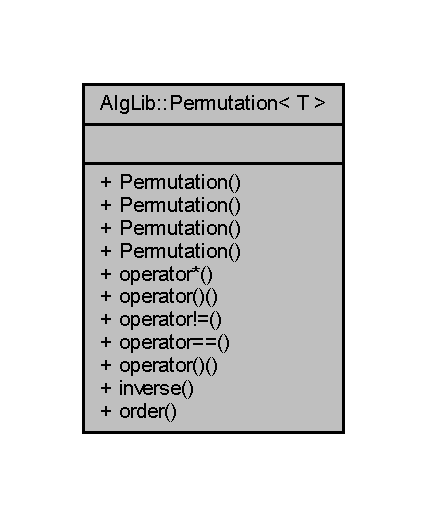
\includegraphics[width=205pt]{class_alg_lib_1_1_permutation__coll__graph}
\end{center}
\end{figure}
\subsection*{Public Member Functions}
\begin{DoxyCompactItemize}
\item 
\hyperlink{class_alg_lib_1_1_permutation_ae72beae52a1669396d13441b72709683}{Permutation} ()
\item 
\hyperlink{class_alg_lib_1_1_permutation_a1b2028a9b4cc2f593ee8037ae25e4ec8}{Permutation} (std\+::initializer\+\_\+list$<$ int $>$ word)
\item 
\hyperlink{class_alg_lib_1_1_permutation_a31e05184954e85e206b1ca6dc4dfe25f}{Permutation} (std\+::initializer\+\_\+list$<$ std\+::initializer\+\_\+list$<$ T $>$$>$ cycles)
\item 
\hyperlink{class_alg_lib_1_1_permutation_a6cea586e990533bc9c5dc649f28ca2e2}{Permutation} (std\+::vector$<$ std\+::pair$<$ T, T $>$$>$ pairs)
\item 
virtual \hyperlink{class_alg_lib_1_1_permutation}{Permutation}$<$ T $>$ \hyperlink{class_alg_lib_1_1_permutation_a495faf3699aa7996f19829816498efdb}{operator$\ast$} (const \hyperlink{class_alg_lib_1_1_permutation}{Permutation}$<$ T $>$ \&other) const 
\item 
virtual std\+::vector$<$ T $>$ \hyperlink{class_alg_lib_1_1_permutation_a1f773aa53b671a8f5930f50daffae15c}{operator()} (const std\+::vector$<$ T $>$ \&li) const 
\item 
virtual bool \hyperlink{class_alg_lib_1_1_permutation_a195d7015d44c650db9b7fec897b165a0}{operator!=} (const \hyperlink{class_alg_lib_1_1_permutation}{Permutation}$<$ T $>$ \&other) const 
\item 
virtual bool \hyperlink{class_alg_lib_1_1_permutation_a07235b740895334671099e3b02b6168f}{operator==} (const \hyperlink{class_alg_lib_1_1_permutation}{Permutation}$<$ T $>$ \&other) const 
\item 
virtual T \hyperlink{class_alg_lib_1_1_permutation_a6ecb0760c9ed48542b4a93a8b842bb0b}{operator()} (const T elem) const 
\item 
virtual \hyperlink{class_alg_lib_1_1_permutation}{Permutation}$<$ T $>$ \hyperlink{class_alg_lib_1_1_permutation_ac5f361e8a5cab1dbb331341e9d3c76b0}{inverse} ()
\item 
virtual int \hyperlink{class_alg_lib_1_1_permutation_a0241c0e6e52419e08832620e607caeba}{order} ()
\end{DoxyCompactItemize}


\subsection{Detailed Description}
\subsubsection*{template$<$typename T$>$\\*
class Alg\+Lib\+::\+Permutation$<$ T $>$}



Definition at line 12 of file Permutation.\+h.



\subsection{Constructor \& Destructor Documentation}
\index{Alg\+Lib\+::\+Permutation@{Alg\+Lib\+::\+Permutation}!Permutation@{Permutation}}
\index{Permutation@{Permutation}!Alg\+Lib\+::\+Permutation@{Alg\+Lib\+::\+Permutation}}
\subsubsection[{\texorpdfstring{Permutation()}{Permutation()}}]{\setlength{\rightskip}{0pt plus 5cm}template$<$typename T $>$ {\bf Alg\+Lib\+::\+Permutation}$<$ T $>$\+::{\bf Permutation} (
\begin{DoxyParamCaption}
{}
\end{DoxyParamCaption}
)}\hypertarget{class_alg_lib_1_1_permutation_ae72beae52a1669396d13441b72709683}{}\label{class_alg_lib_1_1_permutation_ae72beae52a1669396d13441b72709683}


Definition at line 13 of file Permutation.\+cpp.

\index{Alg\+Lib\+::\+Permutation@{Alg\+Lib\+::\+Permutation}!Permutation@{Permutation}}
\index{Permutation@{Permutation}!Alg\+Lib\+::\+Permutation@{Alg\+Lib\+::\+Permutation}}
\subsubsection[{\texorpdfstring{Permutation(std\+::initializer\+\_\+list$<$ int $>$ word)}{Permutation(std::initializer_list< int > word)}}]{\setlength{\rightskip}{0pt plus 5cm}template$<$typename T $>$ {\bf Alg\+Lib\+::\+Permutation}$<$ T $>$\+::{\bf Permutation} (
\begin{DoxyParamCaption}
\item[{std\+::initializer\+\_\+list$<$ int $>$}]{word}
\end{DoxyParamCaption}
)}\hypertarget{class_alg_lib_1_1_permutation_a1b2028a9b4cc2f593ee8037ae25e4ec8}{}\label{class_alg_lib_1_1_permutation_a1b2028a9b4cc2f593ee8037ae25e4ec8}


Definition at line 17 of file Permutation.\+cpp.

\index{Alg\+Lib\+::\+Permutation@{Alg\+Lib\+::\+Permutation}!Permutation@{Permutation}}
\index{Permutation@{Permutation}!Alg\+Lib\+::\+Permutation@{Alg\+Lib\+::\+Permutation}}
\subsubsection[{\texorpdfstring{Permutation(std\+::initializer\+\_\+list$<$ std\+::initializer\+\_\+list$<$ T $>$$>$ cycles)}{Permutation(std::initializer_list< std::initializer_list< T >> cycles)}}]{\setlength{\rightskip}{0pt plus 5cm}template$<$typename T $>$ {\bf Alg\+Lib\+::\+Permutation}$<$ T $>$\+::{\bf Permutation} (
\begin{DoxyParamCaption}
\item[{std\+::initializer\+\_\+list$<$ std\+::initializer\+\_\+list$<$ T $>$$>$}]{cycles}
\end{DoxyParamCaption}
)}\hypertarget{class_alg_lib_1_1_permutation_a31e05184954e85e206b1ca6dc4dfe25f}{}\label{class_alg_lib_1_1_permutation_a31e05184954e85e206b1ca6dc4dfe25f}


Definition at line 27 of file Permutation.\+cpp.

\index{Alg\+Lib\+::\+Permutation@{Alg\+Lib\+::\+Permutation}!Permutation@{Permutation}}
\index{Permutation@{Permutation}!Alg\+Lib\+::\+Permutation@{Alg\+Lib\+::\+Permutation}}
\subsubsection[{\texorpdfstring{Permutation(std\+::vector$<$ std\+::pair$<$ T, T $>$$>$ pairs)}{Permutation(std::vector< std::pair< T, T >> pairs)}}]{\setlength{\rightskip}{0pt plus 5cm}template$<$typename T $>$ {\bf Alg\+Lib\+::\+Permutation}$<$ T $>$\+::{\bf Permutation} (
\begin{DoxyParamCaption}
\item[{std\+::vector$<$ std\+::pair$<$ T, T $>$$>$}]{pairs}
\end{DoxyParamCaption}
)}\hypertarget{class_alg_lib_1_1_permutation_a6cea586e990533bc9c5dc649f28ca2e2}{}\label{class_alg_lib_1_1_permutation_a6cea586e990533bc9c5dc649f28ca2e2}


Definition at line 38 of file Permutation.\+cpp.



\subsection{Member Function Documentation}
\index{Alg\+Lib\+::\+Permutation@{Alg\+Lib\+::\+Permutation}!inverse@{inverse}}
\index{inverse@{inverse}!Alg\+Lib\+::\+Permutation@{Alg\+Lib\+::\+Permutation}}
\subsubsection[{\texorpdfstring{inverse()}{inverse()}}]{\setlength{\rightskip}{0pt plus 5cm}template$<$typename T $>$ {\bf Alg\+Lib\+::\+Permutation}$<$ T $>$ {\bf Alg\+Lib\+::\+Permutation}$<$ T $>$\+::inverse (
\begin{DoxyParamCaption}
{}
\end{DoxyParamCaption}
)\hspace{0.3cm}{\ttfamily [virtual]}}\hypertarget{class_alg_lib_1_1_permutation_ac5f361e8a5cab1dbb331341e9d3c76b0}{}\label{class_alg_lib_1_1_permutation_ac5f361e8a5cab1dbb331341e9d3c76b0}


Definition at line 75 of file Permutation.\+cpp.

\index{Alg\+Lib\+::\+Permutation@{Alg\+Lib\+::\+Permutation}!operator"!=@{operator"!=}}
\index{operator"!=@{operator"!=}!Alg\+Lib\+::\+Permutation@{Alg\+Lib\+::\+Permutation}}
\subsubsection[{\texorpdfstring{operator"!=(const Permutation$<$ T $>$ \&other) const }{operator!=(const Permutation< T > &other) const }}]{\setlength{\rightskip}{0pt plus 5cm}template$<$typename T $>$ bool {\bf Alg\+Lib\+::\+Permutation}$<$ T $>$\+::operator!= (
\begin{DoxyParamCaption}
\item[{const {\bf Permutation}$<$ T $>$ \&}]{other}
\end{DoxyParamCaption}
) const\hspace{0.3cm}{\ttfamily [virtual]}}\hypertarget{class_alg_lib_1_1_permutation_a195d7015d44c650db9b7fec897b165a0}{}\label{class_alg_lib_1_1_permutation_a195d7015d44c650db9b7fec897b165a0}


Definition at line 140 of file Permutation.\+cpp.

\index{Alg\+Lib\+::\+Permutation@{Alg\+Lib\+::\+Permutation}!operator()@{operator()}}
\index{operator()@{operator()}!Alg\+Lib\+::\+Permutation@{Alg\+Lib\+::\+Permutation}}
\subsubsection[{\texorpdfstring{operator()(const std\+::vector$<$ T $>$ \&li) const }{operator()(const std::vector< T > &li) const }}]{\setlength{\rightskip}{0pt plus 5cm}template$<$typename T $>$ std\+::vector$<$ T $>$ {\bf Alg\+Lib\+::\+Permutation}$<$ T $>$\+::operator() (
\begin{DoxyParamCaption}
\item[{const std\+::vector$<$ T $>$ \&}]{li}
\end{DoxyParamCaption}
) const\hspace{0.3cm}{\ttfamily [virtual]}}\hypertarget{class_alg_lib_1_1_permutation_a1f773aa53b671a8f5930f50daffae15c}{}\label{class_alg_lib_1_1_permutation_a1f773aa53b671a8f5930f50daffae15c}


Definition at line 46 of file Permutation.\+cpp.

\index{Alg\+Lib\+::\+Permutation@{Alg\+Lib\+::\+Permutation}!operator()@{operator()}}
\index{operator()@{operator()}!Alg\+Lib\+::\+Permutation@{Alg\+Lib\+::\+Permutation}}
\subsubsection[{\texorpdfstring{operator()(const T elem) const }{operator()(const T elem) const }}]{\setlength{\rightskip}{0pt plus 5cm}template$<$typename T $>$ T {\bf Alg\+Lib\+::\+Permutation}$<$ T $>$\+::operator() (
\begin{DoxyParamCaption}
\item[{const T}]{elem}
\end{DoxyParamCaption}
) const\hspace{0.3cm}{\ttfamily [virtual]}}\hypertarget{class_alg_lib_1_1_permutation_a6ecb0760c9ed48542b4a93a8b842bb0b}{}\label{class_alg_lib_1_1_permutation_a6ecb0760c9ed48542b4a93a8b842bb0b}


Definition at line 65 of file Permutation.\+cpp.

\index{Alg\+Lib\+::\+Permutation@{Alg\+Lib\+::\+Permutation}!operator$\ast$@{operator$\ast$}}
\index{operator$\ast$@{operator$\ast$}!Alg\+Lib\+::\+Permutation@{Alg\+Lib\+::\+Permutation}}
\subsubsection[{\texorpdfstring{operator$\ast$(const Permutation$<$ T $>$ \&other) const }{operator*(const Permutation< T > &other) const }}]{\setlength{\rightskip}{0pt plus 5cm}template$<$typename T $>$ {\bf Alg\+Lib\+::\+Permutation}$<$ T $>$ {\bf Alg\+Lib\+::\+Permutation}$<$ T $>$\+::operator$\ast$ (
\begin{DoxyParamCaption}
\item[{const {\bf Permutation}$<$ T $>$ \&}]{other}
\end{DoxyParamCaption}
) const\hspace{0.3cm}{\ttfamily [virtual]}}\hypertarget{class_alg_lib_1_1_permutation_a495faf3699aa7996f19829816498efdb}{}\label{class_alg_lib_1_1_permutation_a495faf3699aa7996f19829816498efdb}


Definition at line 85 of file Permutation.\+cpp.

\index{Alg\+Lib\+::\+Permutation@{Alg\+Lib\+::\+Permutation}!operator==@{operator==}}
\index{operator==@{operator==}!Alg\+Lib\+::\+Permutation@{Alg\+Lib\+::\+Permutation}}
\subsubsection[{\texorpdfstring{operator==(const Permutation$<$ T $>$ \&other) const }{operator==(const Permutation< T > &other) const }}]{\setlength{\rightskip}{0pt plus 5cm}template$<$typename T $>$ bool {\bf Alg\+Lib\+::\+Permutation}$<$ T $>$\+::operator== (
\begin{DoxyParamCaption}
\item[{const {\bf Permutation}$<$ T $>$ \&}]{other}
\end{DoxyParamCaption}
) const\hspace{0.3cm}{\ttfamily [virtual]}}\hypertarget{class_alg_lib_1_1_permutation_a07235b740895334671099e3b02b6168f}{}\label{class_alg_lib_1_1_permutation_a07235b740895334671099e3b02b6168f}


Definition at line 107 of file Permutation.\+cpp.

\index{Alg\+Lib\+::\+Permutation@{Alg\+Lib\+::\+Permutation}!order@{order}}
\index{order@{order}!Alg\+Lib\+::\+Permutation@{Alg\+Lib\+::\+Permutation}}
\subsubsection[{\texorpdfstring{order()}{order()}}]{\setlength{\rightskip}{0pt plus 5cm}template$<$typename T $>$ int {\bf Alg\+Lib\+::\+Permutation}$<$ T $>$\+::order (
\begin{DoxyParamCaption}
{}
\end{DoxyParamCaption}
)\hspace{0.3cm}{\ttfamily [virtual]}}\hypertarget{class_alg_lib_1_1_permutation_a0241c0e6e52419e08832620e607caeba}{}\label{class_alg_lib_1_1_permutation_a0241c0e6e52419e08832620e607caeba}


Definition at line 95 of file Permutation.\+cpp.



The documentation for this class was generated from the following files\+:\begin{DoxyCompactItemize}
\item 
D\+:/\+Data/\+Desktop/\+Github/include/\hyperlink{_permutation_8h}{Permutation.\+h}\item 
D\+:/\+Data/\+Desktop/\+Github/src/\+Permutation/\hyperlink{_permutation_8cpp}{Permutation.\+cpp}\end{DoxyCompactItemize}

\hypertarget{class_alg_lib_1_1_polynomial}{}\section{Alg\+Lib\+:\+:Polynomial$<$ coeff $>$ Class Template Reference}
\label{class_alg_lib_1_1_polynomial}\index{Alg\+Lib\+::\+Polynomial$<$ coeff $>$@{Alg\+Lib\+::\+Polynomial$<$ coeff $>$}}


{\ttfamily \#include $<$Polynomial.\+h$>$}



Inheritance diagram for Alg\+Lib\+:\+:Polynomial$<$ coeff $>$\+:\nopagebreak
\begin{figure}[H]
\begin{center}
\leavevmode
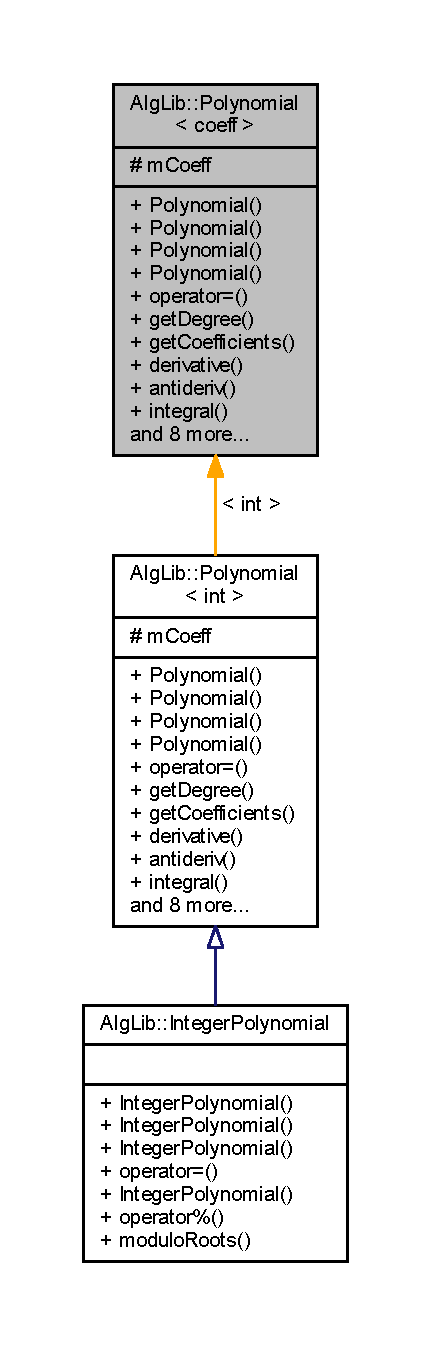
\includegraphics[height=550pt]{class_alg_lib_1_1_polynomial__inherit__graph}
\end{center}
\end{figure}


Collaboration diagram for Alg\+Lib\+:\+:Polynomial$<$ coeff $>$\+:\nopagebreak
\begin{figure}[H]
\begin{center}
\leavevmode
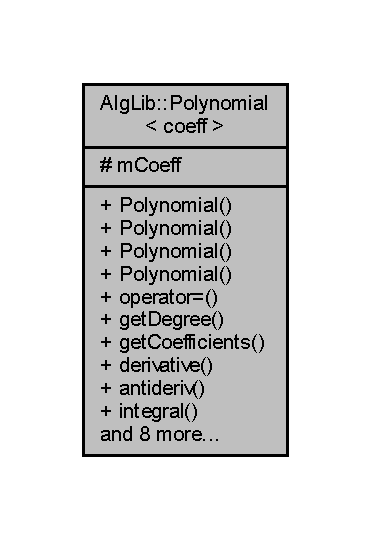
\includegraphics[width=178pt]{class_alg_lib_1_1_polynomial__coll__graph}
\end{center}
\end{figure}
\subsection*{Public Member Functions}
\begin{DoxyCompactItemize}
\item 
\hyperlink{class_alg_lib_1_1_polynomial_a33a0ad0b646bcf6b0295d597097fed85}{Polynomial} ()
\item 
\hyperlink{class_alg_lib_1_1_polynomial_a53075cc00bf37bcaf2ff6c8d18ec3206}{Polynomial} (std\+::initializer\+\_\+list$<$ coeff $>$ args)
\item 
\hyperlink{class_alg_lib_1_1_polynomial_ad75097bb323e32318e6b508532ebce7a}{Polynomial} (std\+::vector$<$ coeff $>$ coefficients)
\item 
\hyperlink{class_alg_lib_1_1_polynomial_af16630d7204b1bb4f4353682a851abdb}{Polynomial} (const \hyperlink{class_alg_lib_1_1_polynomial}{Polynomial}$<$ coeff $>$ \&rhs)
\item 
\hyperlink{class_alg_lib_1_1_polynomial}{Polynomial} \& \hyperlink{class_alg_lib_1_1_polynomial_adb6aa23b16a21e65973e771c9eddeed8}{operator=} (const \hyperlink{class_alg_lib_1_1_polynomial}{Polynomial}$<$ coeff $>$ \&rhs)
\item 
virtual int \hyperlink{class_alg_lib_1_1_polynomial_a788df01d92661cedc88ae68060670ce4}{get\+Degree} () const 
\item 
virtual std\+::vector$<$ coeff $>$ \hyperlink{class_alg_lib_1_1_polynomial_a815ce4eb1ae0edbb6981baab2489b636}{get\+Coefficients} () const 
\item 
virtual \hyperlink{class_alg_lib_1_1_polynomial}{Polynomial}$<$ coeff $>$ \hyperlink{class_alg_lib_1_1_polynomial_aae19d2ebb49d017d64a70c23c8294b4f}{derivative} () const 
\item 
virtual \hyperlink{class_alg_lib_1_1_polynomial}{Polynomial}$<$ coeff $>$ \hyperlink{class_alg_lib_1_1_polynomial_adba823edd7b425b451b2b550fe5727d0}{antideriv} (coeff C=0) const 
\item 
virtual coeff \hyperlink{class_alg_lib_1_1_polynomial_a81380711ec4e7c9be6f0a4bfc608c301}{integral} (coeff lower, coeff upper) const 
\item 
virtual coeff \hyperlink{class_alg_lib_1_1_polynomial_a07d802dde3e665ad427a6932fa99f691}{operator()} (coeff input) const 
\item 
virtual \hyperlink{class_alg_lib_1_1_polynomial}{Polynomial}$<$ coeff $>$ \hyperlink{class_alg_lib_1_1_polynomial_ad651de00803bc2bfc17f684dd6183e7e}{operator+} (const \hyperlink{class_alg_lib_1_1_polynomial}{Polynomial}$<$ coeff $>$ \&other) const 
\item 
virtual \hyperlink{class_alg_lib_1_1_polynomial}{Polynomial}$<$ coeff $>$ \hyperlink{class_alg_lib_1_1_polynomial_aa6ed3795fcb099987ff7fb8747203b43}{operator-\/} (const \hyperlink{class_alg_lib_1_1_polynomial}{Polynomial}$<$ coeff $>$ \&other) const 
\item 
virtual \hyperlink{class_alg_lib_1_1_polynomial}{Polynomial}$<$ coeff $>$ \hyperlink{class_alg_lib_1_1_polynomial_a68b9b745dabf414a81fb8d35e6f233ba}{operator$\ast$} (const \hyperlink{class_alg_lib_1_1_polynomial}{Polynomial}$<$ coeff $>$ \&other) const 
\item 
virtual \hyperlink{class_alg_lib_1_1_polynomial}{Polynomial}$<$ coeff $>$ \hyperlink{class_alg_lib_1_1_polynomial_a507bf9649c02111574112ddb0baf0973}{operator/} (const \hyperlink{class_alg_lib_1_1_polynomial}{Polynomial}$<$ coeff $>$ \&other) const 
\item 
virtual \hyperlink{class_alg_lib_1_1_polynomial}{Polynomial}$<$ coeff $>$ \hyperlink{class_alg_lib_1_1_polynomial_a8e63ddfc3bd81bc300781f526bbd70d6}{operator\%} (const \hyperlink{class_alg_lib_1_1_polynomial}{Polynomial}$<$ coeff $>$ \&other) const 
\item 
virtual \hyperlink{class_alg_lib_1_1_polynomial}{Polynomial}$<$ coeff $>$ \hyperlink{class_alg_lib_1_1_polynomial_ad69fdd8f1a1bd9999fd19b337c429d3f}{operator$\ast$} (coeff constant) const 
\item 
virtual \hyperlink{class_alg_lib_1_1_polynomial_ad9c5777af178f70a1ef83abfdf1b2397}{$\sim$\+Polynomial} ()
\end{DoxyCompactItemize}
\subsection*{Protected Attributes}
\begin{DoxyCompactItemize}
\item 
std\+::vector$<$ coeff $>$ \hyperlink{class_alg_lib_1_1_polynomial_a1df73412faaadb6cbac4b7fad0135079}{m\+Coeff}
\end{DoxyCompactItemize}


\subsection{Detailed Description}
\subsubsection*{template$<$typename coeff$>$\\*
class Alg\+Lib\+::\+Polynomial$<$ coeff $>$}



Definition at line 9 of file Polynomial.\+h.



\subsection{Constructor \& Destructor Documentation}
\index{Alg\+Lib\+::\+Polynomial@{Alg\+Lib\+::\+Polynomial}!Polynomial@{Polynomial}}
\index{Polynomial@{Polynomial}!Alg\+Lib\+::\+Polynomial@{Alg\+Lib\+::\+Polynomial}}
\subsubsection[{\texorpdfstring{Polynomial()}{Polynomial()}}]{\setlength{\rightskip}{0pt plus 5cm}template$<$typename coeff $>$ {\bf Alg\+Lib\+::\+Polynomial}$<$ coeff $>$\+::{\bf Polynomial} (
\begin{DoxyParamCaption}
{}
\end{DoxyParamCaption}
)}\hypertarget{class_alg_lib_1_1_polynomial_a33a0ad0b646bcf6b0295d597097fed85}{}\label{class_alg_lib_1_1_polynomial_a33a0ad0b646bcf6b0295d597097fed85}


Definition at line 4 of file Polynomial.\+cpp.

\index{Alg\+Lib\+::\+Polynomial@{Alg\+Lib\+::\+Polynomial}!Polynomial@{Polynomial}}
\index{Polynomial@{Polynomial}!Alg\+Lib\+::\+Polynomial@{Alg\+Lib\+::\+Polynomial}}
\subsubsection[{\texorpdfstring{Polynomial(std\+::initializer\+\_\+list$<$ coeff $>$ args)}{Polynomial(std::initializer_list< coeff > args)}}]{\setlength{\rightskip}{0pt plus 5cm}template$<$typename coeff$>$ {\bf Alg\+Lib\+::\+Polynomial}$<$ coeff $>$\+::{\bf Polynomial} (
\begin{DoxyParamCaption}
\item[{std\+::initializer\+\_\+list$<$ coeff $>$}]{args}
\end{DoxyParamCaption}
)}\hypertarget{class_alg_lib_1_1_polynomial_a53075cc00bf37bcaf2ff6c8d18ec3206}{}\label{class_alg_lib_1_1_polynomial_a53075cc00bf37bcaf2ff6c8d18ec3206}


Definition at line 10 of file Polynomial.\+cpp.

\index{Alg\+Lib\+::\+Polynomial@{Alg\+Lib\+::\+Polynomial}!Polynomial@{Polynomial}}
\index{Polynomial@{Polynomial}!Alg\+Lib\+::\+Polynomial@{Alg\+Lib\+::\+Polynomial}}
\subsubsection[{\texorpdfstring{Polynomial(std\+::vector$<$ coeff $>$ coefficients)}{Polynomial(std::vector< coeff > coefficients)}}]{\setlength{\rightskip}{0pt plus 5cm}template$<$typename coeff$>$ {\bf Alg\+Lib\+::\+Polynomial}$<$ coeff $>$\+::{\bf Polynomial} (
\begin{DoxyParamCaption}
\item[{std\+::vector$<$ coeff $>$}]{coefficients}
\end{DoxyParamCaption}
)}\hypertarget{class_alg_lib_1_1_polynomial_ad75097bb323e32318e6b508532ebce7a}{}\label{class_alg_lib_1_1_polynomial_ad75097bb323e32318e6b508532ebce7a}


Definition at line 19 of file Polynomial.\+cpp.

\index{Alg\+Lib\+::\+Polynomial@{Alg\+Lib\+::\+Polynomial}!Polynomial@{Polynomial}}
\index{Polynomial@{Polynomial}!Alg\+Lib\+::\+Polynomial@{Alg\+Lib\+::\+Polynomial}}
\subsubsection[{\texorpdfstring{Polynomial(const Polynomial$<$ coeff $>$ \&rhs)}{Polynomial(const Polynomial< coeff > &rhs)}}]{\setlength{\rightskip}{0pt plus 5cm}template$<$typename coeff$>$ {\bf Alg\+Lib\+::\+Polynomial}$<$ coeff $>$\+::{\bf Polynomial} (
\begin{DoxyParamCaption}
\item[{const {\bf Polynomial}$<$ coeff $>$ \&}]{rhs}
\end{DoxyParamCaption}
)}\hypertarget{class_alg_lib_1_1_polynomial_af16630d7204b1bb4f4353682a851abdb}{}\label{class_alg_lib_1_1_polynomial_af16630d7204b1bb4f4353682a851abdb}


Definition at line 26 of file Polynomial.\+cpp.

\index{Alg\+Lib\+::\+Polynomial@{Alg\+Lib\+::\+Polynomial}!````~Polynomial@{$\sim$\+Polynomial}}
\index{````~Polynomial@{$\sim$\+Polynomial}!Alg\+Lib\+::\+Polynomial@{Alg\+Lib\+::\+Polynomial}}
\subsubsection[{\texorpdfstring{$\sim$\+Polynomial()}{~Polynomial()}}]{\setlength{\rightskip}{0pt plus 5cm}template$<$typename coeff $>$ {\bf Alg\+Lib\+::\+Polynomial}$<$ coeff $>$\+::$\sim${\bf Polynomial} (
\begin{DoxyParamCaption}
{}
\end{DoxyParamCaption}
)\hspace{0.3cm}{\ttfamily [virtual]}}\hypertarget{class_alg_lib_1_1_polynomial_ad9c5777af178f70a1ef83abfdf1b2397}{}\label{class_alg_lib_1_1_polynomial_ad9c5777af178f70a1ef83abfdf1b2397}


Definition at line 183 of file Polynomial.\+cpp.



\subsection{Member Function Documentation}
\index{Alg\+Lib\+::\+Polynomial@{Alg\+Lib\+::\+Polynomial}!antideriv@{antideriv}}
\index{antideriv@{antideriv}!Alg\+Lib\+::\+Polynomial@{Alg\+Lib\+::\+Polynomial}}
\subsubsection[{\texorpdfstring{antideriv(coeff C=0) const }{antideriv(coeff C=0) const }}]{\setlength{\rightskip}{0pt plus 5cm}template$<$typename coeff$>$ {\bf Alg\+Lib\+::\+Polynomial}$<$ coeff $>$ {\bf Alg\+Lib\+::\+Polynomial}$<$ coeff $>$\+::antideriv (
\begin{DoxyParamCaption}
\item[{coeff}]{C = {\ttfamily 0}}
\end{DoxyParamCaption}
) const\hspace{0.3cm}{\ttfamily [virtual]}}\hypertarget{class_alg_lib_1_1_polynomial_adba823edd7b425b451b2b550fe5727d0}{}\label{class_alg_lib_1_1_polynomial_adba823edd7b425b451b2b550fe5727d0}


Definition at line 66 of file Polynomial.\+cpp.

\index{Alg\+Lib\+::\+Polynomial@{Alg\+Lib\+::\+Polynomial}!derivative@{derivative}}
\index{derivative@{derivative}!Alg\+Lib\+::\+Polynomial@{Alg\+Lib\+::\+Polynomial}}
\subsubsection[{\texorpdfstring{derivative() const }{derivative() const }}]{\setlength{\rightskip}{0pt plus 5cm}template$<$typename coeff $>$ {\bf Alg\+Lib\+::\+Polynomial}$<$ coeff $>$ {\bf Alg\+Lib\+::\+Polynomial}$<$ coeff $>$\+::derivative (
\begin{DoxyParamCaption}
{}
\end{DoxyParamCaption}
) const\hspace{0.3cm}{\ttfamily [virtual]}}\hypertarget{class_alg_lib_1_1_polynomial_aae19d2ebb49d017d64a70c23c8294b4f}{}\label{class_alg_lib_1_1_polynomial_aae19d2ebb49d017d64a70c23c8294b4f}


Definition at line 56 of file Polynomial.\+cpp.

\index{Alg\+Lib\+::\+Polynomial@{Alg\+Lib\+::\+Polynomial}!get\+Coefficients@{get\+Coefficients}}
\index{get\+Coefficients@{get\+Coefficients}!Alg\+Lib\+::\+Polynomial@{Alg\+Lib\+::\+Polynomial}}
\subsubsection[{\texorpdfstring{get\+Coefficients() const }{getCoefficients() const }}]{\setlength{\rightskip}{0pt plus 5cm}template$<$typename coeff $>$ std\+::vector$<$ coeff $>$ {\bf Alg\+Lib\+::\+Polynomial}$<$ coeff $>$\+::get\+Coefficients (
\begin{DoxyParamCaption}
{}
\end{DoxyParamCaption}
) const\hspace{0.3cm}{\ttfamily [virtual]}}\hypertarget{class_alg_lib_1_1_polynomial_a815ce4eb1ae0edbb6981baab2489b636}{}\label{class_alg_lib_1_1_polynomial_a815ce4eb1ae0edbb6981baab2489b636}


Definition at line 50 of file Polynomial.\+cpp.

\index{Alg\+Lib\+::\+Polynomial@{Alg\+Lib\+::\+Polynomial}!get\+Degree@{get\+Degree}}
\index{get\+Degree@{get\+Degree}!Alg\+Lib\+::\+Polynomial@{Alg\+Lib\+::\+Polynomial}}
\subsubsection[{\texorpdfstring{get\+Degree() const }{getDegree() const }}]{\setlength{\rightskip}{0pt plus 5cm}template$<$typename coeff $>$ int {\bf Alg\+Lib\+::\+Polynomial}$<$ coeff $>$\+::get\+Degree (
\begin{DoxyParamCaption}
{}
\end{DoxyParamCaption}
) const\hspace{0.3cm}{\ttfamily [virtual]}}\hypertarget{class_alg_lib_1_1_polynomial_a788df01d92661cedc88ae68060670ce4}{}\label{class_alg_lib_1_1_polynomial_a788df01d92661cedc88ae68060670ce4}


Definition at line 45 of file Polynomial.\+cpp.

\index{Alg\+Lib\+::\+Polynomial@{Alg\+Lib\+::\+Polynomial}!integral@{integral}}
\index{integral@{integral}!Alg\+Lib\+::\+Polynomial@{Alg\+Lib\+::\+Polynomial}}
\subsubsection[{\texorpdfstring{integral(coeff lower, coeff upper) const }{integral(coeff lower, coeff upper) const }}]{\setlength{\rightskip}{0pt plus 5cm}template$<$typename coeff$>$ coeff {\bf Alg\+Lib\+::\+Polynomial}$<$ coeff $>$\+::integral (
\begin{DoxyParamCaption}
\item[{coeff}]{lower, }
\item[{coeff}]{upper}
\end{DoxyParamCaption}
) const\hspace{0.3cm}{\ttfamily [virtual]}}\hypertarget{class_alg_lib_1_1_polynomial_a81380711ec4e7c9be6f0a4bfc608c301}{}\label{class_alg_lib_1_1_polynomial_a81380711ec4e7c9be6f0a4bfc608c301}


Definition at line 77 of file Polynomial.\+cpp.

\index{Alg\+Lib\+::\+Polynomial@{Alg\+Lib\+::\+Polynomial}!operator\%@{operator\%}}
\index{operator\%@{operator\%}!Alg\+Lib\+::\+Polynomial@{Alg\+Lib\+::\+Polynomial}}
\subsubsection[{\texorpdfstring{operator\%(const Polynomial$<$ coeff $>$ \&other) const }{operator%(const Polynomial< coeff > &other) const }}]{\setlength{\rightskip}{0pt plus 5cm}template$<$typename coeff$>$ {\bf Alg\+Lib\+::\+Polynomial}$<$ coeff $>$ {\bf Alg\+Lib\+::\+Polynomial}$<$ coeff $>$\+::operator\% (
\begin{DoxyParamCaption}
\item[{const {\bf Polynomial}$<$ coeff $>$ \&}]{other}
\end{DoxyParamCaption}
) const\hspace{0.3cm}{\ttfamily [virtual]}}\hypertarget{class_alg_lib_1_1_polynomial_a8e63ddfc3bd81bc300781f526bbd70d6}{}\label{class_alg_lib_1_1_polynomial_a8e63ddfc3bd81bc300781f526bbd70d6}


Definition at line 163 of file Polynomial.\+cpp.

\index{Alg\+Lib\+::\+Polynomial@{Alg\+Lib\+::\+Polynomial}!operator()@{operator()}}
\index{operator()@{operator()}!Alg\+Lib\+::\+Polynomial@{Alg\+Lib\+::\+Polynomial}}
\subsubsection[{\texorpdfstring{operator()(coeff input) const }{operator()(coeff input) const }}]{\setlength{\rightskip}{0pt plus 5cm}template$<$typename coeff$>$ coeff {\bf Alg\+Lib\+::\+Polynomial}$<$ coeff $>$\+::operator() (
\begin{DoxyParamCaption}
\item[{coeff}]{input}
\end{DoxyParamCaption}
) const\hspace{0.3cm}{\ttfamily [virtual]}}\hypertarget{class_alg_lib_1_1_polynomial_a07d802dde3e665ad427a6932fa99f691}{}\label{class_alg_lib_1_1_polynomial_a07d802dde3e665ad427a6932fa99f691}


Definition at line 84 of file Polynomial.\+cpp.

\index{Alg\+Lib\+::\+Polynomial@{Alg\+Lib\+::\+Polynomial}!operator$\ast$@{operator$\ast$}}
\index{operator$\ast$@{operator$\ast$}!Alg\+Lib\+::\+Polynomial@{Alg\+Lib\+::\+Polynomial}}
\subsubsection[{\texorpdfstring{operator$\ast$(const Polynomial$<$ coeff $>$ \&other) const }{operator*(const Polynomial< coeff > &other) const }}]{\setlength{\rightskip}{0pt plus 5cm}template$<$typename coeff$>$ {\bf Alg\+Lib\+::\+Polynomial}$<$ coeff $>$ {\bf Alg\+Lib\+::\+Polynomial}$<$ coeff $>$\+::operator$\ast$ (
\begin{DoxyParamCaption}
\item[{const {\bf Polynomial}$<$ coeff $>$ \&}]{other}
\end{DoxyParamCaption}
) const\hspace{0.3cm}{\ttfamily [virtual]}}\hypertarget{class_alg_lib_1_1_polynomial_a68b9b745dabf414a81fb8d35e6f233ba}{}\label{class_alg_lib_1_1_polynomial_a68b9b745dabf414a81fb8d35e6f233ba}


Definition at line 127 of file Polynomial.\+cpp.

\index{Alg\+Lib\+::\+Polynomial@{Alg\+Lib\+::\+Polynomial}!operator$\ast$@{operator$\ast$}}
\index{operator$\ast$@{operator$\ast$}!Alg\+Lib\+::\+Polynomial@{Alg\+Lib\+::\+Polynomial}}
\subsubsection[{\texorpdfstring{operator$\ast$(coeff constant) const }{operator*(coeff constant) const }}]{\setlength{\rightskip}{0pt plus 5cm}template$<$typename coeff$>$ {\bf Alg\+Lib\+::\+Polynomial}$<$ coeff $>$ {\bf Alg\+Lib\+::\+Polynomial}$<$ coeff $>$\+::operator$\ast$ (
\begin{DoxyParamCaption}
\item[{coeff}]{constant}
\end{DoxyParamCaption}
) const\hspace{0.3cm}{\ttfamily [virtual]}}\hypertarget{class_alg_lib_1_1_polynomial_ad69fdd8f1a1bd9999fd19b337c429d3f}{}\label{class_alg_lib_1_1_polynomial_ad69fdd8f1a1bd9999fd19b337c429d3f}


Definition at line 172 of file Polynomial.\+cpp.

\index{Alg\+Lib\+::\+Polynomial@{Alg\+Lib\+::\+Polynomial}!operator+@{operator+}}
\index{operator+@{operator+}!Alg\+Lib\+::\+Polynomial@{Alg\+Lib\+::\+Polynomial}}
\subsubsection[{\texorpdfstring{operator+(const Polynomial$<$ coeff $>$ \&other) const }{operator+(const Polynomial< coeff > &other) const }}]{\setlength{\rightskip}{0pt plus 5cm}template$<$typename coeff$>$ {\bf Alg\+Lib\+::\+Polynomial}$<$ coeff $>$ {\bf Alg\+Lib\+::\+Polynomial}$<$ coeff $>$\+::operator+ (
\begin{DoxyParamCaption}
\item[{const {\bf Polynomial}$<$ coeff $>$ \&}]{other}
\end{DoxyParamCaption}
) const\hspace{0.3cm}{\ttfamily [virtual]}}\hypertarget{class_alg_lib_1_1_polynomial_ad651de00803bc2bfc17f684dd6183e7e}{}\label{class_alg_lib_1_1_polynomial_ad651de00803bc2bfc17f684dd6183e7e}


Definition at line 95 of file Polynomial.\+cpp.

\index{Alg\+Lib\+::\+Polynomial@{Alg\+Lib\+::\+Polynomial}!operator-\/@{operator-\/}}
\index{operator-\/@{operator-\/}!Alg\+Lib\+::\+Polynomial@{Alg\+Lib\+::\+Polynomial}}
\subsubsection[{\texorpdfstring{operator-\/(const Polynomial$<$ coeff $>$ \&other) const }{operator-(const Polynomial< coeff > &other) const }}]{\setlength{\rightskip}{0pt plus 5cm}template$<$typename coeff$>$ {\bf Alg\+Lib\+::\+Polynomial}$<$ coeff $>$ {\bf Alg\+Lib\+::\+Polynomial}$<$ coeff $>$\+::operator-\/ (
\begin{DoxyParamCaption}
\item[{const {\bf Polynomial}$<$ coeff $>$ \&}]{other}
\end{DoxyParamCaption}
) const\hspace{0.3cm}{\ttfamily [virtual]}}\hypertarget{class_alg_lib_1_1_polynomial_aa6ed3795fcb099987ff7fb8747203b43}{}\label{class_alg_lib_1_1_polynomial_aa6ed3795fcb099987ff7fb8747203b43}


Definition at line 116 of file Polynomial.\+cpp.

\index{Alg\+Lib\+::\+Polynomial@{Alg\+Lib\+::\+Polynomial}!operator/@{operator/}}
\index{operator/@{operator/}!Alg\+Lib\+::\+Polynomial@{Alg\+Lib\+::\+Polynomial}}
\subsubsection[{\texorpdfstring{operator/(const Polynomial$<$ coeff $>$ \&other) const }{operator/(const Polynomial< coeff > &other) const }}]{\setlength{\rightskip}{0pt plus 5cm}template$<$typename coeff$>$ {\bf Alg\+Lib\+::\+Polynomial}$<$ coeff $>$ {\bf Alg\+Lib\+::\+Polynomial}$<$ coeff $>$\+::operator/ (
\begin{DoxyParamCaption}
\item[{const {\bf Polynomial}$<$ coeff $>$ \&}]{other}
\end{DoxyParamCaption}
) const\hspace{0.3cm}{\ttfamily [virtual]}}\hypertarget{class_alg_lib_1_1_polynomial_a507bf9649c02111574112ddb0baf0973}{}\label{class_alg_lib_1_1_polynomial_a507bf9649c02111574112ddb0baf0973}


Definition at line 142 of file Polynomial.\+cpp.

\index{Alg\+Lib\+::\+Polynomial@{Alg\+Lib\+::\+Polynomial}!operator=@{operator=}}
\index{operator=@{operator=}!Alg\+Lib\+::\+Polynomial@{Alg\+Lib\+::\+Polynomial}}
\subsubsection[{\texorpdfstring{operator=(const Polynomial$<$ coeff $>$ \&rhs)}{operator=(const Polynomial< coeff > &rhs)}}]{\setlength{\rightskip}{0pt plus 5cm}template$<$typename coeff$>$ {\bf Alg\+Lib\+::\+Polynomial}$<$ coeff $>$ \& {\bf Alg\+Lib\+::\+Polynomial}$<$ coeff $>$\+::operator= (
\begin{DoxyParamCaption}
\item[{const {\bf Polynomial}$<$ coeff $>$ \&}]{rhs}
\end{DoxyParamCaption}
)}\hypertarget{class_alg_lib_1_1_polynomial_adb6aa23b16a21e65973e771c9eddeed8}{}\label{class_alg_lib_1_1_polynomial_adb6aa23b16a21e65973e771c9eddeed8}


Definition at line 33 of file Polynomial.\+cpp.



\subsection{Member Data Documentation}
\index{Alg\+Lib\+::\+Polynomial@{Alg\+Lib\+::\+Polynomial}!m\+Coeff@{m\+Coeff}}
\index{m\+Coeff@{m\+Coeff}!Alg\+Lib\+::\+Polynomial@{Alg\+Lib\+::\+Polynomial}}
\subsubsection[{\texorpdfstring{m\+Coeff}{mCoeff}}]{\setlength{\rightskip}{0pt plus 5cm}template$<$typename coeff$>$ std\+::vector$<$coeff$>$ {\bf Alg\+Lib\+::\+Polynomial}$<$ coeff $>$\+::m\+Coeff\hspace{0.3cm}{\ttfamily [protected]}}\hypertarget{class_alg_lib_1_1_polynomial_a1df73412faaadb6cbac4b7fad0135079}{}\label{class_alg_lib_1_1_polynomial_a1df73412faaadb6cbac4b7fad0135079}


Definition at line 42 of file Polynomial.\+h.



The documentation for this class was generated from the following files\+:\begin{DoxyCompactItemize}
\item 
D\+:/\+Data/\+Desktop/\+Github/include/\hyperlink{_polynomial_8h}{Polynomial.\+h}\item 
D\+:/\+Data/\+Desktop/\+Github/src/\+Polynomial/\hyperlink{_polynomial_8cpp}{Polynomial.\+cpp}\end{DoxyCompactItemize}

\chapter{File Documentation}
\hypertarget{adj_list_8h}{}\section{D\+:/\+Data/\+Desktop/\+Github/include/adj\+List.h File Reference}
\label{adj_list_8h}\index{D\+:/\+Data/\+Desktop/\+Github/include/adj\+List.\+h@{D\+:/\+Data/\+Desktop/\+Github/include/adj\+List.\+h}}
{\ttfamily \#include \char`\"{}graph\+D\+B.\+h\char`\"{}}\\*
{\ttfamily \#include $<$list$>$}\\*
{\ttfamily \#include $<$utility$>$}\\*
Include dependency graph for adj\+List.\+h\+:\nopagebreak
\begin{figure}[H]
\begin{center}
\leavevmode
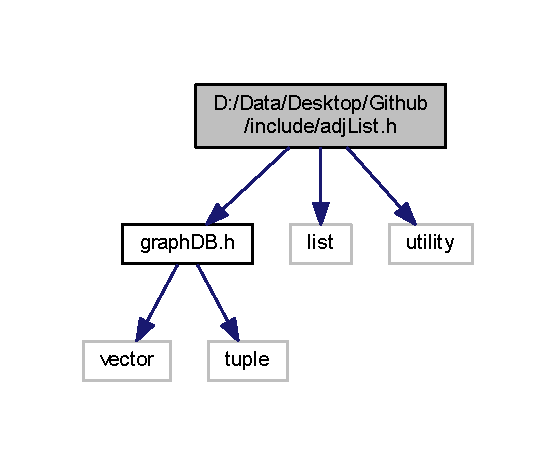
\includegraphics[width=267pt]{adj_list_8h__incl}
\end{center}
\end{figure}
This graph shows which files directly or indirectly include this file\+:\nopagebreak
\begin{figure}[H]
\begin{center}
\leavevmode
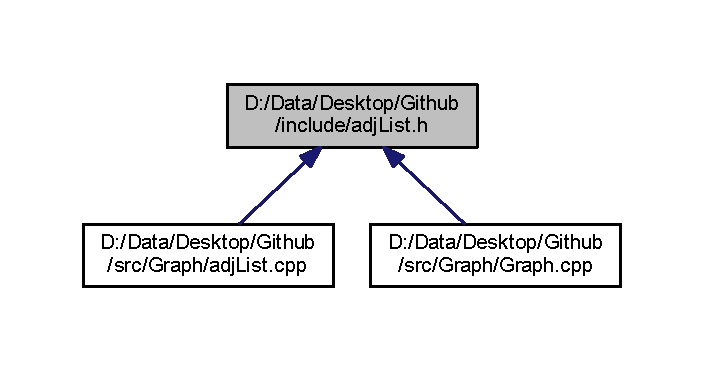
\includegraphics[width=338pt]{adj_list_8h__dep__incl}
\end{center}
\end{figure}
\subsection*{Classes}
\begin{DoxyCompactItemize}
\item 
class \hyperlink{class_alg_lib_1_1adj_list}{Alg\+Lib\+::adj\+List}
\end{DoxyCompactItemize}
\subsection*{Namespaces}
\begin{DoxyCompactItemize}
\item 
 \hyperlink{namespace_alg_lib}{Alg\+Lib}
\end{DoxyCompactItemize}
\subsection*{Macros}
\begin{DoxyCompactItemize}
\item 
\#define \hyperlink{adj_list_8h_a51f31da49b1e5d916bfac8fe47666bc9}{A\+D\+J\+L\+I\+S\+T\+\_\+H}
\end{DoxyCompactItemize}


\subsection{Macro Definition Documentation}
\index{adj\+List.\+h@{adj\+List.\+h}!A\+D\+J\+L\+I\+S\+T\+\_\+H@{A\+D\+J\+L\+I\+S\+T\+\_\+H}}
\index{A\+D\+J\+L\+I\+S\+T\+\_\+H@{A\+D\+J\+L\+I\+S\+T\+\_\+H}!adj\+List.\+h@{adj\+List.\+h}}
\subsubsection[{\texorpdfstring{A\+D\+J\+L\+I\+S\+T\+\_\+H}{ADJLIST_H}}]{\setlength{\rightskip}{0pt plus 5cm}\#define A\+D\+J\+L\+I\+S\+T\+\_\+H}\hypertarget{adj_list_8h_a51f31da49b1e5d916bfac8fe47666bc9}{}\label{adj_list_8h_a51f31da49b1e5d916bfac8fe47666bc9}


Definition at line 3 of file adj\+List.\+h.


\hypertarget{adj_matrix_8h}{}\section{D\+:/\+Data/\+Desktop/\+Github/include/adj\+Matrix.h File Reference}
\label{adj_matrix_8h}\index{D\+:/\+Data/\+Desktop/\+Github/include/adj\+Matrix.\+h@{D\+:/\+Data/\+Desktop/\+Github/include/adj\+Matrix.\+h}}
{\ttfamily \#include \char`\"{}graph\+D\+B.\+h\char`\"{}}\\*
{\ttfamily \#include \char`\"{}Matrix.\+h\char`\"{}}\\*
{\ttfamily \#include $<$vector$>$}\\*
{\ttfamily \#include $<$tuple$>$}\\*
Include dependency graph for adj\+Matrix.\+h\+:\nopagebreak
\begin{figure}[H]
\begin{center}
\leavevmode
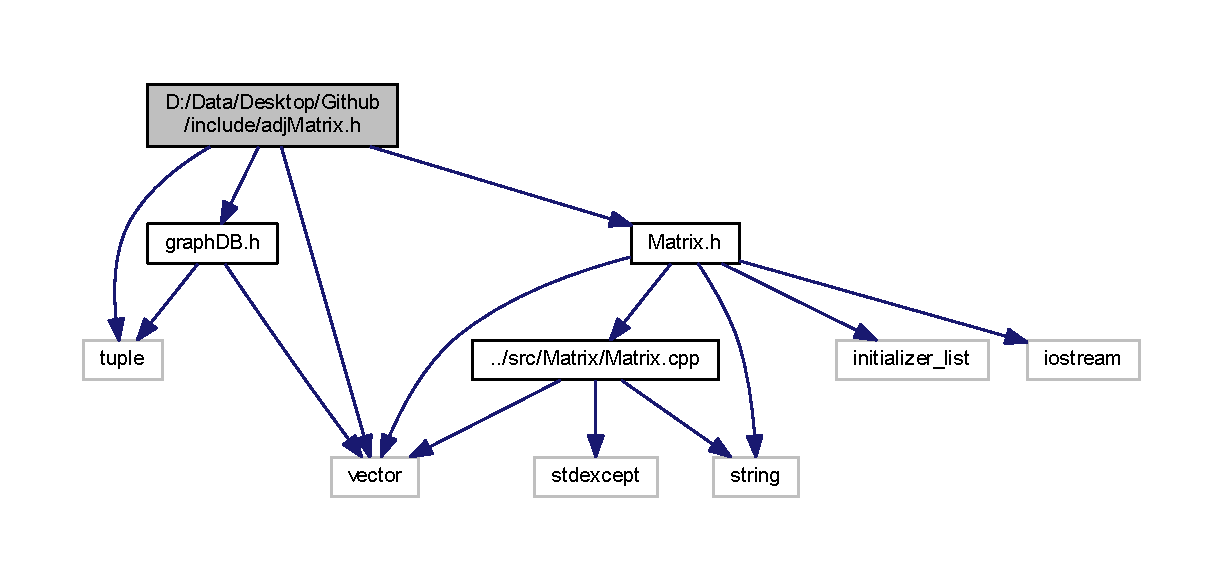
\includegraphics[width=350pt]{adj_matrix_8h__incl}
\end{center}
\end{figure}
This graph shows which files directly or indirectly include this file\+:\nopagebreak
\begin{figure}[H]
\begin{center}
\leavevmode
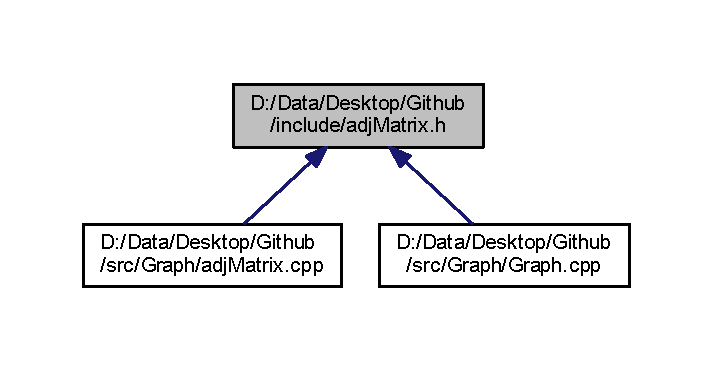
\includegraphics[width=342pt]{adj_matrix_8h__dep__incl}
\end{center}
\end{figure}
\subsection*{Classes}
\begin{DoxyCompactItemize}
\item 
class \hyperlink{class_alg_lib_1_1adj_matrix}{Alg\+Lib\+::adj\+Matrix}
\end{DoxyCompactItemize}
\subsection*{Namespaces}
\begin{DoxyCompactItemize}
\item 
 \hyperlink{namespace_alg_lib}{Alg\+Lib}
\end{DoxyCompactItemize}

\hypertarget{_fraction_8h}{}\section{D\+:/\+Data/\+Desktop/\+Github/include/\+Fraction.h File Reference}
\label{_fraction_8h}\index{D\+:/\+Data/\+Desktop/\+Github/include/\+Fraction.\+h@{D\+:/\+Data/\+Desktop/\+Github/include/\+Fraction.\+h}}
{\ttfamily \#include $<$string$>$}\\*
Include dependency graph for Fraction.\+h\+:\nopagebreak
\begin{figure}[H]
\begin{center}
\leavevmode
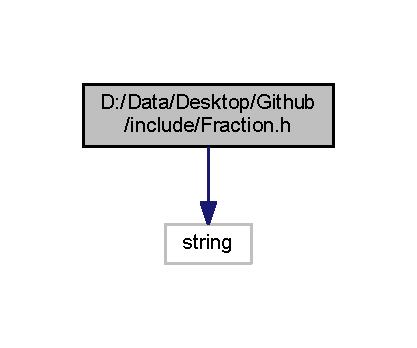
\includegraphics[width=200pt]{_fraction_8h__incl}
\end{center}
\end{figure}
This graph shows which files directly or indirectly include this file\+:\nopagebreak
\begin{figure}[H]
\begin{center}
\leavevmode
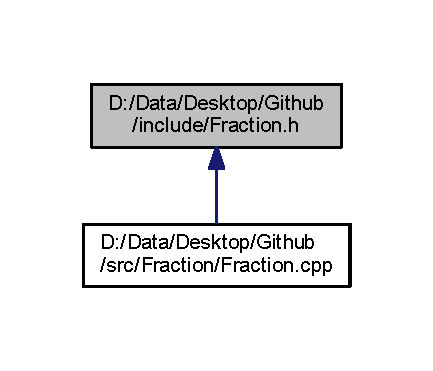
\includegraphics[width=208pt]{_fraction_8h__dep__incl}
\end{center}
\end{figure}
\subsection*{Classes}
\begin{DoxyCompactItemize}
\item 
class \hyperlink{class_alg_lib_1_1_fraction}{Alg\+Lib\+::\+Fraction}
\end{DoxyCompactItemize}
\subsection*{Namespaces}
\begin{DoxyCompactItemize}
\item 
 \hyperlink{namespace_alg_lib}{Alg\+Lib}
\end{DoxyCompactItemize}

\hypertarget{_graph_8h}{}\section{D\+:/\+Data/\+Desktop/\+Github/include/\+Graph.h File Reference}
\label{_graph_8h}\index{D\+:/\+Data/\+Desktop/\+Github/include/\+Graph.\+h@{D\+:/\+Data/\+Desktop/\+Github/include/\+Graph.\+h}}
{\ttfamily \#include \char`\"{}graph\+D\+B.\+h\char`\"{}}\\*
{\ttfamily \#include \char`\"{}Matrix.\+h\char`\"{}}\\*
{\ttfamily \#include $<$vector$>$}\\*
{\ttfamily \#include $<$tuple$>$}\\*
{\ttfamily \#include $<$initializer\+\_\+list$>$}\\*
Include dependency graph for Graph.\+h\+:\nopagebreak
\begin{figure}[H]
\begin{center}
\leavevmode
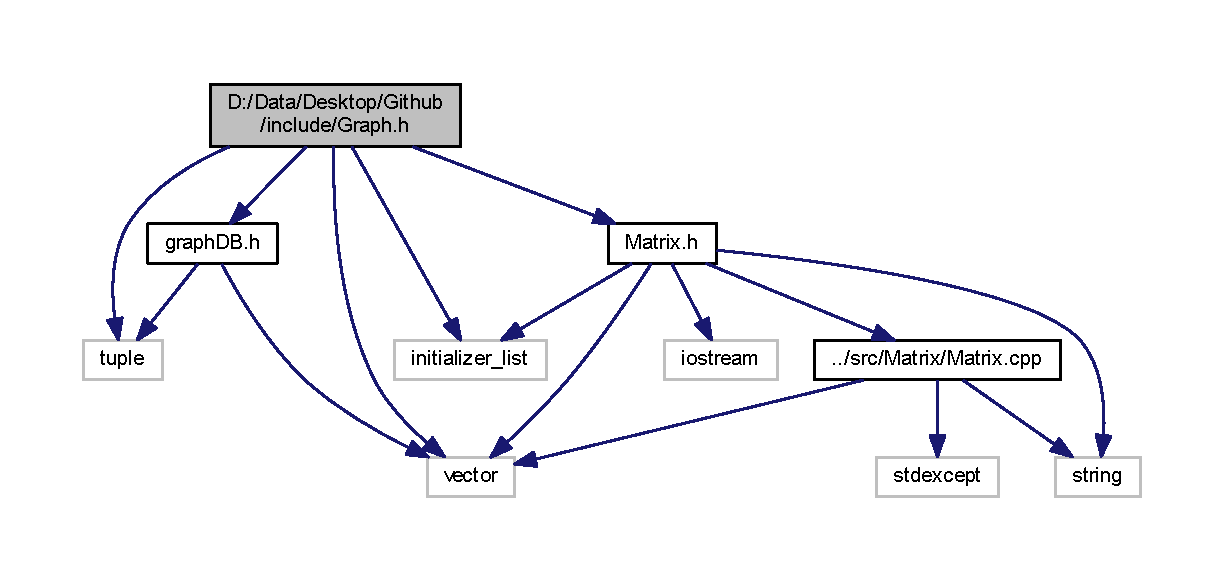
\includegraphics[width=350pt]{_graph_8h__incl}
\end{center}
\end{figure}
This graph shows which files directly or indirectly include this file\+:\nopagebreak
\begin{figure}[H]
\begin{center}
\leavevmode
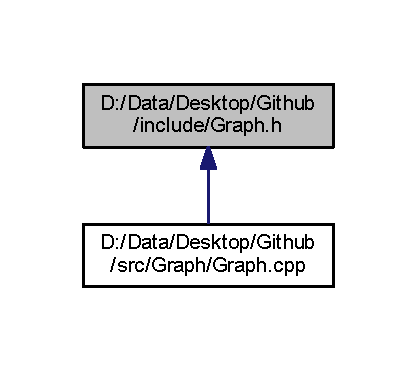
\includegraphics[width=200pt]{_graph_8h__dep__incl}
\end{center}
\end{figure}
\subsection*{Classes}
\begin{DoxyCompactItemize}
\item 
class \hyperlink{class_alg_lib_1_1_graph}{Alg\+Lib\+::\+Graph}
\end{DoxyCompactItemize}
\subsection*{Namespaces}
\begin{DoxyCompactItemize}
\item 
 \hyperlink{namespace_alg_lib}{Alg\+Lib}
\end{DoxyCompactItemize}
\subsection*{Enumerations}
\begin{DoxyCompactItemize}
\item 
enum \hyperlink{namespace_alg_lib_a11966d2ea6c430adfb83a6ebaa05e337}{Alg\+Lib\+::db\+Type} \{ \hyperlink{namespace_alg_lib_a11966d2ea6c430adfb83a6ebaa05e337a9d8e68c3898f769422174fed0be93fd2}{Alg\+Lib\+::db\+Type\+::\+A\+D\+J\+A\+C\+E\+N\+C\+Y\+\_\+\+M\+A\+T\+R\+IX}, 
\hyperlink{namespace_alg_lib_a11966d2ea6c430adfb83a6ebaa05e337a6d02e698876f8aa2b2e975e8c0010c10}{Alg\+Lib\+::db\+Type\+::\+A\+D\+J\+A\+C\+E\+N\+C\+Y\+\_\+\+L\+I\+ST}
 \}
\end{DoxyCompactItemize}

\hypertarget{graph_d_b_8h}{}\section{D\+:/\+Data/\+Desktop/\+Github/include/graph\+DB.h File Reference}
\label{graph_d_b_8h}\index{D\+:/\+Data/\+Desktop/\+Github/include/graph\+D\+B.\+h@{D\+:/\+Data/\+Desktop/\+Github/include/graph\+D\+B.\+h}}
{\ttfamily \#include $<$vector$>$}\\*
{\ttfamily \#include $<$tuple$>$}\\*
Include dependency graph for graph\+D\+B.\+h\+:\nopagebreak
\begin{figure}[H]
\begin{center}
\leavevmode
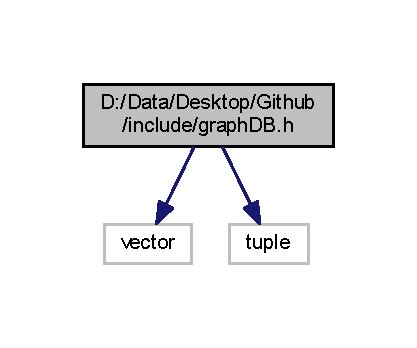
\includegraphics[width=200pt]{graph_d_b_8h__incl}
\end{center}
\end{figure}
This graph shows which files directly or indirectly include this file\+:\nopagebreak
\begin{figure}[H]
\begin{center}
\leavevmode
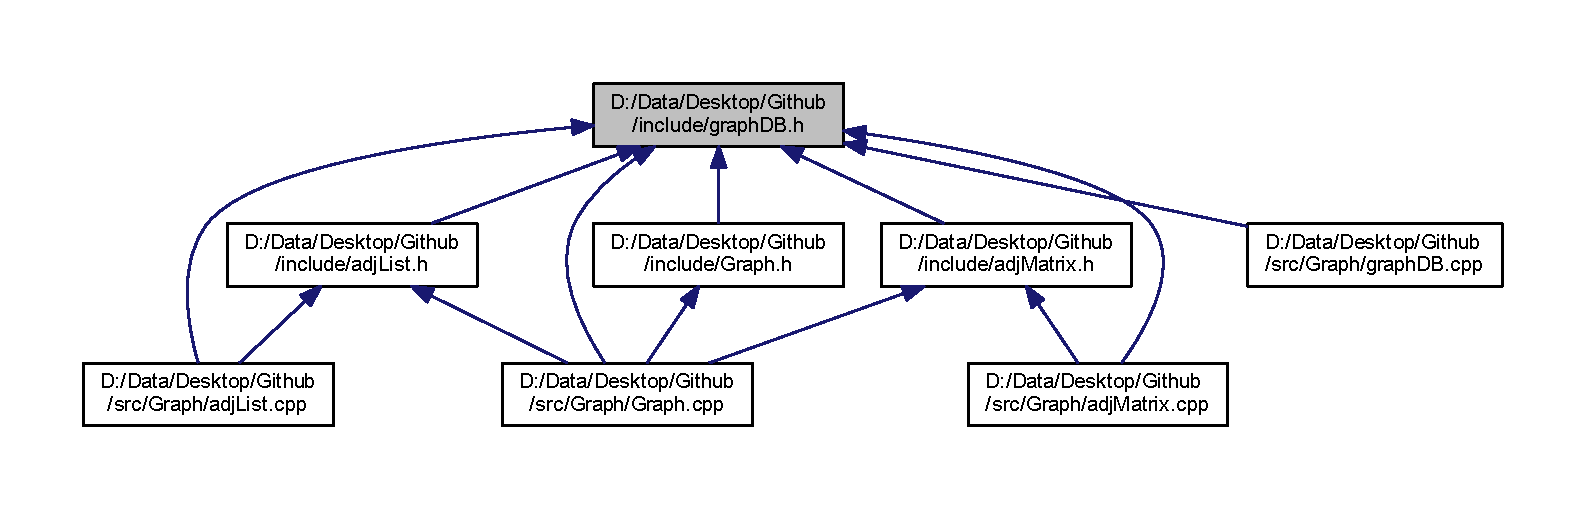
\includegraphics[width=350pt]{graph_d_b_8h__dep__incl}
\end{center}
\end{figure}
\subsection*{Classes}
\begin{DoxyCompactItemize}
\item 
class \hyperlink{class_alg_lib_1_1graph_d_b}{Alg\+Lib\+::graph\+DB}
\end{DoxyCompactItemize}
\subsection*{Namespaces}
\begin{DoxyCompactItemize}
\item 
 \hyperlink{namespace_alg_lib}{Alg\+Lib}
\end{DoxyCompactItemize}

\hypertarget{_heap_8h}{}\section{D\+:/\+Data/\+Desktop/\+Github/include/\+Heap.h File Reference}
\label{_heap_8h}\index{D\+:/\+Data/\+Desktop/\+Github/include/\+Heap.\+h@{D\+:/\+Data/\+Desktop/\+Github/include/\+Heap.\+h}}
{\ttfamily \#include $<$vector$>$}\\*
{\ttfamily \#include $<$initializer\+\_\+list$>$}\\*
{\ttfamily \#include $<$functional$>$}\\*
{\ttfamily \#include \char`\"{}../src/\+Heap/\+Heap.\+cpp\char`\"{}}\\*
Include dependency graph for Heap.\+h\+:\nopagebreak
\begin{figure}[H]
\begin{center}
\leavevmode
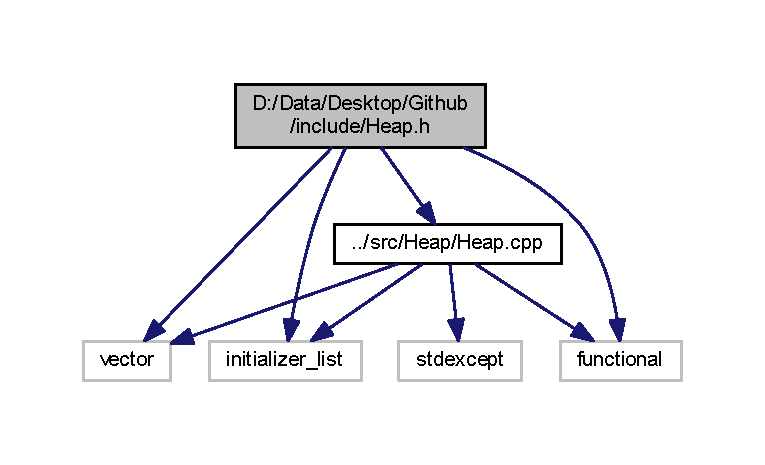
\includegraphics[width=350pt]{_heap_8h__incl}
\end{center}
\end{figure}
This graph shows which files directly or indirectly include this file\+:\nopagebreak
\begin{figure}[H]
\begin{center}
\leavevmode
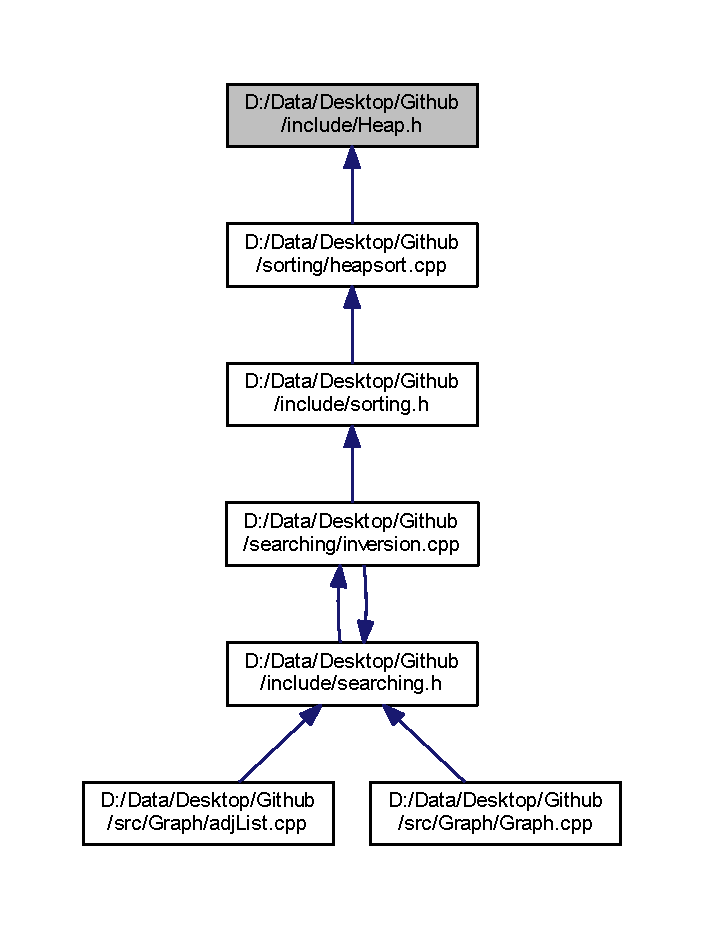
\includegraphics[width=338pt]{_heap_8h__dep__incl}
\end{center}
\end{figure}
\subsection*{Classes}
\begin{DoxyCompactItemize}
\item 
class \hyperlink{class_alg_lib_1_1_heap}{Alg\+Lib\+::\+Heap$<$ T $>$}
\end{DoxyCompactItemize}
\subsection*{Namespaces}
\begin{DoxyCompactItemize}
\item 
 \hyperlink{namespace_alg_lib}{Alg\+Lib}
\end{DoxyCompactItemize}

\hypertarget{_matrix_8h}{}\section{D\+:/\+Data/\+Desktop/\+Github/include/\+Matrix.h File Reference}
\label{_matrix_8h}\index{D\+:/\+Data/\+Desktop/\+Github/include/\+Matrix.\+h@{D\+:/\+Data/\+Desktop/\+Github/include/\+Matrix.\+h}}
{\ttfamily \#include $<$initializer\+\_\+list$>$}\\*
{\ttfamily \#include $<$vector$>$}\\*
{\ttfamily \#include $<$iostream$>$}\\*
{\ttfamily \#include $<$string$>$}\\*
{\ttfamily \#include \char`\"{}../src/\+Matrix/\+Matrix.\+cpp\char`\"{}}\\*
Include dependency graph for Matrix.\+h\+:\nopagebreak
\begin{figure}[H]
\begin{center}
\leavevmode
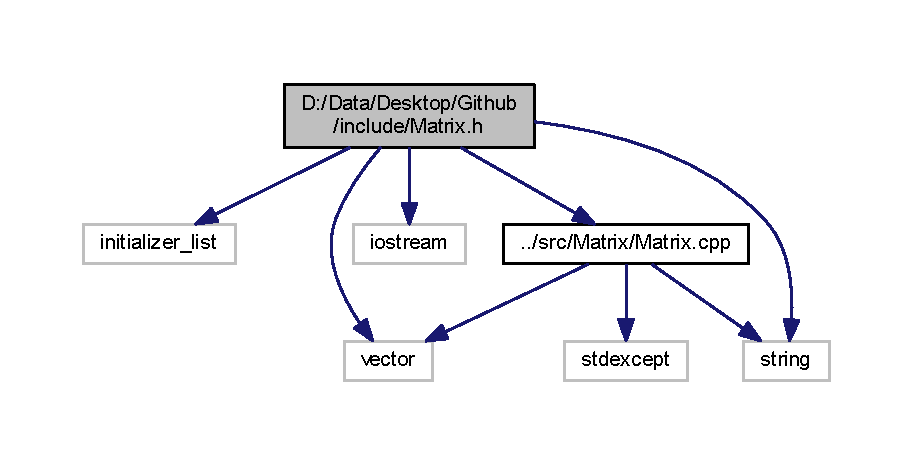
\includegraphics[width=350pt]{_matrix_8h__incl}
\end{center}
\end{figure}
This graph shows which files directly or indirectly include this file\+:\nopagebreak
\begin{figure}[H]
\begin{center}
\leavevmode
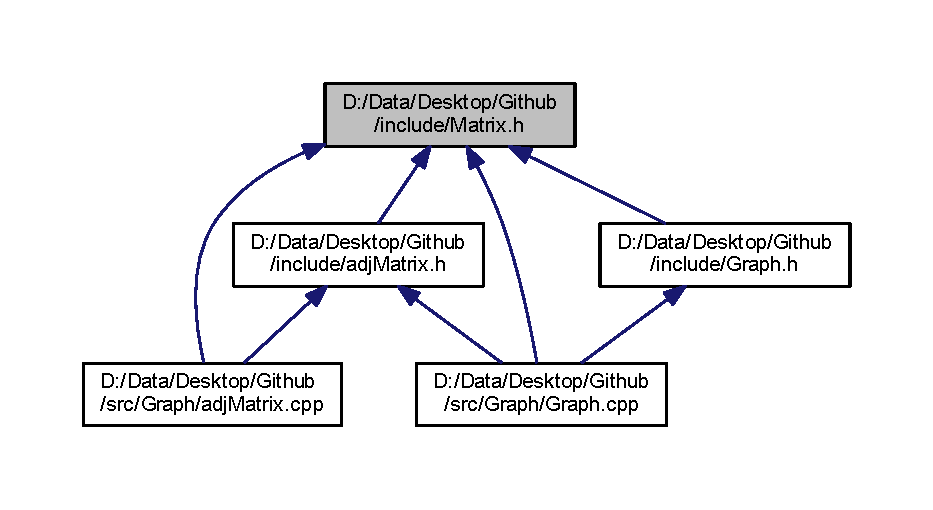
\includegraphics[width=350pt]{_matrix_8h__dep__incl}
\end{center}
\end{figure}
\subsection*{Classes}
\begin{DoxyCompactItemize}
\item 
class \hyperlink{class_alg_lib_1_1_matrix}{Alg\+Lib\+::\+Matrix$<$ T $>$}
\end{DoxyCompactItemize}
\subsection*{Namespaces}
\begin{DoxyCompactItemize}
\item 
 \hyperlink{namespace_alg_lib}{Alg\+Lib}
\end{DoxyCompactItemize}

\hypertarget{_permutation_8h}{}\section{D\+:/\+Data/\+Desktop/\+Github/include/\+Permutation.h File Reference}
\label{_permutation_8h}\index{D\+:/\+Data/\+Desktop/\+Github/include/\+Permutation.\+h@{D\+:/\+Data/\+Desktop/\+Github/include/\+Permutation.\+h}}
{\ttfamily \#include $<$initializer\+\_\+list$>$}\\*
{\ttfamily \#include $<$vector$>$}\\*
{\ttfamily \#include $<$utility$>$}\\*
{\ttfamily \#include \char`\"{}../src/\+Permutation/\+Permutation.\+cpp\char`\"{}}\\*
Include dependency graph for Permutation.\+h\+:\nopagebreak
\begin{figure}[H]
\begin{center}
\leavevmode
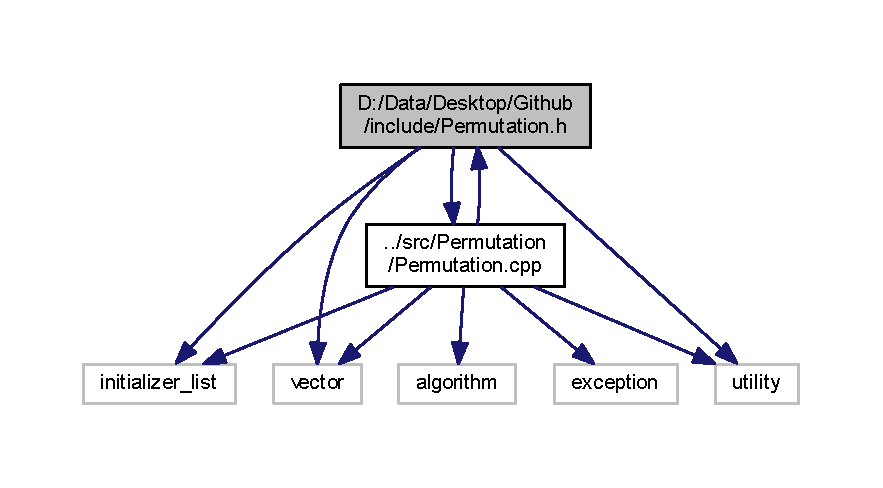
\includegraphics[width=350pt]{_permutation_8h__incl}
\end{center}
\end{figure}
This graph shows which files directly or indirectly include this file\+:\nopagebreak
\begin{figure}[H]
\begin{center}
\leavevmode
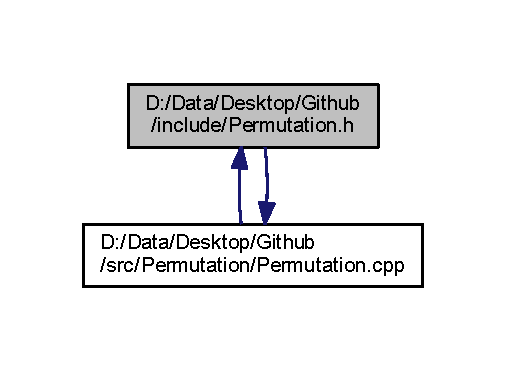
\includegraphics[width=243pt]{_permutation_8h__dep__incl}
\end{center}
\end{figure}
\subsection*{Classes}
\begin{DoxyCompactItemize}
\item 
class \hyperlink{class_alg_lib_1_1_permutation}{Alg\+Lib\+::\+Permutation$<$ T $>$}
\end{DoxyCompactItemize}
\subsection*{Namespaces}
\begin{DoxyCompactItemize}
\item 
 \hyperlink{namespace_alg_lib}{Alg\+Lib}
\end{DoxyCompactItemize}

\hypertarget{_polynomial_8h}{}\section{D\+:/\+Data/\+Desktop/\+Github/include/\+Polynomial.h File Reference}
\label{_polynomial_8h}\index{D\+:/\+Data/\+Desktop/\+Github/include/\+Polynomial.\+h@{D\+:/\+Data/\+Desktop/\+Github/include/\+Polynomial.\+h}}
{\ttfamily \#include $<$vector$>$}\\*
{\ttfamily \#include $<$initializer\+\_\+list$>$}\\*
{\ttfamily \#include \char`\"{}../src/\+Polynomial/\+Polynomial.\+cpp\char`\"{}}\\*
Include dependency graph for Polynomial.\+h\+:\nopagebreak
\begin{figure}[H]
\begin{center}
\leavevmode
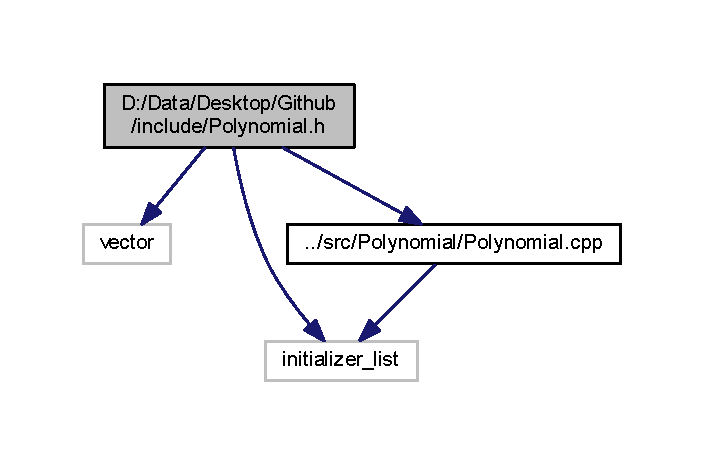
\includegraphics[width=338pt]{_polynomial_8h__incl}
\end{center}
\end{figure}
This graph shows which files directly or indirectly include this file\+:\nopagebreak
\begin{figure}[H]
\begin{center}
\leavevmode
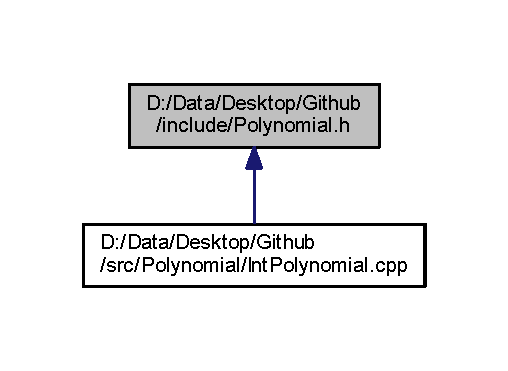
\includegraphics[width=244pt]{_polynomial_8h__dep__incl}
\end{center}
\end{figure}
\subsection*{Classes}
\begin{DoxyCompactItemize}
\item 
class \hyperlink{class_alg_lib_1_1_polynomial}{Alg\+Lib\+::\+Polynomial$<$ coeff $>$}
\item 
class \hyperlink{class_alg_lib_1_1_integer_polynomial}{Alg\+Lib\+::\+Integer\+Polynomial}
\end{DoxyCompactItemize}
\subsection*{Namespaces}
\begin{DoxyCompactItemize}
\item 
 \hyperlink{namespace_alg_lib}{Alg\+Lib}
\end{DoxyCompactItemize}

\hypertarget{searching_8h}{}\section{D\+:/\+Data/\+Desktop/\+Github/include/searching.h File Reference}
\label{searching_8h}\index{D\+:/\+Data/\+Desktop/\+Github/include/searching.\+h@{D\+:/\+Data/\+Desktop/\+Github/include/searching.\+h}}
{\ttfamily \#include \char`\"{}../searching/binarysearch.\+cpp\char`\"{}}\\*
{\ttfamily \#include \char`\"{}../searching/inversion.\+cpp\char`\"{}}\\*
Include dependency graph for searching.\+h\+:\nopagebreak
\begin{figure}[H]
\begin{center}
\leavevmode
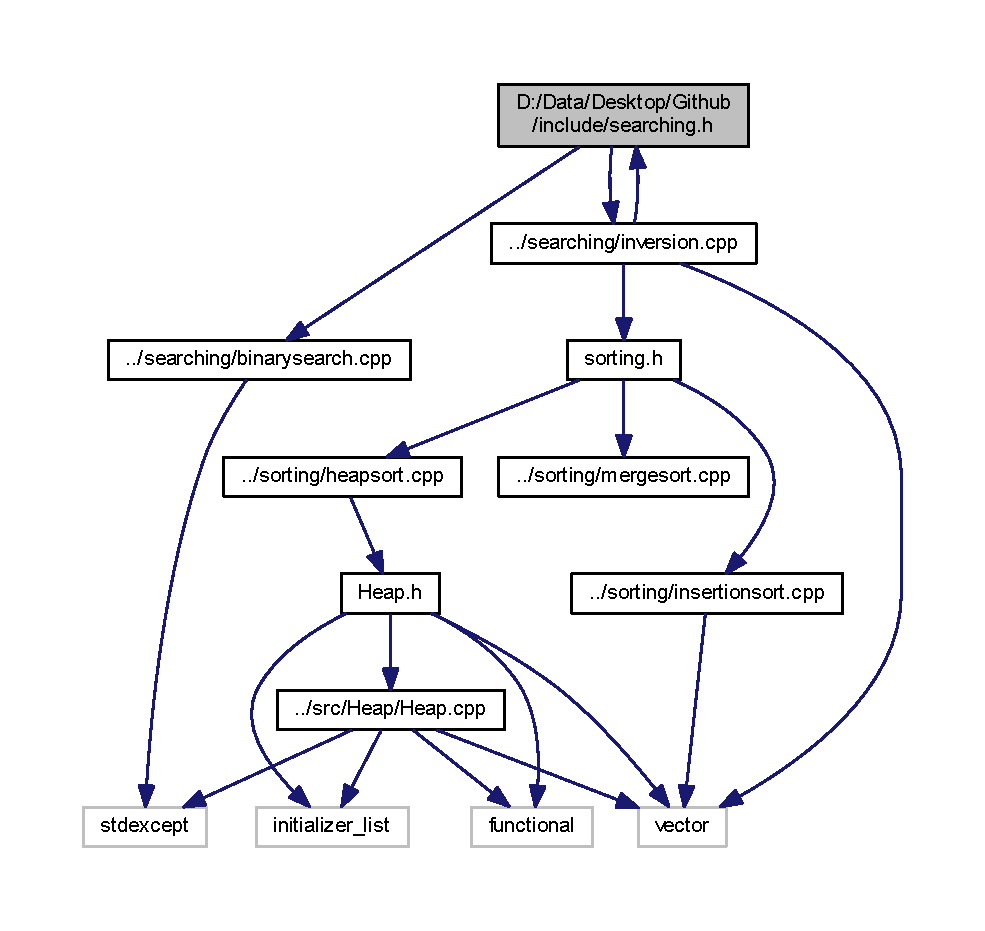
\includegraphics[width=350pt]{searching_8h__incl}
\end{center}
\end{figure}
This graph shows which files directly or indirectly include this file\+:\nopagebreak
\begin{figure}[H]
\begin{center}
\leavevmode
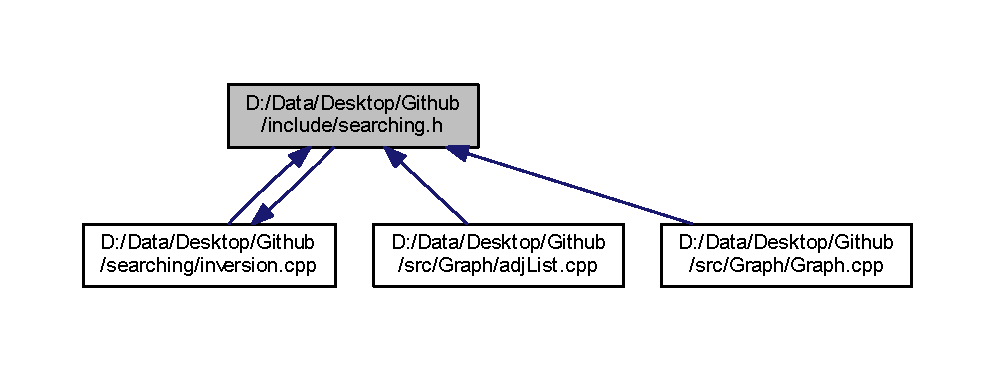
\includegraphics[width=350pt]{searching_8h__dep__incl}
\end{center}
\end{figure}
\subsection*{Namespaces}
\begin{DoxyCompactItemize}
\item 
 \hyperlink{namespace_alg_lib}{Alg\+Lib}
\end{DoxyCompactItemize}
\subsection*{Functions}
\begin{DoxyCompactItemize}
\item 
{\footnotesize template$<$typename cont , typename T $>$ }\\int \hyperlink{namespace_alg_lib_a42bfc6dd0232e3e7d0a460a5bb74059a}{Alg\+Lib\+::binarysearch} (cont A, T key)
\begin{DoxyCompactList}\small\item\em Searches a sorted container A for an element key. \end{DoxyCompactList}\item 
{\footnotesize template$<$typename cont $>$ }\\int \hyperlink{namespace_alg_lib_a97a13becf845332c126803e014b03286}{Alg\+Lib\+::inversions} (const cont \&A)
\begin{DoxyCompactList}\small\item\em Counts the number of inversions in a container A. An inversion is a pair of elements A\mbox{[}i\mbox{]} and A\mbox{[}j\mbox{]} such that i $<$ j and A\mbox{[}i\mbox{]} $>$ A\mbox{[}j\mbox{]}. Finds in O(n log n) time. \end{DoxyCompactList}\end{DoxyCompactItemize}

\hypertarget{sorting_8h}{}\section{D\+:/\+Data/\+Desktop/\+Github/include/sorting.h File Reference}
\label{sorting_8h}\index{D\+:/\+Data/\+Desktop/\+Github/include/sorting.\+h@{D\+:/\+Data/\+Desktop/\+Github/include/sorting.\+h}}
{\ttfamily \#include \char`\"{}../sorting/insertionsort.\+cpp\char`\"{}}\\*
{\ttfamily \#include \char`\"{}../sorting/mergesort.\+cpp\char`\"{}}\\*
{\ttfamily \#include \char`\"{}../sorting/heapsort.\+cpp\char`\"{}}\\*
Include dependency graph for sorting.\+h\+:\nopagebreak
\begin{figure}[H]
\begin{center}
\leavevmode
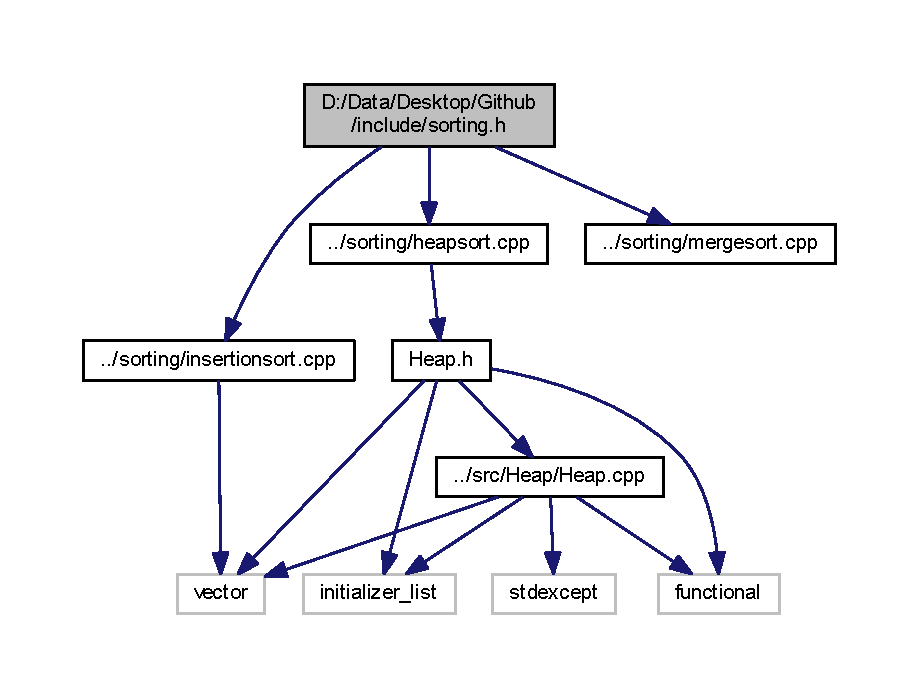
\includegraphics[width=350pt]{sorting_8h__incl}
\end{center}
\end{figure}
This graph shows which files directly or indirectly include this file\+:\nopagebreak
\begin{figure}[H]
\begin{center}
\leavevmode
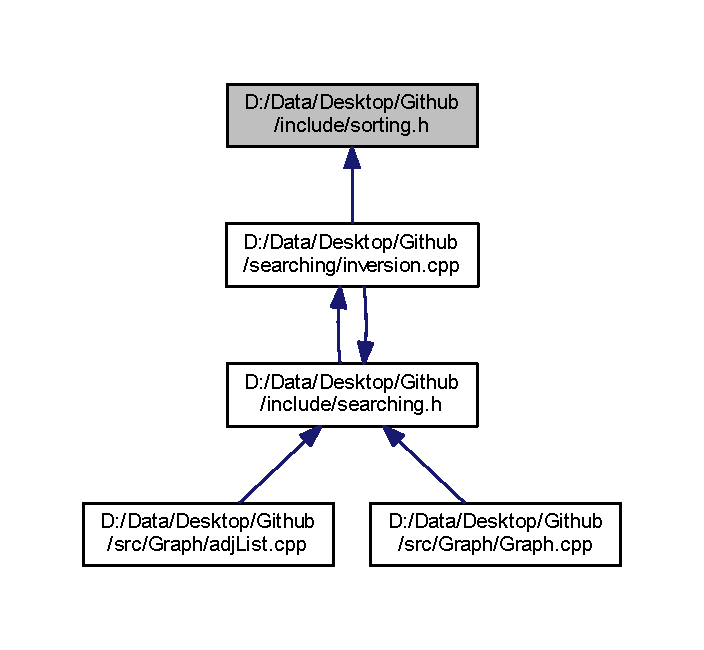
\includegraphics[width=338pt]{sorting_8h__dep__incl}
\end{center}
\end{figure}
\subsection*{Namespaces}
\begin{DoxyCompactItemize}
\item 
 \hyperlink{namespace_alg_lib}{Alg\+Lib}
\end{DoxyCompactItemize}
\subsection*{Functions}
\begin{DoxyCompactItemize}
\item 
{\footnotesize template$<$typename T $>$ }\\void \hyperlink{namespace_alg_lib_a285a3cda7220504508dbb7d0df3dba21}{Alg\+Lib\+::insertion\+Sort} (T \&arr)
\item 
{\footnotesize template$<$typename T $>$ }\\void \hyperlink{namespace_alg_lib_a50103bb855668c829f3d0def288521a8}{Alg\+Lib\+::merge\+Sort} (T \&arr)
\begin{DoxyCompactList}\small\item\em Sort the elements in container arr with merge sort algorithm. \end{DoxyCompactList}\item 
{\footnotesize template$<$typename T $>$ }\\T \hyperlink{namespace_alg_lib_a964728cae397746308b2d688e6f85d01}{Alg\+Lib\+::\+M\+E\+R\+GE} (T \&left, T \&right)
\item 
{\footnotesize template$<$typename T , typename S $>$ }\\void \hyperlink{namespace_alg_lib_a09ea4c537af6d2dcc36a9753b7af7c05}{Alg\+Lib\+::heap\+Sort} (T \&arr)
\end{DoxyCompactItemize}

\hypertarget{_r_e_a_d_m_e_8md}{}\section{D\+:/\+Data/\+Desktop/\+Github/\+R\+E\+A\+D\+ME.md File Reference}
\label{_r_e_a_d_m_e_8md}\index{D\+:/\+Data/\+Desktop/\+Github/\+R\+E\+A\+D\+M\+E.\+md@{D\+:/\+Data/\+Desktop/\+Github/\+R\+E\+A\+D\+M\+E.\+md}}

\hypertarget{binarysearch_8cpp}{}\section{D\+:/\+Data/\+Desktop/\+Github/searching/binarysearch.cpp File Reference}
\label{binarysearch_8cpp}\index{D\+:/\+Data/\+Desktop/\+Github/searching/binarysearch.\+cpp@{D\+:/\+Data/\+Desktop/\+Github/searching/binarysearch.\+cpp}}
{\ttfamily \#include $<$stdexcept$>$}\\*
Include dependency graph for binarysearch.\+cpp\+:\nopagebreak
\begin{figure}[H]
\begin{center}
\leavevmode
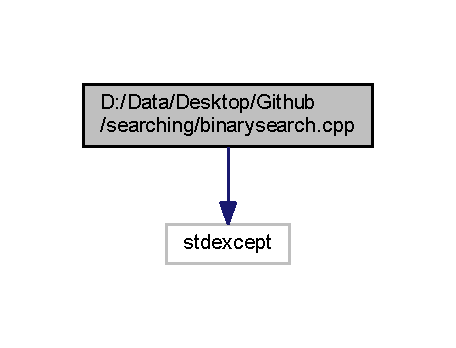
\includegraphics[width=219pt]{binarysearch_8cpp__incl}
\end{center}
\end{figure}
This graph shows which files directly or indirectly include this file\+:\nopagebreak
\begin{figure}[H]
\begin{center}
\leavevmode
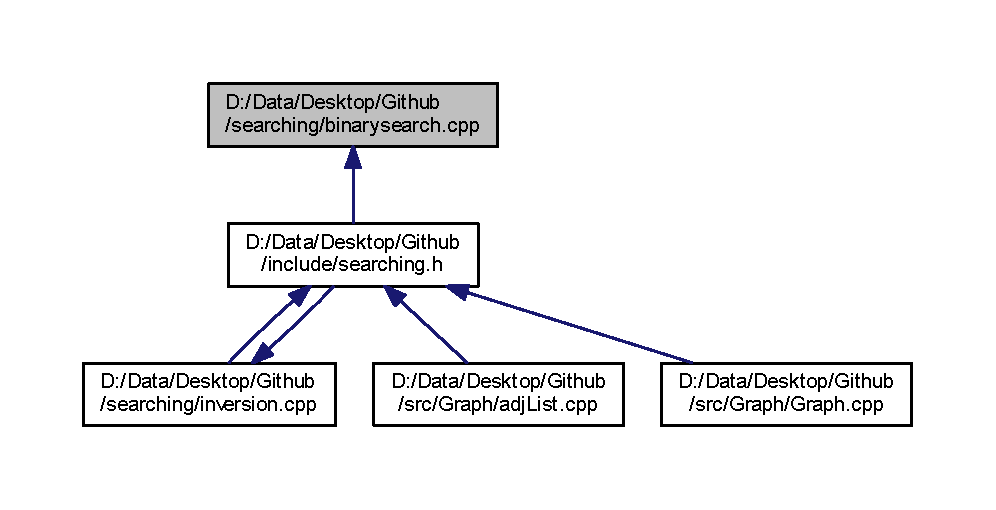
\includegraphics[width=350pt]{binarysearch_8cpp__dep__incl}
\end{center}
\end{figure}
\subsection*{Namespaces}
\begin{DoxyCompactItemize}
\item 
 \hyperlink{namespace_alg_lib}{Alg\+Lib}
\end{DoxyCompactItemize}
\subsection*{Functions}
\begin{DoxyCompactItemize}
\item 
{\footnotesize template$<$typename cont , typename T $>$ }\\int \hyperlink{namespace_alg_lib_a42bfc6dd0232e3e7d0a460a5bb74059a}{Alg\+Lib\+::binarysearch} (cont A, T key)
\begin{DoxyCompactList}\small\item\em Searches a sorted container A for an element key. \end{DoxyCompactList}\end{DoxyCompactItemize}

\hypertarget{inversion_8cpp}{}\section{D\+:/\+Data/\+Desktop/\+Github/searching/inversion.cpp File Reference}
\label{inversion_8cpp}\index{D\+:/\+Data/\+Desktop/\+Github/searching/inversion.\+cpp@{D\+:/\+Data/\+Desktop/\+Github/searching/inversion.\+cpp}}
{\ttfamily \#include \char`\"{}sorting.\+h\char`\"{}}\\*
{\ttfamily \#include \char`\"{}searching.\+h\char`\"{}}\\*
{\ttfamily \#include $<$vector$>$}\\*
Include dependency graph for inversion.\+cpp\+:\nopagebreak
\begin{figure}[H]
\begin{center}
\leavevmode
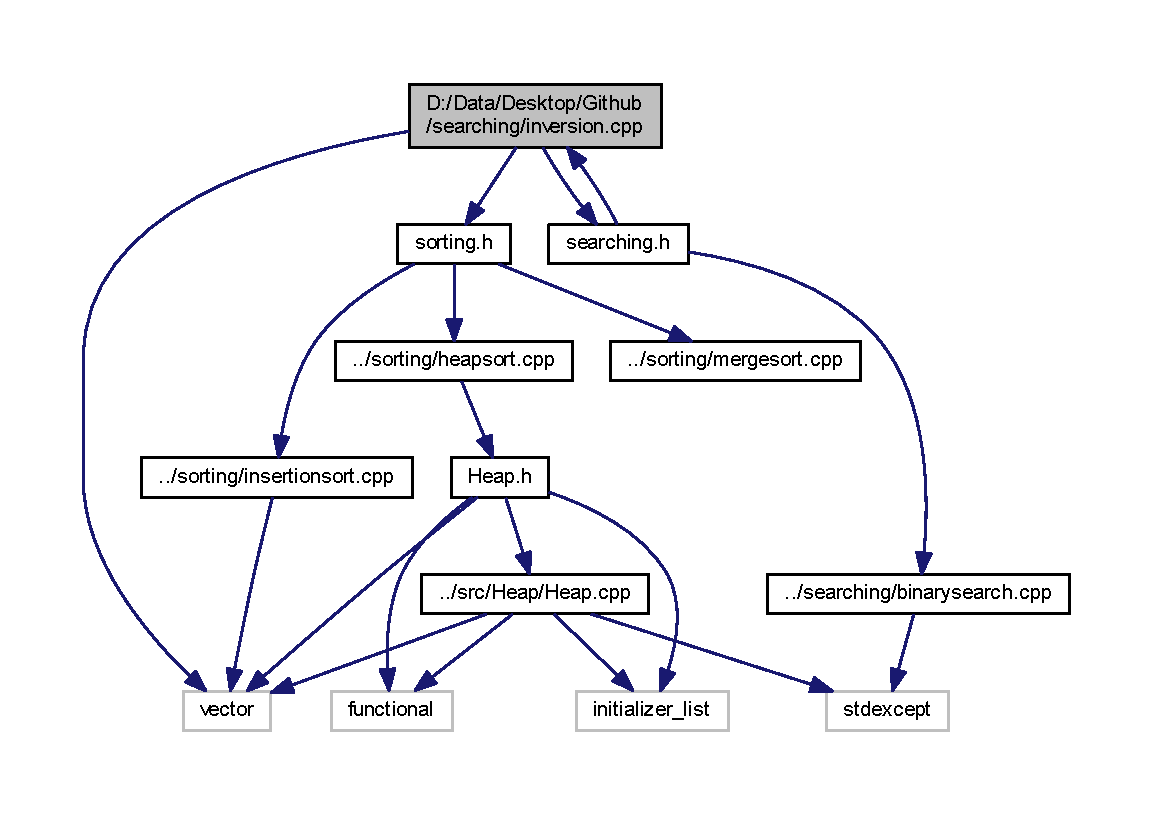
\includegraphics[width=350pt]{inversion_8cpp__incl}
\end{center}
\end{figure}
This graph shows which files directly or indirectly include this file\+:\nopagebreak
\begin{figure}[H]
\begin{center}
\leavevmode
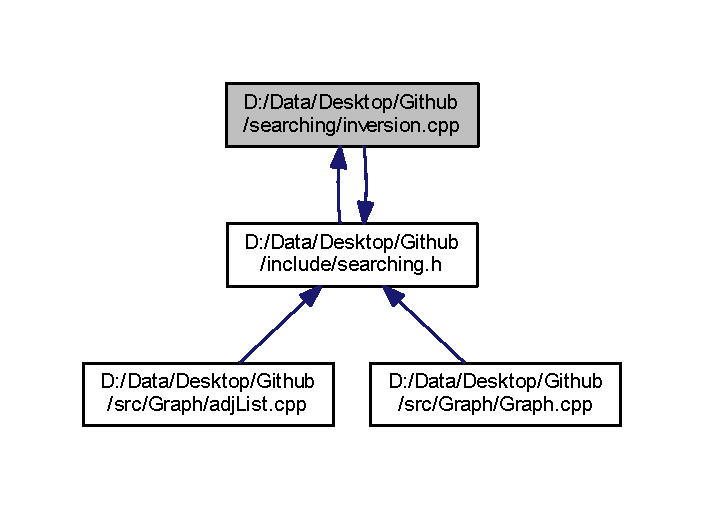
\includegraphics[width=338pt]{inversion_8cpp__dep__incl}
\end{center}
\end{figure}
\subsection*{Namespaces}
\begin{DoxyCompactItemize}
\item 
 \hyperlink{namespace_alg_lib}{Alg\+Lib}
\end{DoxyCompactItemize}
\subsection*{Functions}
\begin{DoxyCompactItemize}
\item 
{\footnotesize template$<$typename cont $>$ }\\int \hyperlink{namespace_alg_lib_ab90b28703ab96313011a0fc73af136e0}{Alg\+Lib\+::inversion\+Ref} (cont \&A)
\item 
{\footnotesize template$<$typename cont $>$ }\\int \hyperlink{namespace_alg_lib_a97a13becf845332c126803e014b03286}{Alg\+Lib\+::inversions} (const cont \&A)
\begin{DoxyCompactList}\small\item\em Counts the number of inversions in a container A. An inversion is a pair of elements A\mbox{[}i\mbox{]} and A\mbox{[}j\mbox{]} such that i $<$ j and A\mbox{[}i\mbox{]} $>$ A\mbox{[}j\mbox{]}. Finds in O(n log n) time. \end{DoxyCompactList}\end{DoxyCompactItemize}

\hypertarget{heapsort_8cpp}{}\section{D\+:/\+Data/\+Desktop/\+Github/sorting/heapsort.cpp File Reference}
\label{heapsort_8cpp}\index{D\+:/\+Data/\+Desktop/\+Github/sorting/heapsort.\+cpp@{D\+:/\+Data/\+Desktop/\+Github/sorting/heapsort.\+cpp}}
{\ttfamily \#include \char`\"{}Heap.\+h\char`\"{}}\\*
Include dependency graph for heapsort.\+cpp\+:\nopagebreak
\begin{figure}[H]
\begin{center}
\leavevmode
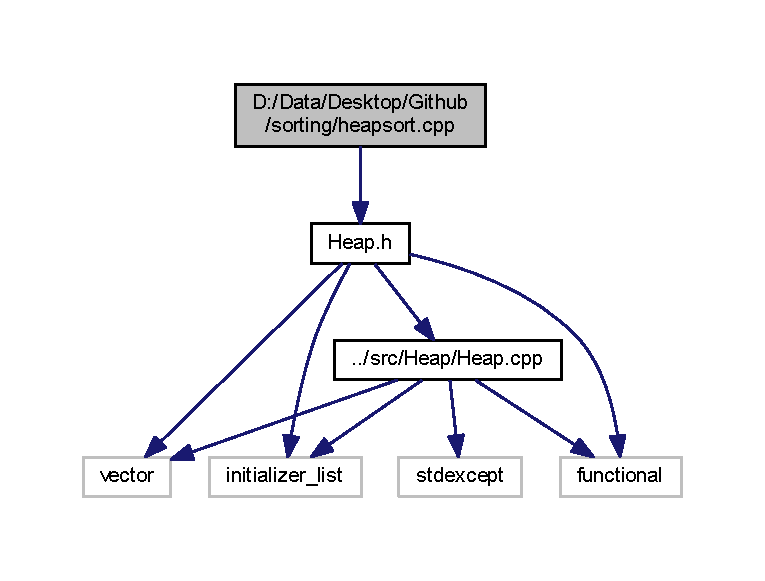
\includegraphics[width=350pt]{heapsort_8cpp__incl}
\end{center}
\end{figure}
This graph shows which files directly or indirectly include this file\+:\nopagebreak
\begin{figure}[H]
\begin{center}
\leavevmode
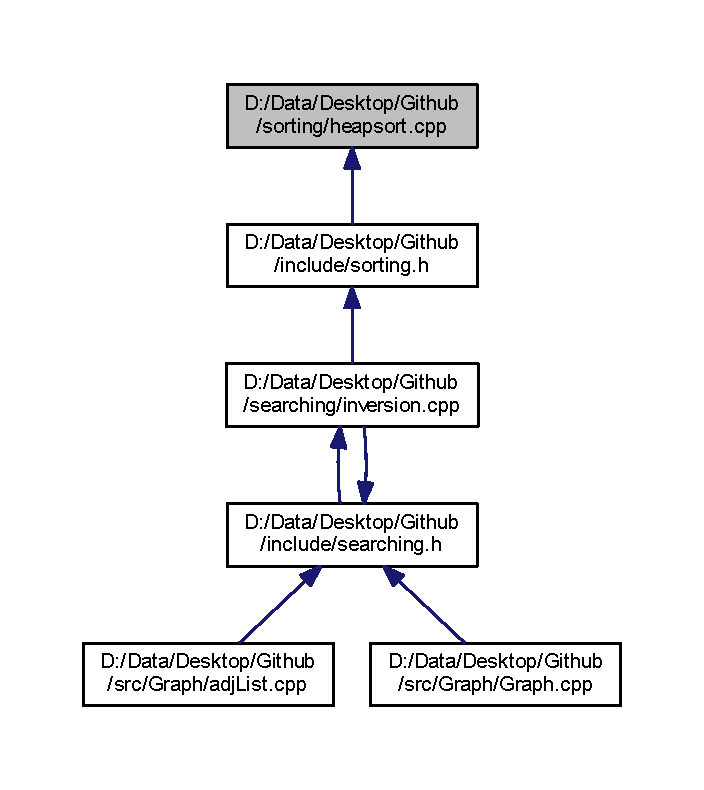
\includegraphics[width=338pt]{heapsort_8cpp__dep__incl}
\end{center}
\end{figure}
\subsection*{Namespaces}
\begin{DoxyCompactItemize}
\item 
 \hyperlink{namespace_alg_lib}{Alg\+Lib}
\end{DoxyCompactItemize}
\subsection*{Functions}
\begin{DoxyCompactItemize}
\item 
{\footnotesize template$<$typename T , typename S $>$ }\\void \hyperlink{namespace_alg_lib_a09ea4c537af6d2dcc36a9753b7af7c05}{Alg\+Lib\+::heap\+Sort} (T \&arr)
\end{DoxyCompactItemize}

\hypertarget{insertionsort_8cpp}{}\section{D\+:/\+Data/\+Desktop/\+Github/sorting/insertionsort.cpp File Reference}
\label{insertionsort_8cpp}\index{D\+:/\+Data/\+Desktop/\+Github/sorting/insertionsort.\+cpp@{D\+:/\+Data/\+Desktop/\+Github/sorting/insertionsort.\+cpp}}
{\ttfamily \#include $<$vector$>$}\\*
Include dependency graph for insertionsort.\+cpp\+:\nopagebreak
\begin{figure}[H]
\begin{center}
\leavevmode
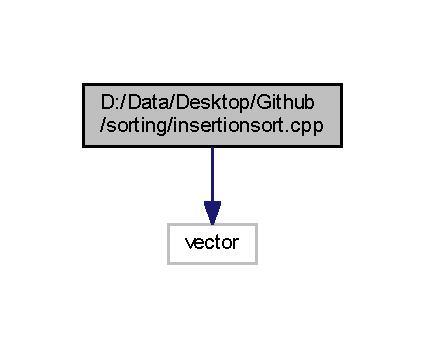
\includegraphics[width=204pt]{insertionsort_8cpp__incl}
\end{center}
\end{figure}
This graph shows which files directly or indirectly include this file\+:\nopagebreak
\begin{figure}[H]
\begin{center}
\leavevmode
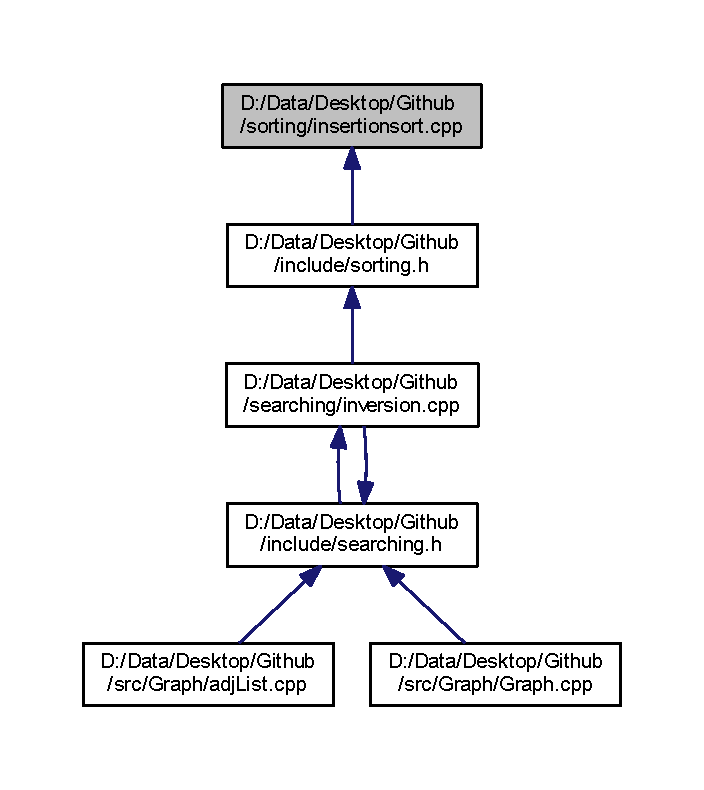
\includegraphics[width=338pt]{insertionsort_8cpp__dep__incl}
\end{center}
\end{figure}
\subsection*{Namespaces}
\begin{DoxyCompactItemize}
\item 
 \hyperlink{namespace_alg_lib}{Alg\+Lib}
\end{DoxyCompactItemize}
\subsection*{Functions}
\begin{DoxyCompactItemize}
\item 
{\footnotesize template$<$typename T $>$ }\\void \hyperlink{namespace_alg_lib_aaa2cce44d615ee89d16ed8f5595189d4}{Alg\+Lib\+::insertion\+Sort} (std\+::vector$<$ T $>$ \&arr)
\end{DoxyCompactItemize}

\hypertarget{mergesort_8cpp}{}\section{D\+:/\+Data/\+Desktop/\+Github/sorting/mergesort.cpp File Reference}
\label{mergesort_8cpp}\index{D\+:/\+Data/\+Desktop/\+Github/sorting/mergesort.\+cpp@{D\+:/\+Data/\+Desktop/\+Github/sorting/mergesort.\+cpp}}
This graph shows which files directly or indirectly include this file\+:\nopagebreak
\begin{figure}[H]
\begin{center}
\leavevmode
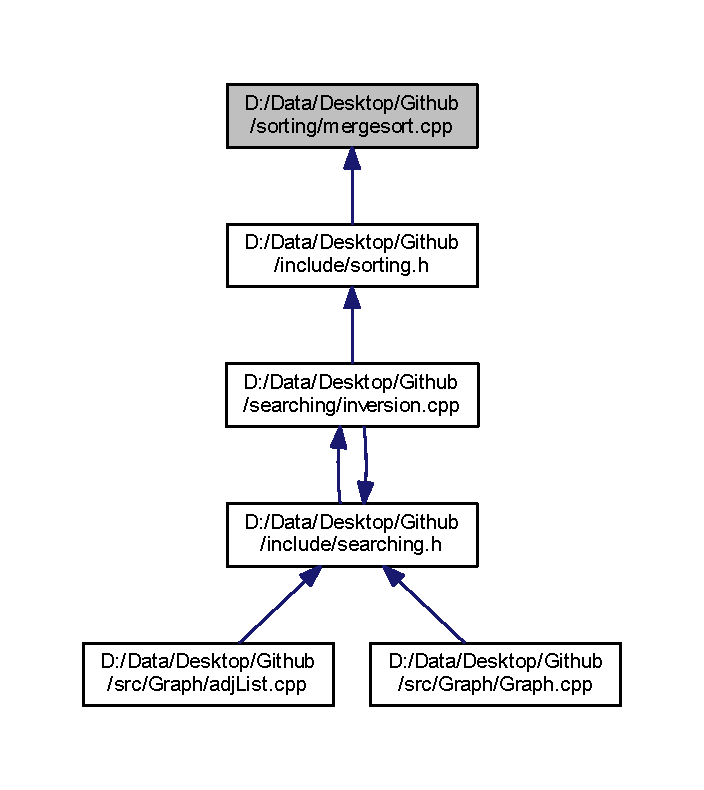
\includegraphics[width=338pt]{mergesort_8cpp__dep__incl}
\end{center}
\end{figure}
\subsection*{Namespaces}
\begin{DoxyCompactItemize}
\item 
 \hyperlink{namespace_alg_lib}{Alg\+Lib}
\end{DoxyCompactItemize}
\subsection*{Functions}
\begin{DoxyCompactItemize}
\item 
{\footnotesize template$<$typename T $>$ }\\T \hyperlink{namespace_alg_lib_a964728cae397746308b2d688e6f85d01}{Alg\+Lib\+::\+M\+E\+R\+GE} (T \&left, T \&right)
\item 
{\footnotesize template$<$typename T $>$ }\\void \hyperlink{namespace_alg_lib_a50103bb855668c829f3d0def288521a8}{Alg\+Lib\+::merge\+Sort} (T \&arr)
\begin{DoxyCompactList}\small\item\em Sort the elements in container arr with merge sort algorithm. \end{DoxyCompactList}\end{DoxyCompactItemize}

\hypertarget{_fraction_8cpp}{}\section{D\+:/\+Data/\+Desktop/\+Github/src/\+Fraction/\+Fraction.cpp File Reference}
\label{_fraction_8cpp}\index{D\+:/\+Data/\+Desktop/\+Github/src/\+Fraction/\+Fraction.\+cpp@{D\+:/\+Data/\+Desktop/\+Github/src/\+Fraction/\+Fraction.\+cpp}}
{\ttfamily \#include \char`\"{}Fraction.\+h\char`\"{}}\\*
{\ttfamily \#include $<$sstream$>$}\\*
Include dependency graph for Fraction.\+cpp\+:\nopagebreak
\begin{figure}[H]
\begin{center}
\leavevmode
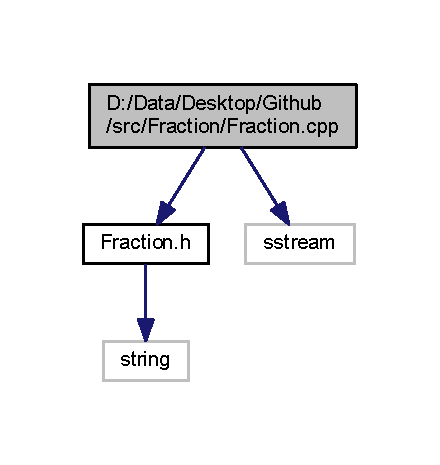
\includegraphics[width=211pt]{_fraction_8cpp__incl}
\end{center}
\end{figure}
\subsection*{Namespaces}
\begin{DoxyCompactItemize}
\item 
 \hyperlink{namespace_alg_lib}{Alg\+Lib}
\end{DoxyCompactItemize}
\subsection*{Functions}
\begin{DoxyCompactItemize}
\item 
Fraction \hyperlink{namespace_alg_lib_ade570114b2ba76f3c9742dd9ca92387c}{Alg\+Lib\+::operator+} (const Fraction \&f1, const Fraction \&f2)
\item 
Fraction \hyperlink{namespace_alg_lib_a8d6284ffd8dfa09154f65a0957ac6801}{Alg\+Lib\+::operator-\/} (const Fraction \&f1, const Fraction \&f2)
\item 
Fraction \hyperlink{namespace_alg_lib_aabcf6f54d813c4b6d701163009d268d9}{Alg\+Lib\+::operator$\ast$} (const Fraction \&f1, const Fraction \&f2)
\item 
Fraction \hyperlink{namespace_alg_lib_ab98deb23af06c328aede79f2fe4d2563}{Alg\+Lib\+::operator/} (const Fraction \&f1, const Fraction \&f2)
\end{DoxyCompactItemize}

\hypertarget{adj_list_8cpp}{}\section{D\+:/\+Data/\+Desktop/\+Github/src/\+Graph/adj\+List.cpp File Reference}
\label{adj_list_8cpp}\index{D\+:/\+Data/\+Desktop/\+Github/src/\+Graph/adj\+List.\+cpp@{D\+:/\+Data/\+Desktop/\+Github/src/\+Graph/adj\+List.\+cpp}}
{\ttfamily \#include \char`\"{}adj\+List.\+h\char`\"{}}\\*
{\ttfamily \#include \char`\"{}graph\+D\+B.\+h\char`\"{}}\\*
{\ttfamily \#include $<$vector$>$}\\*
{\ttfamily \#include $<$utility$>$}\\*
{\ttfamily \#include $<$tuple$>$}\\*
{\ttfamily \#include $<$stdexcept$>$}\\*
{\ttfamily \#include \char`\"{}searching.\+h\char`\"{}}\\*
Include dependency graph for adj\+List.\+cpp\+:\nopagebreak
\begin{figure}[H]
\begin{center}
\leavevmode
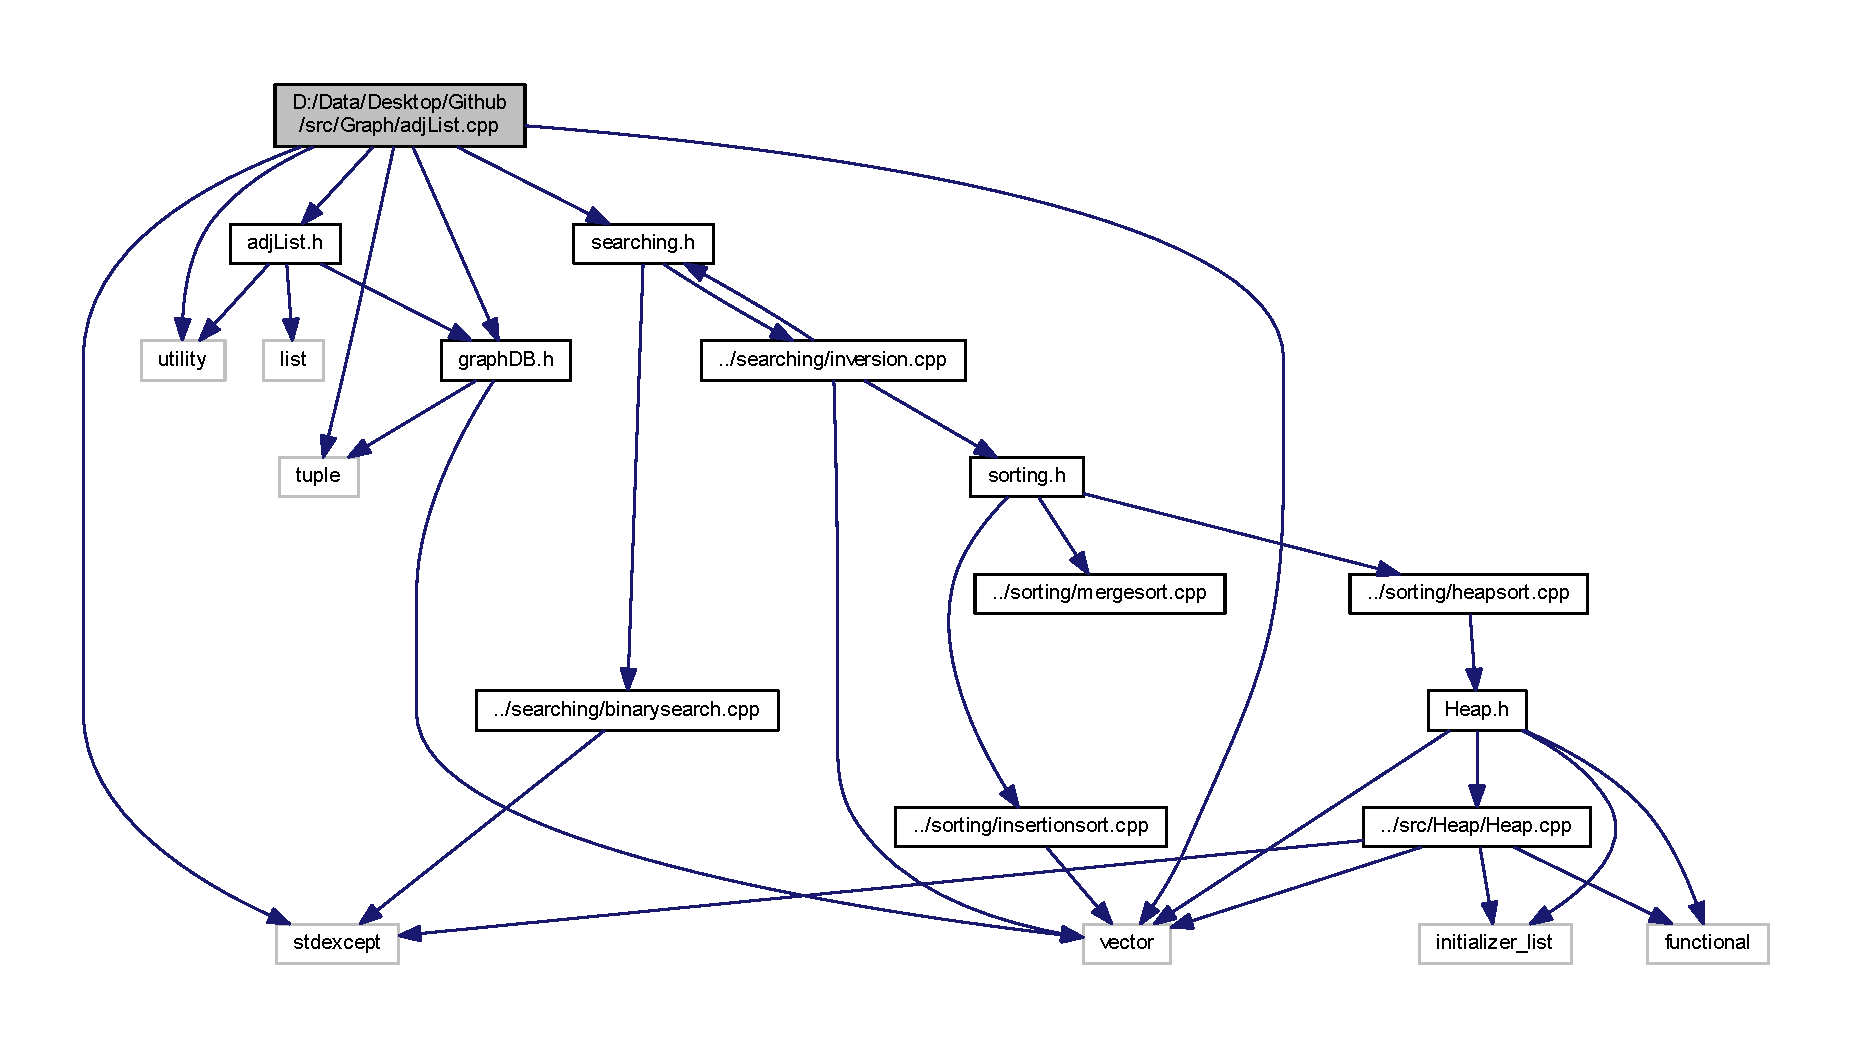
\includegraphics[width=350pt]{adj_list_8cpp__incl}
\end{center}
\end{figure}
\subsection*{Namespaces}
\begin{DoxyCompactItemize}
\item 
 \hyperlink{namespace_alg_lib}{Alg\+Lib}
\end{DoxyCompactItemize}

\hypertarget{adj_matrix_8cpp}{}\section{D\+:/\+Data/\+Desktop/\+Github/src/\+Graph/adj\+Matrix.cpp File Reference}
\label{adj_matrix_8cpp}\index{D\+:/\+Data/\+Desktop/\+Github/src/\+Graph/adj\+Matrix.\+cpp@{D\+:/\+Data/\+Desktop/\+Github/src/\+Graph/adj\+Matrix.\+cpp}}
{\ttfamily \#include \char`\"{}adj\+Matrix.\+h\char`\"{}}\\*
{\ttfamily \#include \char`\"{}Matrix.\+h\char`\"{}}\\*
{\ttfamily \#include \char`\"{}graph\+D\+B.\+h\char`\"{}}\\*
{\ttfamily \#include $<$vector$>$}\\*
{\ttfamily \#include $<$array$>$}\\*
Include dependency graph for adj\+Matrix.\+cpp\+:\nopagebreak
\begin{figure}[H]
\begin{center}
\leavevmode
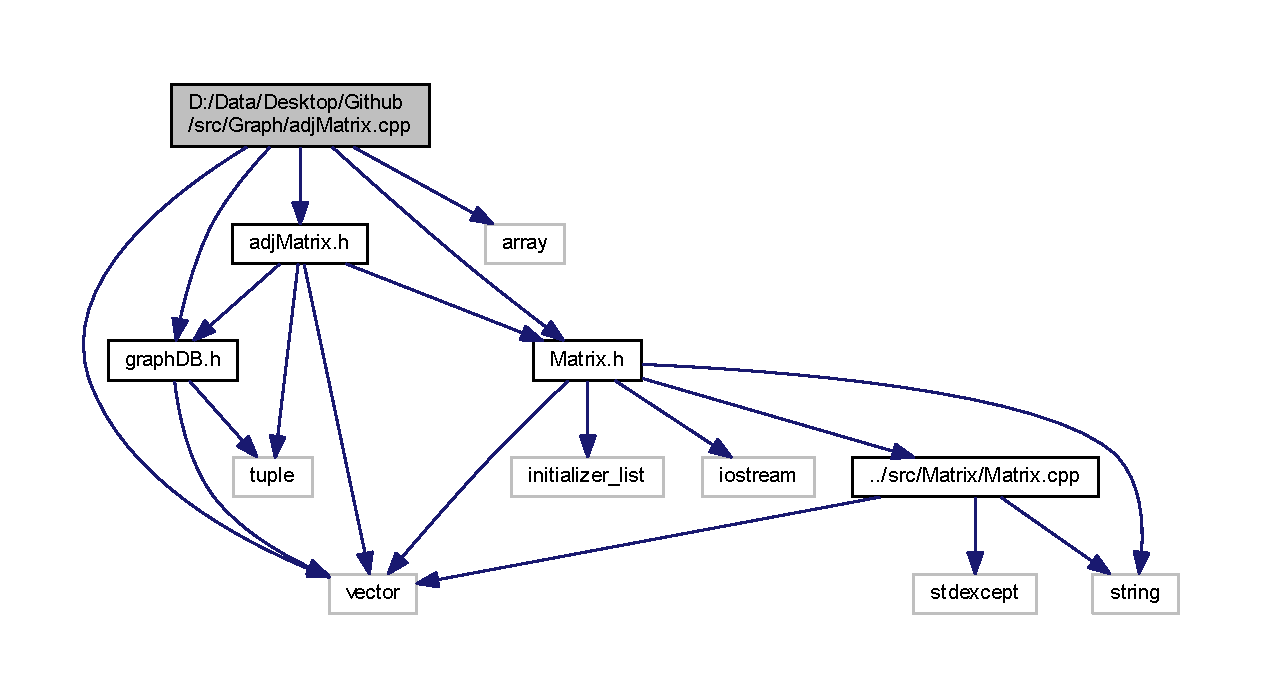
\includegraphics[width=350pt]{adj_matrix_8cpp__incl}
\end{center}
\end{figure}
\subsection*{Namespaces}
\begin{DoxyCompactItemize}
\item 
 \hyperlink{namespace_alg_lib}{Alg\+Lib}
\end{DoxyCompactItemize}

\hypertarget{_graph_8cpp}{}\section{D\+:/\+Data/\+Desktop/\+Github/src/\+Graph/\+Graph.cpp File Reference}
\label{_graph_8cpp}\index{D\+:/\+Data/\+Desktop/\+Github/src/\+Graph/\+Graph.\+cpp@{D\+:/\+Data/\+Desktop/\+Github/src/\+Graph/\+Graph.\+cpp}}
{\ttfamily \#include \char`\"{}Graph.\+h\char`\"{}}\\*
{\ttfamily \#include \char`\"{}graph\+D\+B.\+h\char`\"{}}\\*
{\ttfamily \#include \char`\"{}adj\+Matrix.\+h\char`\"{}}\\*
{\ttfamily \#include \char`\"{}adj\+List.\+h\char`\"{}}\\*
{\ttfamily \#include \char`\"{}Matrix.\+h\char`\"{}}\\*
{\ttfamily \#include \char`\"{}searching.\+h\char`\"{}}\\*
{\ttfamily \#include $<$tuple$>$}\\*
{\ttfamily \#include $<$utility$>$}\\*
Include dependency graph for Graph.\+cpp\+:\nopagebreak
\begin{figure}[H]
\begin{center}
\leavevmode
\includegraphics[width=350pt]{_graph_8cpp__incl}
\end{center}
\end{figure}
\subsection*{Namespaces}
\begin{DoxyCompactItemize}
\item 
 \hyperlink{namespace_alg_lib}{Alg\+Lib}
\end{DoxyCompactItemize}

\hypertarget{graph_d_b_8cpp}{}\section{D\+:/\+Data/\+Desktop/\+Github/src/\+Graph/graph\+DB.cpp File Reference}
\label{graph_d_b_8cpp}\index{D\+:/\+Data/\+Desktop/\+Github/src/\+Graph/graph\+D\+B.\+cpp@{D\+:/\+Data/\+Desktop/\+Github/src/\+Graph/graph\+D\+B.\+cpp}}
{\ttfamily \#include \char`\"{}graph\+D\+B.\+h\char`\"{}}\\*
{\ttfamily \#include $<$stdexcept$>$}\\*
Include dependency graph for graph\+D\+B.\+cpp\+:\nopagebreak
\begin{figure}[H]
\begin{center}
\leavevmode
\includegraphics[width=239pt]{graph_d_b_8cpp__incl}
\end{center}
\end{figure}
\subsection*{Namespaces}
\begin{DoxyCompactItemize}
\item 
 \hyperlink{namespace_alg_lib}{Alg\+Lib}
\end{DoxyCompactItemize}

\hypertarget{_heap_8cpp}{}\section{D\+:/\+Data/\+Desktop/\+Github/src/\+Heap/\+Heap.cpp File Reference}
\label{_heap_8cpp}\index{D\+:/\+Data/\+Desktop/\+Github/src/\+Heap/\+Heap.\+cpp@{D\+:/\+Data/\+Desktop/\+Github/src/\+Heap/\+Heap.\+cpp}}
{\ttfamily \#include $<$vector$>$}\\*
{\ttfamily \#include $<$initializer\+\_\+list$>$}\\*
{\ttfamily \#include $<$functional$>$}\\*
{\ttfamily \#include $<$stdexcept$>$}\\*
Include dependency graph for Heap.\+cpp\+:\nopagebreak
\begin{figure}[H]
\begin{center}
\leavevmode
\includegraphics[width=350pt]{_heap_8cpp__incl}
\end{center}
\end{figure}
This graph shows which files directly or indirectly include this file\+:\nopagebreak
\begin{figure}[H]
\begin{center}
\leavevmode
\includegraphics[width=338pt]{_heap_8cpp__dep__incl}
\end{center}
\end{figure}
\subsection*{Namespaces}
\begin{DoxyCompactItemize}
\item 
 \hyperlink{namespace_alg_lib}{Alg\+Lib}
\end{DoxyCompactItemize}

\hypertarget{_matrix_8cpp}{}\section{D\+:/\+Data/\+Desktop/\+Github/src/\+Matrix/\+Matrix.cpp File Reference}
\label{_matrix_8cpp}\index{D\+:/\+Data/\+Desktop/\+Github/src/\+Matrix/\+Matrix.\+cpp@{D\+:/\+Data/\+Desktop/\+Github/src/\+Matrix/\+Matrix.\+cpp}}
{\ttfamily \#include $<$vector$>$}\\*
{\ttfamily \#include $<$string$>$}\\*
{\ttfamily \#include $<$stdexcept$>$}\\*
Include dependency graph for Matrix.\+cpp\+:\nopagebreak
\begin{figure}[H]
\begin{center}
\leavevmode
\includegraphics[width=259pt]{_matrix_8cpp__incl}
\end{center}
\end{figure}
This graph shows which files directly or indirectly include this file\+:\nopagebreak
\begin{figure}[H]
\begin{center}
\leavevmode
\includegraphics[width=350pt]{_matrix_8cpp__dep__incl}
\end{center}
\end{figure}
\subsection*{Namespaces}
\begin{DoxyCompactItemize}
\item 
 \hyperlink{namespace_alg_lib}{Alg\+Lib}
\end{DoxyCompactItemize}

\hypertarget{_permutation_8cpp}{}\section{D\+:/\+Data/\+Desktop/\+Github/src/\+Permutation/\+Permutation.cpp File Reference}
\label{_permutation_8cpp}\index{D\+:/\+Data/\+Desktop/\+Github/src/\+Permutation/\+Permutation.\+cpp@{D\+:/\+Data/\+Desktop/\+Github/src/\+Permutation/\+Permutation.\+cpp}}
{\ttfamily \#include $<$initializer\+\_\+list$>$}\\*
{\ttfamily \#include $<$vector$>$}\\*
{\ttfamily \#include $<$exception$>$}\\*
{\ttfamily \#include $<$algorithm$>$}\\*
{\ttfamily \#include $<$utility$>$}\\*
{\ttfamily \#include \char`\"{}..\textbackslash{}..\textbackslash{}include\textbackslash{}\+Permutation.\+h\char`\"{}}\\*
Include dependency graph for Permutation.\+cpp\+:\nopagebreak
\begin{figure}[H]
\begin{center}
\leavevmode
\includegraphics[width=350pt]{_permutation_8cpp__incl}
\end{center}
\end{figure}
This graph shows which files directly or indirectly include this file\+:\nopagebreak
\begin{figure}[H]
\begin{center}
\leavevmode
\includegraphics[width=243pt]{_permutation_8cpp__dep__incl}
\end{center}
\end{figure}

\hypertarget{_int_polynomial_8cpp}{}\section{D\+:/\+Data/\+Desktop/\+Github/src/\+Polynomial/\+Int\+Polynomial.cpp File Reference}
\label{_int_polynomial_8cpp}\index{D\+:/\+Data/\+Desktop/\+Github/src/\+Polynomial/\+Int\+Polynomial.\+cpp@{D\+:/\+Data/\+Desktop/\+Github/src/\+Polynomial/\+Int\+Polynomial.\+cpp}}
{\ttfamily \#include $<$vector$>$}\\*
{\ttfamily \#include $<$stdexcept$>$}\\*
{\ttfamily \#include \char`\"{}Polynomial.\+h\char`\"{}}\\*
Include dependency graph for Int\+Polynomial.\+cpp\+:\nopagebreak
\begin{figure}[H]
\begin{center}
\leavevmode
\includegraphics[width=350pt]{_int_polynomial_8cpp__incl}
\end{center}
\end{figure}

\hypertarget{_polynomial_8cpp}{}\section{D\+:/\+Data/\+Desktop/\+Github/src/\+Polynomial/\+Polynomial.cpp File Reference}
\label{_polynomial_8cpp}\index{D\+:/\+Data/\+Desktop/\+Github/src/\+Polynomial/\+Polynomial.\+cpp@{D\+:/\+Data/\+Desktop/\+Github/src/\+Polynomial/\+Polynomial.\+cpp}}
{\ttfamily \#include $<$initializer\+\_\+list$>$}\\*
Include dependency graph for Polynomial.\+cpp\+:\nopagebreak
\begin{figure}[H]
\begin{center}
\leavevmode
\includegraphics[width=234pt]{_polynomial_8cpp__incl}
\end{center}
\end{figure}
This graph shows which files directly or indirectly include this file\+:\nopagebreak
\begin{figure}[H]
\begin{center}
\leavevmode
\includegraphics[width=244pt]{_polynomial_8cpp__dep__incl}
\end{center}
\end{figure}

%--- End generated contents ---

% Index
\backmatter
\newpage
\phantomsection
\clearemptydoublepage
\addcontentsline{toc}{chapter}{Index}
\printindex

\end{document}
